\section*{Développement démonstratif du noyau commun}
\addcontentsline{toc}{section}{Développement démonstratif du noyau commun}

Les constructions suivantes développent les règles d'émission, le calendrier avec mémoire, les suites compatibles, la complétion cubique, les lecteurs régionaux et la réversibilité du registre dodécaphasique. Leurs définitions et démonstrations précèdent les applications arithmétiques et spectrales qui les utilisent. Les fragments provenant de l'article I conservent leurs énoncés, preuves et localisateurs ; le manifeste des sources identifie les composants, intervalles et empreintes correspondants.

Les mentions d'alpha et du corridor exceptionnel précisent la provenance des objets. Les identifications ultérieures avec des codes et des réseaux n'interviennent pas dans les preuves spectrales de ce manuscrit. Les renvois à l'article I documentent cette provenance, tandis que les arguments nécessaires sont présentés ici intégralement. Les recensements finis et les reconstructions sont interprétés avec les règles, domaines et coordonnées de départ de chaque énoncé ; leur incorporation ne modifie pas la portée de la positivité globale déclarée dans le résumé.

% BEGIN NUCLEO_ADITIVO_20260921_CENSO
\clearpage
\section{Noyau topologique de phase et génération du catalogue de germes}
\label{act21:tpk:capitulo}

Les deux évaluations de l'APP acquièrent une efficacité générative lorsque l'on précise
quelle évaluation agit, en quelle position elle s'effectue, comment cette position se déplace
et quelle information chaque transition conserve. Le \emph{Topological Phase Kernel},
abrégé en TPK et dénommé en espagnol \emph{núcleo topológico de fase}, réunit
ces opérations dans une dynamique sur des états enrichis. Sa définition
comprend la sélection, le transport, la mise à jour arithmétique et la conservation du
registre. La construction finie développée dans ce chapitre fournit
les germes sur lesquels agiront les relèvements régionaux et le prolongement
coinductif.

Le résultat principal de cette étape est un catalogue généré et classé :
les conditions initiales des deux curseurs produisent des émissions entières ;
leur lecture ternaire détermine des mots orientés ; l'action diédrale organise
ces mots en orbites. Chaque étape conserve ses préimages et les relations
qui permettent de revenir à la description précédente. La chaîne de cardinaux
\[
 104\,976\longrightarrow468\longrightarrow243\subset729,
 \qquad 243\longrightarrow43,
\]
désigne sous une forme abrégée des objets différents. Chaque objet est ensuite construit et chaque dénombrement
est justifié, avant que l'un d'eux soit utilisé comme donnée de
la sélection régionale.

\subsection{Sélection de phase, transport et état enrichi}
\label{act21:tpk:operaciones}

\subsubsection{Sélecteur tritique de phase opérationnelle}

La phase nonadique prend ses valeurs en \(D_9=\{1,\ldots,9\}\). Le sélecteur  
tritique est la fonction
\begin{equation}
 M_{\mathrm{ph}}:D_9\longrightarrow\{-1,0,+1\},\qquad
 M_{\mathrm{ph}}(g)=
 \begin{cases}
 +1,&g\in\{1,4,7\},\\
 -1,&g\in\{2,5,8\},\\
 0,&g\in\{3,6,9\}.
 \end{cases}
 \label{act21:tpk:selector}
\end{equation}
Dans la réalisation émettrice, la valeur \(+1\) active l'évaluation additive,
\(-1\) active l'évaluation multiplicative et \(0\) enregistre l'événement
neutre. L'orientation cardinale du curseur est une autre coordonnée de l'état.
Cette séparation permet de fixer simultanément quelle opération est lue et dans quelle
direction est transporté son point d'évaluation.

Pour les transitions numérotées par \(t\geq1\), la phase précédant la lecture est
\begin{equation}
 g_t=1+[(t-1)]_9,\qquad \epsilon_t=M_{\mathrm{ph}}(g_t),
 \label{act21:tpk:fase}
\end{equation}
où \([n]_b\) désigne le représentant de \(n\) modulo \(b\) dans
\(\{0,\ldots,b-1\}\). Une fenêtre de neuf transitions contient la suite
\((+1,-1,0,+1,-1,0,+1,-1,0)\).

\subsubsection{Curseurs orientés et transport cardinal}

Des indices \(I_9=\{0,\ldots,8\}\) sont utilisés pour les positions et des étiquettes positives \((a,b)=(i+1,j+1)\) pour les évaluations APP. Un curseur fini est
\[
 c=(i,j;d)\in\mathcal S:=I_9^2\times\mathcal D,
 \qquad \mathcal D=\{N,E,S,O\}.
\]
Les quatre directions agissent par
\[
 v_N=(-1,0),\quad v_E=(0,1),\quad
 v_S=(1,0),\quad v_O=(0,-1).
\]
L'application cardinale correspondant à \(d\) est
\[
 T_d(i,j)=\bigl([i+(v_d)_1]_9,[j+(v_d)_2]_9\bigr).
\]
Ainsi, \(M_{\mathrm{ph}}\) et \(T_d\) ont des domaines, des codomaines et des actions différents. L'activation tritique sélectionne l'un des deux curseurs ; le transport cardinal modifie sa position dans la direction que ce curseur conserve déjà.

Le relèvement entier du curseur est
\(\widetilde c=(x,y;d)\in\mathbb Z^2\times\mathcal D\), avec position finie
\(([x]_9,[y]_9)\). Ses nombres de tours sont récupérés en
\begin{equation}
 x=9\lfloor x/9\rfloor+[x]_9,\qquad
 y=9\lfloor y/9\rfloor+[y]_9.
 \label{act21:tpk:vueltas}
\end{equation}
Ces deux divisions concernent le transport spatial. La division d'une
évaluation additive ou multiplicative constitue un registre arithmétique
distinct, qui sera conservé conjointement avec elles.

\subsubsection{Composition de la transition}

L'état de la réalisation finie comprend les deux curseurs relevés,
leurs directions, la phase, les accumulateurs de la fenêtre active, la liste
ordonnée des blocs déjà émis et le registre des transitions. Chaque registre
local contient les positions antérieures, les évaluations entières des deux
feuillets, leurs restes et quotients, le régime actif et les orientations.
Les champs de préfixe et de frontière qui apparaîtront dans un prolongement seront
incorporés au même état avec leurs règles de compatibilité.

La transition s'ordonne comme
\begin{equation}
 \mathcal U_t=\mathsf{Mem}_t\circ\mathsf{Tra}_t\circ\mathsf{Sel}_t.
 \label{act21:tpk:composicion}
\end{equation}
La sélection détermine le régime et conserve l'échantillon antérieur à tout déplacement. Le transport applique le mouvement actif et l'inversion cardinale prescrite par le calendrier. L'actualisation incorpore cet échantillon aux accumulateurs et au registre ; à la fin d'une fenêtre, elle émet son bloc. La composition utilise donc un échantillon antérieur au transport bien que son archivage définitif s'effectue à la fin de la transition.

\subsection{Conditions initiales et énumération réversible}
\label{act21:tpk:semillas}

Les feuillets additif et multiplicatif disposent de curseurs indépendants. Le
domaine des conditions initiales est le produit ordonné
\[
 \Omega_{\mathrm{seed}}=\mathcal S_+\times\mathcal S_\times,
 \qquad |\mathcal S|=9^2\cdot4=324.
\]
Par conséquent,
\begin{equation}
 |\Omega_{\mathrm{seed}}|=324^2=104\,976.
 \label{act21:tpk:censo-inicial}
\end{equation}
Le nombre \(81\) compte des positions ; \(324\) compte des positions orientées d'un curseur ; \(104\,976\) compte des paires ordonnées de curseurs. Le choix d'une position en APP conserve uniquement une partie d'une condition initiale de l'émetteur.

On fixe la numérotation
\[
 \operatorname{ind}(N)=0,\quad\operatorname{ind}(E)=1,\quad
 \operatorname{ind}(S)=2,\quad\operatorname{ind}(O)=3,
\]
et l'on définit
\begin{equation}
 \nu(i,j;d)=4(9i+j)+\operatorname{ind}(d).
 \label{act21:tpk:indice-semilla}
\end{equation}

\begin{proposition}[Énumération exacte des conditions initiales]
\label{act21:tpk:enumeracion}
L'application \(\nu\) est une bijection de \(\mathcal S\) sur
\(\{0,\ldots,323\}\). Le couple d'indices se code de manière réversible
par \(324\nu_++\nu_\times\in\{0,\ldots,104\,975\}\).
\end{proposition}
\begin{proof}
La division par quatre restaure
\[
 \operatorname{ind}(d)=[\nu]_4,\qquad
 j=[\lfloor\nu/4\rfloor]_9,\qquad i=\lfloor\nu/36\rfloor.
\]
Les bornes du domaine garantissent que ces trois quantités appartiennent à
leurs ensembles d'indices et reconstruisent \(\nu\) au moyen de
\eqref{act21:tpk:indice-semilla}. Pour le couple, la division euclidienne par
\(324\) restitue le quotient \(\nu_+\) et le reste \(\nu_\times\).
\end{proof}

L'énumération parcourt le domaine complet avant tout regroupement
régional. Les indices servent à localiser les préimages d'une
émission, en conservant explicitement la condition qui a produit chaque trajectoire.

\subsection{Évaluation des feuillets et registre arithmétique}
\label{act21:tpk:lecturas}

En une position positive \((a,b)\), les évaluations entières sont
\(A_+(a,b)=a+b\) et \(A_\times(a,b)=ab\). Pour \(n>0\), on conserve
\begin{equation}
 \rho_9(n)=1+[n-1]_9,\qquad
 q_9(n)=\lfloor(n-1)/9\rfloor,\qquad
 n=\rho_9(n)+9q_9(n).
 \label{act21:tpk:division-evaluacion}
\end{equation}
L'activation additive incorpore \(\rho_9(A_+)\) à l'accumulateur correspondant. L'activation multiplicative utilise un observable du résidu \(\rho_9(A_\times)\), défini ci-dessous.

\subsubsection{Exposant discret dans les unités modulo neuf}

Les puissances de \(2\) modulo \(9\) parcourent
\[
 2^0,2^1,\ldots,2^5\equiv1,2,4,8,7,5\pmod9,
 \qquad 2^6\equiv1\pmod9.
\]
Le logarithme discret dans ce groupe de six unités se représente par
\begin{equation}
 \ell_9(1)=0,\quad\ell_9(2)=1,\quad\ell_9(4)=2,
 \quad\ell_9(8)=3,\quad\ell_9(7)=4,\quad\ell_9(5)=5.
 \label{act21:tpk:logaritmo}
\end{equation}
La loi émettrice étend l'observable par le biais de \(\ell_9(3)=\ell_9(6)=\ell_9(9)=0\). Pour conserver son origine, l'échantillon enregistré inclut le résidu original et l'indicateur d'appartenance au groupe d'unités. Ainsi, une valeur observée nulle peut provenir de l'unité \(1\) ou de l'un des trois résidus non inversibles, et son origine demeure récupérable.

\subsubsection{Ordre de lecture et mouvement}

Les évaluations s'effectuent aux positions antérieures à la transition.
Si \(\epsilon_t=+1\), on accumule la lecture additive et on déplace son curseur.
Si \(\epsilon_t=-1\), on accumule l'exposant discret multiplicatif et on
déplace le second curseur. Si \(\epsilon_t=0\), on incrémente le compteur
neutre et on conserve les deux positions.

À la fin des étapes \(27\) et \(54\), les deux directions sont remplacées
par leurs opposées. Les fenêtres s'enchaînent en conservant leurs positions et
orientations. Au début de chaque fenêtre, seuls ses trois accumulateurs locaux sont remis à zéro ; le registre précédent reste disponible.

\begin{proposition}[Inversion du transport relevé]
\label{act21:tpk:inversion}
Soient \(a,b\in\{0,1\}\) les indicateurs d'activation et d'inversion d'un
curseur. Si \(\operatorname{opp}\) échange \(N\leftrightarrow S\) et
\(E\leftrightarrow O\), la transformation
\[
 F_{a,b}(z,d)=\bigl(z+a v_d,\operatorname{opp}^{\,b}(d)\bigr)
\]
admet pour inverse
\[
 F_{a,b}^{-1}(z',d')=
 \bigl(z'-a v_{\operatorname{opp}^{\,b}(d')},
       \operatorname{opp}^{\,b}(d')\bigr).
\]
La réduction spatiale modulo neuf entrelace cette transformation avec le
transport fini.
\end{proposition}
\begin{proof}
Appliquer deux fois l'opposition restaure la direction initiale. Une fois
cette direction récupérée, la soustraction de \(a v_d\) annule le déplacement.
Pour la projection spatiale, il suffit de l'égalité
\([z+a v_d]_9=[[z]_9+a v_d]_9\), composante par composante. L'inversion de
direction conserve cette égalité.
\end{proof}

La phase détermine les indicateurs utilisés par l'inverse. Le registre
spatial et l'arithmétique peuvent ainsi être conservés conjointement, même en
traversant le bord du représentant \(I_9^2\).

\subsection{Six fenêtres et émission décimale par blocs}
\label{act21:tpk:emision}

\subsubsection{Accumulation dans une fenêtre nonadique}

La fenêtre \(m\), avec \(1\leq m\leq6\), comprend les étapes
\(9m-8,\ldots,9m\). Soient \(S_m\) la somme de ses résidus positifs
additifs actifs, \(E_m\) la somme de ses exposants discrets actifs et
\(Z_m\) son nombre d'événements neutres.

\begin{lemma}[Multiplicités d'activation]
\label{act21:tpk:tres-eventos}
Chaque fenêtre contient trois activations additives, trois multiplicatives et
trois neutres. En particulier, \(Z_m=3\).
\end{lemma}
\begin{proof}
Les phases d'une fenêtre parcourent exactement \(1,\ldots,9\). Chacun
des trois ensembles de \eqref{act21:tpk:selector} a pour cardinal trois.
\end{proof}

Les six fenêtres forment \(54\) transitions et produisent six blocs.  
Cette longueur appartient à l'émetteur initial défini ici. La continuation  
en profondeur agit ensuite sur les mots et leurs registres compatibles.

\subsubsection{Règle de codification décimale}

La loi émettrice spécifie les chiffres
\begin{align}
 d_{m,1}&=[S_m]_{10},\notag\\
 d_{m,2}&=[S_m+E_m]_{10},\notag\\
 d_{m,3}&=[3S_m+5E_m+7Z_m]_{10},\notag\\
 U_m&=100d_{m,1}+10d_{m,2}+d_{m,3}.
 \label{act21:tpk:bloque-decimal}
\end{align}
Les poids \(100,10,1\) sont les positions des centaines, des dizaines et des unités.
L'indice \(10\) indique le reste décimal, et chaque bloc satisfait
\(0\leq U_m\leq999\). Le mot émis est la suite ordonnée
\(\mathbf U=(U_1,\ldots,U_6)\), de largeur fixe de trois chiffres par bloc.

Les coefficients \(3,5,7\) constituent les poids explicites de cette loi
émettrice. Une fois la règle fixée, chaque chiffre se calcule à partir des
accumulateurs, et les résultats de ce chapitre se déduisent de cette règle.
Le nombre \(1\) qui apparaît sous sa forme réduite a une origine
additionnelle concrète : \(7Z_m=21\equiv1\pmod{10}\).

Si \(s_m=[S_m]_{10}\) et \(e_m=[E_m]_{10}\), on obtient
\begin{equation}
 G(s_m,e_m)=100s_m+10[s_m+e_m]_{10}
                   +[3s_m+5e_m+1]_{10}=U_m.
 \label{act21:tpk:acoplamiento-firmas}
\end{equation}
La lettre \(e_m\) désigne ici une composante de la signature d'exposants discrets. Sa définition appartient à l'émetteur fini.

\begin{proposition}[Récupération des deux signatures]
\label{act21:tpk:recuperacion-firmas}
L'application \(G:\{0,\ldots,9\}^2\to\{0,\ldots,999\}\) est injective.
Pour un bloc \(U=100a+10b+c\) de son image, l'inverse est
\[
 s=a,\qquad e=[b-a]_{10},\qquad
 c=[3s+5e+1]_{10}.
\]
En conséquence, le mot \(\mathbf U\) détermine les deux signatures de six composantes \(\mathbf s\) et \(\mathbf e\).
\end{proposition}
\begin{proof}
Les deux derniers termes de \eqref{act21:tpk:acoplamiento-firmas} appartiennent à
\(\{0,\ldots,99\}\), de sorte que la centaine récupère \(s\). La dizaine
est \([s+e]_{10}\) ; en soustrayant \(s\) et en réduisant modulo dix, on récupère
\(e\). L'unité vérifie la troisième congruence. La reconstruction s'applique
indépendamment aux six positions du mot.
\end{proof}

Les totaux entiers \(S_m,E_m\) se retrouvent à partir des lectures enregistrées ;
les centaines et les dizaines retrouvent leurs restes. Par exemple, un total
\(S_m=15\) produit \(s_m=5\). Cette différence identifie exactement
quelle information chaque niveau de codage conserve.

\subsubsection{Codification positionnelle du mot de six blocs}

Les six blocs admettent une codification entière à largeur fixe,
\begin{equation}
 \mathscr N(\mathbf U)=\sum_{m=1}^{6}U_m1000^{6-m},
 \qquad0\leq\mathscr N(\mathbf U)<1000^6.
 \label{act21:tpk:entero-base1000}
\end{equation}
Le premier bloc occupe la position de plus haut poids et le sixième, celle des unités de base mille. Un bloc \(058\) occupe une position complète avec une valeur entière \(58\) ; sa largeur de trois chiffres fait partie de la présentation décimale de cette position.

\begin{proposition}[Récupération positionnelle des émissions]
\label{act21:tpk:inversa-base1000}
La codification \eqref{act21:tpk:entero-base1000} détermine le mot complet
par le biais de
\[
 U_m=\left[\left\lfloor
 \frac{\mathscr N(\mathbf U)}{1000^{6-m}}\right\rfloor\right]_{1000},
 \qquad1\leq m\leq6.
\]
\end{proposition}
\begin{proof}
En divisant par \(1000^{6-m}\), les blocs précédents produisent des multiples entiers de \(1000\), le bloc \(m\) produit \(U_m\), et la contribution des suivants appartient à \([0,1)\). La partie entière élimine cette dernière contribution et le résidu modulo \(1000\) élimine les premières.
\end{proof}

Cette codification conserve les six émissions. Son domaine possède des positions ordonnées de base mille, tandis que le domaine APP possède des positions spatiales modulo neuf. La composition maintient les deux indices : \(m\) identifie une fenêtre d'émission et \((i,j)\) identifie la cellule visitée lors d'une transition de cette fenêtre.

\subsection{Calcul complet d'une émission qui commence par 501}
\label{act21:tpk:ejemplo501}

On fixe les conditions initiales
\[
 c_{+,0}=(0,4;N),\qquad c_{\times,0}=(2,3;N),
 \qquad \nu_+=16,\quad\nu_\times=84.
\]
Les positions positives initiales sont \((1,5)\) et \((3,4)\). L'indice
chronologique précédent est \(t=0\), la première phase lue est \(g_1=1\) et le
registre est vide. Ces coordonnées sont les entrées
du calcul ; les blocs s'obtiennent en exécutant la récurrence.

\begin{table}[htbp]
\caption{Première fenêtre : lectures précédentes et accumulation active.}
\label{act21:tpk:tabla-501}
\small
\begin{tabular}{@{}rcccrrr@{}}
\toprule
\(t\)&\(\epsilon_t\)&position \(+\)&position \(\times\)&
\(\Delta S\)&\(\Delta E\)&\((S,E,Z)\)\\
\midrule
1&\(+1\)&\((1,5)\)&\((3,4)\)&6&0&\((6,0,0)\)\\
2&\(-1\)&\((9,5)\)&\((3,4)\)&0&0&\((6,0,0)\)\\
3&0&\((9,5)\)&\((2,4)\)&0&0&\((6,0,1)\)\\
4&\(+1\)&\((9,5)\)&\((2,4)\)&5&0&\((11,0,1)\)\\
5&\(-1\)&\((8,5)\)&\((2,4)\)&0&3&\((11,3,1)\)\\
6&0&\((8,5)\)&\((1,4)\)&0&0&\((11,3,2)\)\\
7&\(+1\)&\((8,5)\)&\((1,4)\)&4&0&\((15,3,2)\)\\
8&\(-1\)&\((7,5)\)&\((1,4)\)&0&2&\((15,5,2)\)\\
9&0&\((7,5)\)&\((9,4)\)&0&0&\((15,5,3)\)\\
\bottomrule
\end{tabular}
\notatabla{Les positions sont des étiquettes positives des cellules antérieures au mouvement. Les événements neutres augmentent uniquement \(Z\).}
\end{table}

Les trois évaluations additives actives sont
\[
 1+5=6,\qquad9+5=14=5+9,\qquad8+5=13=4+9,
\]
de telle sorte que \(S_1=6+5+4=15\). Les trois évaluations multiplicatives actives
sont \(3\cdot4=12\), \(2\cdot4=8\) et \(1\cdot4=4\). Leurs résidus
positifs sont \(3,8,4\), avec des observables \(0,3,2\) ; par conséquent,
\(E_1=5\). Enfin \(Z_1=3\). La règle décimale donne
\[
 d_{1,1}=[15]_{10}=5,\quad
 d_{1,2}=[15+5]_{10}=0,\quad
 d_{1,3}=[45+25+21]_{10}=1,
\]
et on obtient \(U_1=501\).

La seconde lecture additive précédente a pour quotient arithmétique \(1\),
tandis que son curseur relevé se trouve en \((-1,4;N)\), avec un nombre de tours
verticaux \(-1\). Ce sont deux données différentes du même registre. Toutes deux
interviennent dans la récupération intégrale de l'évaluation et de sa position.

\begin{table}[htbp]
\caption{Les six fenêtres de la condition initiale \((16,84)\).}
\label{act21:tpk:tabla-seis501}
\begin{tabular}{@{}rrrrrrrr@{}}
\toprule
\(m\)&pas&\(S_m\)&\(E_m\)&\(Z_m\)&\(s_m\)&\(U_m\)&\([-U_m]_3\)\\
\midrule
1&1--9&15&5&3&5&501&0\\
2&10--18&6&5&3&6&614&1\\
3&19--27&24&5&3&4&498&0\\
4&28--36&21&5&3&1&169&2\\
5&37--45&12&5&3&2&272&1\\
6&46--54&12&5&3&2&272&1\\
\bottomrule
\end{tabular}
\end{table}

Le mot résultant et ses signatures sont
\begin{align*}
 \mathbf U&=(501,614,498,169,272,272),\\
 \mathbf s&=(5,6,4,1,2,2),&
 \mathbf e&=(5,5,5,5,5,5).
\end{align*}
L'inversion cardinale après l'étape \(27\) modifie les parcours des
trois fenêtres finales. Le bloc répété \(272\) correspond à deux
fenêtres successives possédant leurs propres positions et leur propre registre chronologique.

Comme deuxième cas, la condition initiale minimale \((\nu_+,\nu_\times)=(0,0)\)
produit
\[
 \mathbf U=(252,109,252,903,850,850),\quad
 \mathbf s=(2,1,2,9,8,8),\quad
 \mathbf e=(3,9,3,1,7,7).
\]
Dans ce cas, les deux curseurs retournent à leur position et orientation initiales
après \(54\) transitions. La phase nonadique effectue six tours, le
compteur chronologique avance de \(54\) unités et le registre contient
\(54\) échantillons. La lecture positionnelle du retour et
l'histoire enregistrée décrivent des propriétés distinctes de l'exécution.

\subsection{Factorisation du recensement fini}
\label{act21:tpk:censo}

Les signatures \(f_+(\nu)=\mathbf s\) et \(f_\times(\nu)=\mathbf e\) se
calculent en exécutant le curseur correspondant pendant les six fenêtres.
L'indépendance des positions et des directions entre les deux curseurs donne
\begin{equation}
 T_{\mathrm{em}}(\nu_+,\nu_\times)
   =G^{(6)}\bigl(f_+(\nu_+),f_\times(\nu_\times)\bigr),
 \label{act21:tpk:factorizacion}
\end{equation}
où \(G^{(6)}\) applique \eqref{act21:tpk:acoplamiento-firmas} à chaque position.
La factorisation permet d'énumérer d'abord \(324+324\) trajectoires et
de combiner ensuite les signatures distinctes, en conservant la multiplicité de
leurs préimages.

\par\noindent\begin{minipage}{\linewidth}
\subsubsection{Images des deux signatures}

Les tableaux suivants comprennent toutes les signatures. Leur multiplicité est le
nombre de conditions initiales qui les produisent ; l'indice minimal localise
l'une de ces conditions. La préimage complète est définie par
\[
 f_\sigma^{-1}(a)=\{\nu\in\{0,\ldots,323\}:f_\sigma(\nu)=a\}.
\]
La récurrence des sections précédentes détermine chaque élément de cet
ensemble par un calcul entier fini.

\begin{table}[H]
\centering\fontsize{9.5}{11.4}\selectfont
\setlength{\abovecaptionskip}{8pt}\setlength{\belowcaptionskip}{6pt}
\renewcommand{\arraystretch}{1.12}
\caption{Les dix-huit signatures additives.}
\label{act21:tpk:firmas-aditivas}
\begin{tabular}{@{}lrr@{\qquad}lrr@{}}
\toprule
signature&multiplicité&\(\nu_{\min}\)&signature&multiplicité&\(\nu_{\min}\)\\
\midrule
\texttt{122564}&18&17&\texttt{564122}&18&16\\
\texttt{122898}&18&24&\texttt{645212}&18&4\\
\texttt{212645}&18&5&\texttt{654889}&18&33\\
\texttt{212988}&18&0&\texttt{889221}&18&13\\
\texttt{221456}&18&29&\texttt{889654}&18&32\\
\texttt{221889}&18&12&\texttt{898122}&18&25\\
\texttt{456221}&18&28&\texttt{898465}&18&20\\
\texttt{465898}&18&21&\texttt{988212}&18&1\\
\texttt{546988}&18&9&\texttt{988546}&18&8\\
\bottomrule
\end{tabular}

\par\vspace{12pt}

\caption{Les vingt-six signatures multiplicatives.}
\label{act21:tpk:firmas-multiplicativas}
\begin{tabular}{@{}lrr@{\qquad}lrr@{}}
\toprule
signature&multiplicité&\(\nu_{\min}\)&signature&multiplicité&\(\nu_{\min}\)\\
\midrule
\texttt{000000}&108&8&\texttt{555555}&24&84\\
\texttt{177393}&8&1&\texttt{555717}&8&14\\
\texttt{177555}&8&54&\texttt{555771}&8&18\\
\texttt{177771}&8&11&\texttt{555933}&8&24\\
\texttt{339555}&8&6&\texttt{717555}&8&12\\
\texttt{339771}&8&15&\texttt{717717}&8&21\\
\texttt{339933}&8&59&\texttt{717933}&8&19\\
\texttt{393177}&8&0&\texttt{771177}&8&9\\
\texttt{393393}&8&45&\texttt{771339}&8&13\\
\texttt{393555}&8&40&\texttt{771555}&8&16\\
\texttt{555177}&8&52&\texttt{933339}&8&57\\
\texttt{555339}&8&4&\texttt{933555}&8&26\\
\texttt{555393}&8&41&\texttt{933717}&8&17\\
\bottomrule
\end{tabular}
\end{table}
\end{minipage}\par


\begin{proposition}[Image et multiplicités de l'émetteur]
\label{act21:tpk:468}
L'image \(\mathcal U_6=\operatorname{im}T_{\mathrm{em}}\) contient
\(468\) mots distincts. Ses préimages se répartissent en \(432\)
fibres de cardinal \(144\), \(18\) de cardinal \(432\) et \(18\) de
cardinal \(1944\).
\end{proposition}
\begin{proof}
L'évaluation exhaustive de l'algorithme de la section ~\ref{act21:tpk:algoritmo} sur les indices \(0,\ldots,323\) donne les deux tableaux ci-dessus. La première partition a \(18\) classes de cardinal \(18\), et la seconde \(24\) classes de cardinal \(8\), une de cardinal \(24\) et une de cardinal \(108\). Les sommes \(18\cdot18=324\) et \(24\cdot8+24+108=324\) vérifient la masse totale des deux partitions. La proposition ~\ref{act21:tpk:recuperacion-firmas} rend injectif le couplage de ses images ; par conséquent, il y a \(18\cdot26=468\) émissions. Par \eqref{act21:tpk:factorizacion}, la préimage d'un couple de signatures est le produit de ses deux préimages. On obtient \(18\cdot24=432\) produits de cardinal \(18\cdot8=144\), \(18\) de cardinal \(18\cdot24=432\) et \(18\) de cardinal \(18\cdot108=1944\). Enfin,
\[
 432\cdot144+18\cdot432+18\cdot1944=104\,976.
\]
La partie énumérative est une vérification finie exacte de la récurrence ;
la factorisation explique pourquoi ce décompte couvre toutes les paires.
\end{proof}

L'émission de l'exemple \ref{act21:tpk:ejemplo501} a une fibre de cardinal
\(18\cdot24=432\). L'exemple d'indices \((0,0)\) a une fibre de
cardinal \(18\cdot8=144\). Dans les deux cas, le mot émis récupère
les signatures, tandis que l'identification d'une condition initiale particulière
utilise son indice ou son registre de trajectoire.

\subsection{Lecture ternaire orientée et conservation des fibres}
\label{act21:tpk:reduccion-ternaria}

La réduction orientée agit séparément sur chaque bloc :
\begin{equation}
 \Psi:\mathcal U_6\longrightarrow\mathbb F_3^6,\qquad
 \Psi(U_1,\ldots,U_6)=([-U_1]_3,\ldots,[-U_6]_3).
 \label{act21:tpk:psi}
\end{equation}
Son signe fixe une orientation du catalogue. L'identification équilibrée
\(0\mapsto0\), \(1\mapsto+1\), \(2\mapsto-1\) s'applique ensuite,
composante par composante.

Le module neuf organise les évaluations et positions d'APP ; les restes modulo dix forment chaque chiffre ; la base mille regroupe trois positions décimales ; le module trois détermine la signature ternaire de chaque bloc. Ces quatre usages ont des objets et des fonctions définis. En particulier, \(\Psi\) lit six blocs et produit six trits ; une conversion positionnelle de l'entier formé par dix-huit chiffres serait une autre opération.

Pour les deux conditions calculées, on obtient
\begin{align*}
 \Psi(501,614,498,169,272,272)&=(0,1,0,2,1,1),\\
 \Psi(252,109,252,903,850,850)&=(0,2,0,0,2,2).
\end{align*}
L'émetteur décimal est défini avant cette réduction. La fonction de
\(\Psi\) est de produire l'objet ternaire sur lequel agissent la symétrie
orbitale et les sélecteurs régionaux. Cette fonction explique sa position dans la
généalogie : elle relie une émission déjà calculée à une classification structurale.

L'image \(\mathcal W_6:=\Psi(\mathcal U_6)\) contient exactement
\(243\) mots au sein de l'ensemble ambiant de \(3^6=729\) mots.
L'énumération de l'algorithme final donne l'histogramme
\begin{equation}
\begin{array}{c|rrrrrr}
 |\Psi^{-1}(w)|&1&2&3&4&5&6\\\hline
 \text{nombre de mots }w&132&66&18&3&6&18.
\end{array}
\label{act21:tpk:fibras-ternarias}
\end{equation}
Les sommes des deux lectures sont
\[
132+66+18+3+6+18=243,
\qquad132+2\cdot66+3\cdot18+4\cdot3+5\cdot6+6\cdot18=468.
\]
La première compte les mots ternaires ; la seconde récupère le nombre d'émissions réparties entre ses fibres.

\begin{example}[Deux émissions avec la même signature ternaire]
\label{act21:tpk:colision}
Les émissions
\[
 (498,501,614,252,252,109),\qquad
 (870,810,923,252,252,109)
\]
sont distinctes et toutes deux ont pour image \((0,0,1,0,0,2)\) par \(\Psi\).
Chacune a \(144\) conditions initiales. Le mot ternaire conserve
une classe de lecture ; les émissions et leurs préimages distinguent les données
qui convergent vers cette classe.
\end{example}

La conservation des fibres s'exprime concrètement par
\[
 \mathcal F_w=\{\mathbf U\in\mathcal U_6:\Psi(\mathbf U)=w\},
 \qquad
 \Omega_{\mathbf U}=T_{\mathrm{em}}^{-1}(\mathbf U).
\]
Ainsi, la préimage complète de \(w\) dans le domaine initial est l'union disjointe des ensembles \(\Omega_{\mathbf U}\), avec \(\mathbf U\in\mathcal F_w\). Le registre enrichi peut conserver l'émission, ses signatures et la condition initiale ainsi que sa lecture ternaire. L'inverse exacte se réfère alors à la donnée enregistrée avec son type ; le mot de six trits pris isolément conserve la portée précise de \eqref{act21:tpk:psi}.

\subsection{Action diédrale et les quarante-trois orbites}
\label{act21:tpk:orbitas}

Sur six coordonnées se définissent les permutations
\begin{align}
 r(u_1,u_2,u_3,u_4,u_5,u_6)
   &=(u_3,u_1,u_2,u_5,u_6,u_4),\\
 s(u_1,u_2,u_3,u_4,u_5,u_6)
   &=(u_4,u_5,u_6,u_1,u_2,u_3).
 \label{act21:tpk:generadores-diedrales}
\end{align}
La première fait tourner les deux groupes de trois coordonnées dans des sens conjugués ;
la seconde échange les deux groupes. Leur composition satisfait
\(r^3=s^2=1\) et \(srs=r^{-1}\). Elles engendrent ainsi une action du groupe diédral
\(D_3\), à six éléments.

\begin{proposition}[Équivariance et stabilité du catalogue]
\label{act21:tpk:equivarianza}
La réduction \(\Psi\) commute avec l'action de \(D_3\). Les ensembles
\(\mathcal U_6\) et \(\mathcal W_6\) sont stables sous leurs générateurs.
\end{proposition}
\begin{proof}
L'égalité \(\Psi(g\mathbf U)=g\Psi(\mathbf U)\) se vérifie en chaque
coordonnée parce que \(g\) permute les positions et \(\Psi\) applique la même
réduction à chaque position. La stabilité du catalogue constitue une autre
vérification : en générant ses \(468\) éléments par
\eqref{act21:tpk:factorizacion}, on vérifie que \(r\mathbf U\) et
\(s\mathbf U\) appartiennent à nouveau à cet ensemble. L'algorithme de la
section~\ref{act21:tpk:algoritmo} effectue ces vérifications d'appartenance.
L'équivariance transmet ensuite la stabilité à son image ternaire.
\end{proof}

\begin{proposition}[Décomposition orbitale complète]
\label{act21:tpk:43}
L'ensemble \(\mathcal W_6\) se décompose en \(43\) orbites : \(38\)
de cardinal six et \(5\) de cardinal trois.
\end{proposition}
\begin{proof}
Pour chaque \(w\in\mathcal W_6\) on forme
\[
 \mathcal O(w)=\{w,rw,r^2w,sw,srw,sr^2w\}.
\]
On choisit comme représentant le mot lexicographiquement minimal de cet ensemble. Deux mots ont le même représentant exactement lorsqu'ils appartiennent à la même orbite. L'algorithme génère la liste des représentants du tableau~\ref{act21:tpk:representantes} ; la somme de leurs cardinaux vaut \(38\cdot6+5\cdot3=243\). Comme chaque mot du catalogue participe à cette opération et que le catalogue est stable, la liste couvre toute l'image.
\end{proof}

\begin{table}[htbp]
\caption{Représentants minimaux et cardinaux des quarante-trois orbites.}
\label{act21:tpk:representantes}
\small
\begin{tabular}{@{}lr@{\qquad}lr@{\qquad}lr@{}}
\toprule
représentant&cardinal&représentant&cardinal&représentant&cardinal\\
\midrule
\texttt{001002}&6&\texttt{002112}&6&\texttt{012222}&6\\
\texttt{001011}&6&\texttt{002211}&6&\texttt{021022}&6\\
\texttt{001012}&6&\texttt{002220}&6&\texttt{021121}&6\\
\texttt{001021}&6&\texttt{011021}&6&\texttt{021202}&6\\
\texttt{001022}&6&\texttt{011112}&6&\texttt{022022}&3\\
\texttt{001100}&3&\texttt{011120}&6&\texttt{022112}&6\\
\texttt{001101}&6&\texttt{011201}&6&\texttt{022121}&6\\
\texttt{001110}&6&\texttt{011211}&6&\texttt{022202}&3\\
\texttt{001112}&6&\texttt{011220}&6&\texttt{022211}&6\\
\texttt{001202}&6&\texttt{011222}&6&\texttt{022222}&6\\
\texttt{001210}&6&\texttt{012112}&6&\texttt{112112}&3\\
\texttt{001211}&6&\texttt{012121}&6&\texttt{112211}&3\\
\texttt{001220}&6&\texttt{012202}&6&\texttt{112222}&6\\
\texttt{001222}&6&\texttt{012210}&6&&\\
\texttt{002012}&6&\texttt{012220}&6&&\\
\bottomrule
\end{tabular}
\end{table}

Les orbites héritent des invariants entiers de leurs fibres. Pour chaque mot,
\(n(w)=|\mathcal F_w|\) compte les émissions, tandis que
\[
 M(w)=\sum_{\mathbf U\in\mathcal F_w}|\Omega_{\mathbf U}|
\]
compte les conditions initiales. Le recensement des symboles
\(c(w)=(n_0,n_1,n_2)\) enregistre combien de fois chaque classe ternaire apparaît.
Ces données, conjointement avec l'orientation et le support des parcours,
fournissent les prédicats de la sélection régionale ultérieure. La
classification conserve ainsi plus d'information que la forme d'un mot
représentant.

\subsection{Algorithme autonome d'énumération et de contrôle}
\label{act21:tpk:algoritmo}

L'énumération utilise les entiers, les listes finies et les opérations déjà définies.  
Le procédé suivant précise son exécution ; \(\sigma\) prend les valeurs  
\(+\) et \(\times\).

\begin{enumerate}
\item Pour chaque \(\nu=0,\ldots,323\), récupérer \((i,j;d)\) par
l'inverse de \eqref{act21:tpk:indice-semilla}. Initialiser une liste vide de signatures.
\item Pour chaque fenêtre \(m=1,\ldots,6\), initialiser l'accumulateur \(A=0\).
Parcourir \(t=9m-8,\ldots,9m\), calculant \(\epsilon_t\) par
\eqref{act21:tpk:fase}.
\item Si \(\sigma=+\) et \(\epsilon_t=+1\), ajouter
\(\rho_9(i+j+2)\) à \(A\) et mettre à jour
\((i,j)\leftarrow T_d(i,j)\). Si \(\sigma=\times\) et
\(\epsilon_t=-1\), ajouter
\(\ell_9(\rho_9((i+1)(j+1)))\) et effectuer le même transport.
\item À la fin de \(t=27\) ou \(t=54\), remplacer \(d\) par son opposée.  
À la conclusion de la fenêtre, ajouter \([A]_{10}\) à la liste des signatures.  
Conserver la position et la direction pour la fenêtre suivante.
\item Grouper les \(324\) indices par égalité de leurs listes de six
composants. Ces deux groupements donnent \(f_+\), \(f_\times\) et toutes
leurs préimages.
\item Pour chaque paire de signatures distinctes, appliquer \(G^{(6)}\).
Attribuer à l'émission la multiplicité produit des deux préimages.
Vérifier la récupération des signatures dans chaque bloc et la somme des
multiplicités \(104\,976\).
\item Appliquer \(\Psi\) à chaque émission et regrouper par égalité de mots.
Compter les \(243\) valeurs et les multiplicités de
\eqref{act21:tpk:fibras-ternarias}.
\item Appliquer \(r,s\) à chaque émission et vérifier son appartenance au catalogue.
Pour chaque mot ternaire, former ses six images diédriques, éliminer les
répétitions et enregistrer son minimum lexicographique. Compter les \(43\)
orbites et les deux tailles du tableau~\ref{act21:tpk:representantes}.
\end{enumerate}

L'exécution se termine : le premier tronçon évalue \(648\) trajectoires de \(54\) transitions ; le deuxième combine \(468\) couples de signatures ; le troisième regroupe un ensemble de \(243\) mots. Une vérification directe supplémentaire peut exécuter les \(104\,976\) couples et vérifier la factorisation \eqref{act21:tpk:factorizacion} ; sa portée coïncide avec le même domaine fini.

\subsection{Conservation du registre et fonction des germes}
\label{act21:tpk:conclusion}

Soit \(\mathsf{Sample}(q_t)\) l'échantillon antérieur à la transition et \(\mathcal M_t\) le registre accumulé. La mise à jour de la mémoire est
\begin{equation}
 \mathcal M_{t+1}=\mathcal M_t\mathbin{\Vert}\mathsf{Sample}(q_t),
 \label{act21:tpk:archivo}
\end{equation}
où \(\Vert\) désigne la concaténation ordonnée. La récurrence donne
\[
 \mathcal M_n=\mathcal M_0\mathbin{\Vert}
 (\mathsf{Sample}(q_0),\ldots,\mathsf{Sample}(q_{n-1})).
\]
Les accumulateurs se reconstruisent en additionnant les contributions actives de
chaque segment de neuf enregistrements. Leurs quotients, les tours des
curseurs et les orientations restent associés aux mêmes transitions.
L'exécution détermine ce registre au moyen de la récurrence ; le fichier
préserve la provenance concrète des lectures.

À la fin de cette étape sont construits le domaine complet des conditions
initiales, l'émission décimale, ses deux signatures récupérables, l'image ternaire,
ses fibres et sa classification orbitale. Les recensements \(104\,976\), \(468\),
\(243\), \(729\) et \(43\) ont désormais un domaine et un mécanisme d'obtention.
Les sélections régionales recevront ces structures avec leurs invariants,
et les élévations agiront sur des mots orientés dont la provenance est
conservée. Cette continuité fait du catalogue fini un antécédent
constructif du développement coinductif.

% END NUCLEO_ADITIVO_20260921_CENSO
% Fragmento conservado; véase MANIFIESTO_ANTECEDENTES_LECTURA.json.
\section{Développement du noyau formel : conditions initiales, géométrie et raffinement}
\label{sec:extension}

Le support de quatre-vingt-une positions ne coïncide pas avec le domaine des conditions initiales de la dynamique. Une condition initiale doit également indiquer une orientation ; les feuillets additif et multiplicatif disposent en outre de curseurs indépendants. Cette distinction permet de reconstruire exhaustivement l’émission sans sélectionner au préalable une région numérique.

\subsection{Les états initiaux et la récurrence d’émission}

Pour l’énumération, nous utilisons les indices \(I_9=\{0,\ldots,8\}\), reliés aux étiquettes positives par \(i\mapsto i+1\). Soit
\[
 \mathcal S=I_9^2\times\{N,E,S,O\},\qquad
 \Omega_{\rm seed}=\mathcal S_+\times\mathcal S_\times.
\]
Chaque condition initiale \(\omega=(s_+,s_\times)\) détermine deux positions et deux directions. Le domaine comprend tous les couples ordonnés, de sorte que
\begin{equation}
 |\mathcal S|=324,\qquad |\Omega_{\rm seed}|=324^2=104\,976.
 \label{eq:semillas}
\end{equation}
L’annexe indépendante énumère toutes ces conditions ; le corps du texte présente la loi qui les transforme. Les lignes d’une table d’émissions sont des fibres de ce domaine de conditions initiales.

La réalisation finie utilise six fenêtres de neuf transitions. À chaque instant \(t\), la signature de phase est \(M_{\rm ph}(1+((t-1)\bmod9))\). Si elle vaut \(+1\), on lit le résidu positif \(\Sigma(i+1,j+1)=\rho_9(i+j+2)\) du premier curseur, puis on déplace ce curseur ; si elle vaut \(-1\), on lit le résidu positif \(\Pi(i+1,j+1)=\rho_9((i+1)(j+1))\) du second curseur, puis on déplace le second. La valeur zéro incrémente le compteur neutre. Au terme des transitions vingt-sept et cinquante-quatre, les orientations cardinales sont inversées. Les évaluations entières et leurs quotients sont conservés dans le registre, mais l’émetteur utilise les lectures résiduelles spécifiées ici.

Dans le secteur des unités, le lecteur multiplicatif utilise le logarithme discret de base deux dans \((\ZZ/9\ZZ)^\times\) :
\[
 \ell_9(1)=0,\quad\ell_9(2)=1,\quad\ell_9(4)=2,\quad
 \ell_9(8)=3,\quad\ell_9(7)=4,\quad\ell_9(5)=5.
\]
Pour l’émission finie, il est étendu avec la valeur zéro au secteur non unitaire. Cette extension est un observable et non une identification des éléments \(3,6,9\) à l’unité multiplicative. Le feuillet et son appartenance au secteur radical demeurent dans le registre de trajectoire.

Soient \(S_m\) la somme des trois résidus positifs additifs \(\Sigma\) de la fenêtre \(m\), \(E_m\) la somme des trois exposants discrets des résidus multiplicatifs \(\Pi\) et \(Z_m=3\) le nombre d’événements neutres. Ainsi, \(S_m\) ne somme pas les évaluations entières \(S=i+j\), dont les quotients demeurent dans le registre. Avec \([a]_{10}\in\{0,\ldots,9\}\), la règle d’émission décimale est
\begin{align}
 d_{m,1}&=[S_m]_{10},\notag\\
 d_{m,2}&=[S_m+E_m]_{10},\notag\\
 d_{m,3}&=[3S_m+5E_m+7Z_m]_{10},\notag\\
 U_m&=100d_{m,1}+10d_{m,2}+d_{m,3}.
 \label{eq:emisor-seis}
\end{align}
Les coefficients entiers et le calendrier de cette récurrence font explicitement partie de la loi d’émission déclarée. Aucune valeur de \(\pi,\varphi,e\) ni de \(\alpha\) n’est reçue. La distinction entre une règle d’émission et une constante reconnue à partir de sa sortie évite que la généalogie soit dissimulée dans une table de décimales.

Si \(s_m=[S_m]_{10}\) et \(e_m=[E_m]_{10}\), la même règle s’écrit
\begin{equation}
 U_m=100s_m+10[s_m+e_m]_{10}+[3s_m+5e_m+1]_{10}.
 \label{eq:acoplamiento}
\end{equation}
Le terme final égal à un est le résidu de \(7Z_m=21\) modulo dix. La réduction ternaire orientée du catalogue adopte la convention
\begin{equation}
 \Psi(U_1,\ldots,U_6)=([-U_1]_3,\ldots,[-U_6]_3).
 \label{eq:psi-catalogo}
\end{equation}
Le signe de cette coordinatisation est explicite : le changer modifie les mots et exige de transporter les orientations ultérieures. L'identification équilibrée de chaque composante de \(\FF_3\) au TRIT s'effectue après \eqref{eq:psi-catalogo}.

\begin{proposition}[Factorisation injective de l’émission]
Le mot \(U=(U_1,\ldots,U_6)\) détermine les deux signatures \(s=(s_1,\ldots,s_6)\) et \(e=(e_1,\ldots,e_6)\). L’image de l’émission possède \(18\cdot26=468\) éléments. La projection ternaire possède \(243\) valeurs distinctes dans l’espace ambiant de \(729\) mots.
\end{proposition}
\begin{proof}
Les centaines de \(U_m\) permettent de retrouver \(s_m\). Si \(b_m\) est son chiffre des dizaines, alors \(e_m=[b_m-s_m]_{10}\). Le chiffre des unités vérifie la troisième congruence de \eqref{eq:acoplamiento}. Le couplage est donc injectif sur le produit des signatures.

L’énumération des \(324\) conditions d’un curseur par la récurrence précédente produit dix-huit signatures additives, chacune ayant dix-huit antécédents ; et vingt-six signatures multiplicatives, dont vingt-quatre ont huit antécédents, une en a vingt-quatre et une en a cent huit. L’annexe conserve ces signatures et leurs conditions initiales, ce qui permet de répéter l’énumération finie sans catalogue numérique de référence. L’injectivité du couplage donne \(18\cdot26\) émissions et les multiplicités
\[
 \underbrace{432}_{18\cdot24}\text{ fibres de }144,
 \qquad18\text{ fibres de }432,
 \qquad18\text{ fibres de }1944.
\]
La somme est \(432\cdot144+18\cdot432+18\cdot1944=104\,976\). Appliquer \eqref{eq:psi-catalogo} aux \(468\) émissions produit exactement \(243\) mots. Ce dernier nombre est le cardinal de l’image, non celui de l’espace \(\FF_3^6\).
\end{proof}

Cette factorisation explique la différence entre exhaustivité finie et profondeur illimitée. Le domaine \eqref{eq:semillas} est complet pour le support et l’émetteur déclarés ; il ne contient pas par anticipation chaque préfixe de chaque prolongement. La profondeur appartient au système d’extensions compatibles construit sur ces conditions.

\subsection{Clôture du calendrier et progression de la mémoire}

Le calendrier de cent huit transitions se compose de douze fenêtres nonadiques. Sa structure de groupe est plus précise qu’un produit informel de deux périodes :
\begin{equation}
 0\longrightarrow C_{12}\xrightarrow{\iota}C_{108}
 \xrightarrow{p}C_9\longrightarrow0,
 \quad\iota([b])=[9b],\quad p([t])=[t]_9.
 \label{eq:extension108}
\end{equation}
Si \(t=9b+r\) avec \(0\le r<9\), la somme de deux phases produit la retenue
\[
 (b,r)+(b',r')=
 \left(b+b'+\left\lfloor\frac{r+r'}9\right\rfloor,\ [r+r']_9\right),
\]
où la première coordonnée est réduite modulo douze. La composition conserve le terme qui relie les deux coordonnées.

\begin{proposition}[Non-scindement du calendrier]
La suite \eqref{eq:extension108} est exacte et n’admet pas de section qui soit un homomorphisme de groupes.
\end{proposition}
\begin{proof}
Le noyau de la réduction modulo neuf est le sous-groupe des multiples de neuf, image de \(\iota\). Si l’extension était scindée, la commutativité donnerait \(C_{108}\cong C_{12}\times C_9\). Le premier groupe est d’exposant \(108\), tandis que le second est d’exposant \(\operatorname{mcm}(12,9)=36\), d’où une contradiction.
\end{proof}

Neuf transitions rétablissent la phase nonadique et font avancer d’une fenêtre ; cent huit rétablissent le calendrier fini. Aucun de ces faits n’impose d’effacer la trajectoire ou de rétablir le préfixe d’un prolongement. L’holonomie nonadique \(\Gamma_9\) désigne le transport d’un tour sur des états avec mémoire, de sorte que
\begin{equation}
 g(\Gamma_9x)=g(x),\qquad M(\Gamma_9x)=M(x)+1.
 \label{eq:holonomia-memoria}
\end{equation}
L’égalité de phase et l’incrément de mémoire sont compatibles et constituent deux observations du même transport.


\subsection{Compression observable et conservation orthogonale}

Une réalisation isométrique permet d’exprimer quantitativement ce que perd une observation réduite. Soit \(U:\mathcal H\to\mathcal H\) une réalisation isométrique du transport d’un tour, \(U^*U=I\), et \(J:\mathcal H_{\rm vis}\to\mathcal H\) une inclusion isométrique. Nous définissons
\[
 T=J^*UJ,\qquad D=(I-JJ^*)UJ.
\]
Alors
\begin{equation}
 UJ=JT+D,\qquad J^*D=0,\qquad I-T^*T=D^*D.
 \label{eq:conservacion-ortogonal}
\end{equation}
La dernière égalité se déduit en prenant le produit adjoint de la première et en utilisant l’orthogonalité. La contraction de la composante visible ne constitue pas à elle seule une destruction de l’information de l’état total.

\begin{proposition}[Conservation à horizon fini]
Si \(I-T^*T=D^*D\), alors, pour tout \(n\ge1\),
\begin{equation}
 I=\sum_{r=0}^{n-1}T^{*r}D^*DT^r+T^{*n}T^n.
 \label{eq:telescopia}
\end{equation}
\end{proposition}
\begin{proof}
Multiplier \(D^*D=I-T^*T\) par \(T^{*r}\) et \(T^r\), puis sommer, produit une somme télescopique. Les termes intérieurs s’annulent et il reste \(I-T^{*n}T^n\).
\end{proof}

Le dernier terme conserve l’état terminal. Le supprimer avant de justifier une limite modifierait l’égalité. Cette distinction est le contenu opératoire de la conservation de l’unité dans la compression : la norme se répartit entre la composante visible, la mémoire et le terminal, sans être remplacée par un résidu unique.


\subsection{Complétion cubique et deux notions de frontière}

L’extension du support cubique de côté neuf à celui de côté dix admet une stratification positionnelle exacte :
\begin{equation}
 10^3=9^3+3\cdot9^2+3\cdot9+1=729+243+27+1.
 \label{eq:cubo}
\end{equation}
Le premier terme correspond aux trois coordonnées intérieures ; le deuxième, à une nouvelle coordonnée ; le troisième, à deux ; et le dernier, au sommet comportant trois nouvelles coordonnées. La couronne d’extension contient \(271\) positions. En revanche, la frontière intérieure du cube discret de côté neuf en contient \(9^3-7^3=386\). La différence entre ces dénombrements est une différence de domaine, non un conflit de valeurs.

% Fragmento conservado; véase MANIFIESTO_ANTECEDENTES_LECTURA.json.
\subsubsection{Stratification de la complétion et restitution de l'apex}
\label{sec:revision-emrh}

La complétion admet une description ensembliste qui explicite son
opération. Soit \(E_9\) l'ensemble des neuf classes résiduelles, représentées
positivement par \(1,\ldots,9\), et soit \(\ast\) un élément supplémentaire.
Le symbole \(\ast\) est distinct de la classe nulle, déjà représentée par \(9\).
Par conséquent, l'extension de \(E_9\) à
\(\widehat E=E_9\sqcup\{\ast\}\) porte le cardinal de neuf à dix
sans modifier l'identification modulaire interne. La complétion cubique est
\(\widehat C=\widehat E^3\), et le cube initial est \(C=E_9^3\).

\begin{definition}[Strates de codimension combinatoire]
Pour \(0\leq r\leq3\), on définit
\[
 S_r=\{(x_1,x_2,x_3)\in\widehat E^3:
             \#\{j:x_j=\ast\}=r\}.
\]
L'apex de la complétion est \(a_\ast=(\ast,\ast,\ast)\), et la
complétion poncturée est \(\widehat C^{\circ}=\widehat C\setminus\{a_\ast\}\).
\end{definition}

\begin{proposition}[Décomposition exacte de la complétion]
Les strates sont disjointes et satisfont
\begin{align}
 \widehat C&=S_0\sqcup S_1\sqcup S_2\sqcup S_3,
 &|S_r|&=\binom3r9^{3-r},\label{eq:revision-estratos}\\
 |\widehat C^{\circ}|&=729+243+27=999,
 &|\widehat C|&=999+1=1000.\label{eq:revision-999}
\end{align}
L'extension poncturée contient \(270\) éléments supplémentaires par rapport au cube
initial ; l'extension complète en contient \(271\).
\end{proposition}
\begin{proof}
Un élément de \(S_r\) s'obtient en choisissant les \(r\) coordonnées qui
contiennent \(\ast\), de \(\binom3r\) façons, puis en attribuant aux autres
l'une des neuf classes de \(E_9\). La classification selon le nombre de
coordonnées supplémentaires est exhaustive et ses classes sont disjointes. L'unique
élément de \(S_3\) est \(a_\ast\). Le retirer soustrait une unité au cardinal
total ; le restituer rétablit le produit cartésien complet.
\end{proof}

L'expression \emph{extrême et moyenne raison holographique}, abrégée EMRH dans
le corpus, désigne ici cette articulation entre le corps initial, les
strates d'extension et la restitution unitaire. Son contenu immédiat
est la partition exacte d'un produit fini et sa normalisation. Le nombre
\(999\) représente un objet déterminé, la complétion poncturée ;
\(1000\) représente sa clôture par restitution de l'apex. L'unité
ajoutée possède donc une résidence d'incidence explicite.

\begin{figure}[htbp]
\centering
\begin{tikzpicture}[x=1cm,y=1cm,>=Stealth,font=\small]
\draw[->] (0,0)--(12.4,0);
\foreach \x/\a/\b in {0/729/{S_0},4.0/243/{S_1},7.5/27/{S_2},10.6/1/{S_3}}{
  \draw (\x,0.12)--(\x,-0.12);
  \node[above=5pt] at (\x,0) {\(\a\)};
  \node[below=5pt] at (\x,0) {\(\b\)};
}
\draw[decorate,decoration={brace,amplitude=5pt}] (0,1)--(7.7,1);
\node[above=8pt] at (3.85,1) {Complétion poncturée : \(999\)};
\draw[decorate,decoration={brace,mirror,amplitude=5pt}] (0,-1)--(10.8,-1);
\node[below=8pt] at (5.4,-1) {Complétion intégrale : \(1000=999+1\)};
\node[align=center] at (10.6,1.5) {Apex\\\((\ast,\ast,\ast)\)};
\end{tikzpicture}
\caption{Strates de la complétion cubique. La disposition représente
la décomposition ensembliste, non une échelle métrique. Les \(243\) éléments
de \(S_1\) forment trois strates coordonnées de \(81\) éléments ; les \(27\)
de \(S_2\), trois strates de \(9\). L'apex complète la partition.}
\label{fig:revision-emrh}
\end{figure}

% BEGIN IX03_CUBIC_COMPLETION_FIGURE
% Original grayscale vector figure, included without redesign.
\begin{figure}[htbp]
\centering
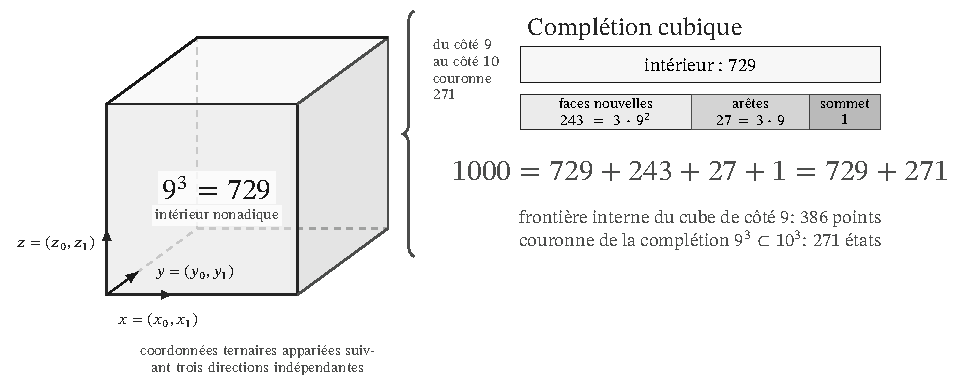
\includegraphics[width=\linewidth,keepaspectratio]{figures/cubo_emrh.pdf}
\caption{Représentation cubique de l'extension de neuf à dix classes par coordonnée. Les strates \(S_1,S_2,S_3\) placent les incidences ajoutées sur les faces, les arêtes et l'apex ; leurs cardinaux forment la couronne de \(271\) éléments. La frontière de \(386\) éléments appartient au cube initial. La perspective géométrique complète la partition de la figure ~\ref{fig:revision-emrh} ; les séparations graphiques ont une fonction schématique.}
\label{fig:completacion-cubo-recuperado}
\end{figure}

% END IX03_CUBIC_COMPLETION_FIGURE

\subsubsection{Conservation de l'unité et compatibilité dimensionnelle}

La normalisation ne se limite pas à diviser une identité isolée. En dimension
\(d\), le produit \(\widehat E^d\) porte la mesure uniforme
\(\mu_d(\{x\})=10^{-d}\). La projection coordonnée
\(p_d:\widehat E^{d+1}\to\widehat E^d\) supprime la dernière coordonnée.

\begin{proposition}[Compatibilité projective des mesures normalisées]
Pour tout \(d\geq1\),
\[
 (p_d)_*\mu_{d+1}=\mu_d,
 \qquad \mu_d(\widehat E^d)=1.
\]
La masse de la strate comportant \(r\) coordonnées supplémentaires est
\(\binom dr9^{d-r}/10^d\), et la somme des masses de toutes les strates
vaut un.
\end{proposition}
\begin{proof}
Chaque point de \(\widehat E^d\) possède dix préimages. Leur masse totale est
\(10\,10^{-(d+1)}=10^{-d}\). L'égalité pour tout sous-ensemble
s'obtient en sommant sur ses points. La formule stratifiée provient
du même dénombrement que \eqref{eq:revision-estratos} ; le binôme
\((9+1)^d\) donne la normalisation totale.
\end{proof}

En dimension trois, retirer l'apex laisse une masse \(999/1000\), et
le restituer ajoute \(1/1000\). Renormaliser avant la restitution
définirait une autre mesure : la distinction est pertinente sur le plan opératoire.
En particulier, conservation de la masse probabiliste, conservation des
registres de transport et dissipation thermodynamique sont des affirmations portant sur
des objets différents. La proposition démontre la première et fournit le
support compatible pour étudier la deuxième ; la troisième requiert une
réalisation dynamique et énergétique spécifiée.

La frontière géométrique interne demeure également distincte.
Sur le représentant cartésien \(\{1,\ldots,9\}^3\), retirer
\(\{2,\ldots,8\}^3\) laisse \(386\) points. Cette frontière appartient au
cube initial, tandis que \(\widehat C\setminus C\) appartient à son
extension. La complétion cubique, le développement positionnel en base mille et
la lecture d'incidence exceptionnelle partagent des données du support ;
leurs applications respectives déterminent l'information issue de ces données qu'utilise
chaque représentation.


% Fragmento conservado; véase MANIFIESTO_ANTECEDENTES_LECTURA.json.
% Incorporación al final de extension.tex; no contiene una sección principal.
% Procedencia: RESULTADO_RECUPERADO; explicitación sectorial de las hipótesis.
% Fuentes leídas: monografía Doble proyección holográfica (cantera editorial),
% manuscrito/local/01_tesis_recuperada.tex y
% manuscrito/generated/algebra_holonomica.tex, especialmente §§1--7 y 21.
% Definición rectora de número: manuscrito/flattened/main_autosuficiente.tex,
% secciones que comienzan en líneas 22137 y 23000 de la cantera de 775 páginas.
% No se adopta su presentación global como prueba de todas las flechas TPK.

\subsection{Le nombre comme section compatible et la valeur comme lecture}
\label{hist:seccion}

La distinction entre état et observation permet de préciser quel objet se
prolonge lorsque la résolution augmente. À la profondeur \(n\), soit \(X_n\)
l’ensemble des états admissibles produits par APP--TRIT--TPK. Leurs données
comprennent position, feuillets somme et produit, restes et quotients, régime,
orientation, retenue, phase, route, frontière, mémoire et survie. Ce ne sont pas
des coordonnées indépendantes : les évaluations arithmétiques et les transports
antérieurs imposent leurs relations. Un prolongement conserve ces relations
dans chaque antécédent, même s’il ajoute de nouvelles étapes et de nouvelles données de mémoire.
Tel est le sens de l’arithmétique des histoires développée dans
\textup{(provenance conservée dans le registre technique)}.

Soient \(r_{m,n}:X_m\to X_n\), pour \(m\geq n\), les restrictions de
profondeur, avec \(r_{n,n}=\operatorname{id}\) et
\(r_{\ell,n}=r_{m,n}\circ r_{\ell,m}\). Chaque restriction conserve le
préfixe et l’information déjà déterminée en lui.

\begin{definition}[Section numérique compatible]
Un nombre HMT est une histoire compatible du système d’états :
\begin{equation}
 x=(x_n)_{n\geq0}\in X_\infty:=\varprojlim_n X_n,
 \qquad r_{m,n}(x_m)=x_n.
 \label{hist:limite-inverso}
\end{equation}
Un lecteur est une opération supplémentaire sur un domaine spécifié de ces
histoires. Un chiffre est une observation finie ; une valeur scalaire est une
évaluation du lecteur. Le couple formé de la section et de son lecteur constitue
une présentation munie d’une lecture, non une redéfinition de l’identité de la section.
\end{definition}

Dans le domaine archimédien \(X_\infty^{\mathrm{Arch}}\), le lecteur associe
à chaque préfixe un cylindre fermé, conserve leur emboîtement et fait tendre
leur diamètre vers zéro. Il détermine ainsi
\begin{equation}
 \operatorname{ev}_{\mathbb R}:X_\infty^{\mathrm{Arch}}\longrightarrow
 \mathbb R,\qquad
 \{\operatorname{ev}_{\mathbb R}(x)\}=\bigcap_n I_n(x).
 \label{hist:evaluacion}
\end{equation}
La construction concrète de ces cylindres et la décision de leurs frontières
sont développées dans la section~\ref{sec:generacion}. La définition
\eqref{hist:limite-inverso} n’affirme pas à elle seule que l’image de
\eqref{hist:evaluacion} soit la droite entière : une affirmation de couverture
requiert son propre théorème. Une égalité de valeurs n’établit pas non plus, sans
résultat d’injectivité, l’égalité de leurs histoires. Cette séparation
permet de parler de précision comme profondeur en conservant la différence
entre l’antécédent arithmétique et sa réalisation scalaire.

\subsection{Composition des histoires et multiplicateur de mémoire}
\label{hist:algebra}

Fixons un secteur d’états à la profondeur \(n\) et une catégorie
\(\mathcal C\) dont les flèches sont leurs histoires admissibles. La composition
s’écrit \(vu=v\circ u\) : on parcourt d’abord \(u\), puis \(v\).
Les pas élémentaires proviennent de la sélection, du transport et de
l’actualisation du TPK. Une fibre tritique locale admet l’écriture
\(\mathbb R[J_x]/(J_x^2+\tau(x)1_x)\), où
\(\tau(x)\in\{+1,0,-1\}\). Le régime et l’orientation appartiennent à
l’état transporté ; une transition entre régimes n’équivaut pas à
l’identification de leurs algèbres quadratiques.

La formulation suivante précise un secteur algébrique de cette composition.
Pour chaque objet \(x\), on se donne une algèbre réelle associative unitaire \(A_x\),
éventuellement non commutative. Pour chaque \(u:x\to y\), on se donne un
homomorphisme unital \(\rho_u:A_x\to A_y\). Nous supposons une action stricte :
\begin{equation}
 \rho_{\operatorname{id}_x}=\operatorname{id}_{A_x},\qquad
 \rho_v\rho_u=\rho_{vu}.
 \label{hist:accion-estricta}
\end{equation}
Pour chaque couple composable \(u:x\to y\), \(v:y\to z\), nous fixons un
multiplicateur central inversible
\(\Omega(v,u)\in Z(A_z)^\times\). On exige la normalisation
\(\Omega(\operatorname{id}_y,u)=\Omega(u,\operatorname{id}_x)=1_y\)
et, pour chaque triplet composable, l’identité
\begin{equation}
 \rho_w\bigl(\Omega(v,u)\bigr)\Omega(w,vu)
   =\Omega(w,v)\Omega(wv,u).
 \label{hist:cociclo}
\end{equation}
Il s’agit d’hypothèses explicites sur les transports et leurs coefficients, non d’une
conséquence du qualificatif holonomique appliqué à la dynamique. Pour appliquer cette présentation
à un secteur TPK, il faut identifier ses \(\rho_u\) et \(\Omega(v,u)\).
Les transitions exprimées par des bimodules exigent la conservation de cette
structure et ne sont pas remplacées par \eqref{hist:accion-estricta}.

L’espace des sommes finies
\[
 \mathcal H(\mathcal C,A,\rho,\Omega)
   =\bigoplus_{u\in\operatorname{Mor}(\mathcal C)} A_{t(u)}T_u
\]
est muni du produit bilinéaire
\begin{equation}
 (aT_v)(bT_u)=a\rho_v(b)\Omega(v,u)T_{vu},
 \label{hist:producto}
\end{equation}
si les flèches sont composables, et de zéro sinon. Ici, \(t(u)\)
désigne l’état terminal. La somme réunit des histoires à coefficients ; le
produit concatène les histoires en conservant le multiplicateur du registre.

\begin{proposition}[Associativité sectorielle à multiplicateur central]
Sous \eqref{hist:accion-estricta} et \eqref{hist:cociclo}, le produit
\eqref{hist:producto} est associatif. Si l’ensemble des objets est fini,
son unité est \(\sum_x1_xT_{\operatorname{id}_x}\).
\end{proposition}
\begin{proof}
Pour \(u:x\to y\), \(v:y\to z\), \(w:z\to t\), soient
\(a\in A_y\), \(b\in A_z\), \(c\in A_t\). Les deux coefficients
de \(T_{wvu}\) sont
\begin{align*}
 ((cT_w)(bT_v))(aT_u):\quad&
 c\rho_w(b)\Omega(w,v)\rho_{wv}(a)\Omega(wv,u),\\
 (cT_w)((bT_v)(aT_u)):\quad&
 c\rho_w(b)\rho_w\rho_v(a)\rho_w(\Omega(v,u))\Omega(w,vu).
\end{align*}
L’action stricte identifie \(\rho_w\rho_v(a)\) à \(\rho_{wv}(a)\).
La centralité de \(\Omega(w,v)\) permet de le déplacer à droite de
ce facteur ; \eqref{hist:cociclo} égalise alors les produits restants.
Les coefficients \(a,b,c\) ne sont pas permutés. Si le triplet n’est pas composable,
les deux parenthésages sont nuls du fait de leurs états initiaux et terminaux.
La bilinéarité achève la preuve. Les identités locales et la
normalisation de \(\Omega\) vérifient l’unité indiquée.
\end{proof}

La retenue du calendrier fournit un exemple effectif. Dans la catégorie
à un objet et de flèches \(C_9\), prenons pour coefficients
\(A=\mathbb R[z,z^{-1}]\), l’action identité et
\[
 \Omega(b,a)=z^{c_0(a,b)},\qquad
 c_0(a,b)=\left\lfloor\frac{a+b}{9}\right\rfloor,
 \quad 0\leq a,b<9.
\]
Les deux sommes de retenues d’un triplet sont
\(\lfloor(a+b+c)/9\rfloor\) ; \eqref{hist:cociclo}
est donc satisfaite. La variable formelle \(z\) enregistre le tour sans
lui attribuer de valeur numérique. Imposer ensuite \(z^{12}=1\) restitue le
registre dodécaphasique du calendrier \eqref{eq:extension108} ; conserver
\(z\) sans cette relation distingue les tours successifs. L’exemple réalise
la mémoire de ce calendrier, sans l’identifier à la totalité de la
mémoire TPK.

\subsection{Double variance du raffinement et conservation de l’unité}
\label{hist:doble-varianza}

La restriction des états prolonge les observables en sens contraire.
Considérons les algèbres de fonctions, munies du produit ponctuel,
\(D_n=\operatorname{Fun}(X_n,\mathbb R)\). La précomposition définit
\begin{equation}
 r_{m,n}^*:D_n\longrightarrow D_m,
 \qquad r_{m,n}^*f=f\circ r_{m,n}.
 \label{hist:precomposicion}
\end{equation}
Ce sont des morphismes unitaux ; ils sont également injectifs lorsque les restrictions
correspondantes sont surjectives. La limite inductive
\(D_{\mathrm{cyl}}=\varinjlim_n(D_n,r_{n+1,n}^*)\) réunit les
observations de profondeur finie. Cette algèbre n’est pas identifiée ici
à l’algèbre entière des routes : prolonger les opérateurs de transport exige
également leurs compatibilités avec le raffinement.

\begin{lemma}[Unité et naturalité de l’évaluation]
Si \(e_x\) est l’indicatrice de \(x\in X_n\), on a
\begin{equation}
 r_{m,n}^*e_x=\sum_{y:\,r_{m,n}(y)=x}e_y,
 \qquad r_{m,n}^*1_n=1_m,
 \label{hist:unidad}
\end{equation}
et, pour tous \(f\in D_n\), \(y\in X_m\),
\[
 \langle r_{m,n}^*f,y\rangle=\langle f,r_{m,n}y\rangle.
\]
Chaque section \(x\in X_\infty\) détermine une évaluation bien définie
\(D_{\mathrm{cyl}}\to\mathbb R\), donnée par \([f]\mapsto f(x_n)\)
pour \(f\in D_n\).
\end{lemma}
\begin{proof}
Les fibres de \(r_{m,n}\) forment une partition de \(X_m\). Leurs
indicatrices sont orthogonales et de somme \(1_m\), ce qui démontre
\eqref{hist:unidad}. La naturalité est la définition de la précomposition.
Enfin, \((r_{m,n}^*f)(x_m)=f(x_n)\), de sorte que deux représentants
compatibles donnent la même évaluation dans la limite inductive.
\end{proof}

L’unité globale est la fonction constante un sur toutes les possibilités ;
la section individuelle sélectionne une histoire compatible. Conserver la
première ne signifie pas immobiliser la seconde. Le raffinement peut augmenter
le nombre d’extensions et la profondeur de chaque histoire en maintenant
l’unité et toutes les évaluations de ses antécédents.



\clearpage
% Fragmento conservado; véase MANIFIESTO_ANTECEDENTES_LECTURA.json.
\section{Génération coinductive de \texorpdfstring{\(\pi,\varphi,e\)}{pi, phi, e} à profondeur arbitraire}
\label{sec:generacion}

L'émission de six blocs est une étape finie de la construction, et non un développement décimal complet. Sa fonction consiste à produire des régions munies de multiplicités, d'orientations et de règles de transport. Le prolongement doit conserver ces données et déterminer une collection compatible de préfixes de longueur arbitraire. Le mot \emph{génération} désigne cette opération ; \emph{généalogie} désigne la reconstruction de ses dépendances. Les deux notions interviennent, mais remplissent des fonctions distinctes.

\subsection{Orbites, régions et caractères de clôture, de propagation et d'auto-échelle}

Sur un mot \(w=(w_1,\ldots,w_6)\), nous définissons
\[
 r(w)=(w_3,w_1,w_2,w_5,w_6,w_4),\qquad
 s(w)=(w_4,w_5,w_6,w_1,w_2,w_3).
\]
On a \(r^3=s^2=I\) et \(srs=r^{-1}\) ; ces permutations réalisent donc le groupe diédral \(D_3\). L'action conserve le catalogue et les multiplicités et commute avec \(\Psi\). Le quotient des \(243\) mots visibles possède \(43\) orbites : trente-huit de cardinal six et cinq de cardinal trois.

La classe de clôture se reconnaît par un prédicat de fibre : ses six orientations ont cinq émissions par mot, une multiplicité totale \(1008\) et une distribution \(432+4\cdot144\). Il existe une seule orbite possédant ces propriétés dans le catalogue. Pour préciser les deux autres sélections, nous écrivons \(f(w)=\#\Psi^{-1}(w)\), \(m(w)=\sum_{U\in\Psi^{-1}(w)}\operatorname{mult}(U)\) et \(\nu(w)=(n_0,n_1,n_2)\). La classe diagonale additive d'une émission est \(d(U)=[i+j]_9\) dans les indices de zéro à huit ; sa signature additive conserve cette classe et l'orientation \(ES\) ou \(NO\). Soit \(\mathcal D(\mathcal O)\) l'ensemble de ces classes pour toutes les émissions sur une orbite.

Parmi les orbites de taille six, le prédicat conjoint
\[
 f(w)=1,\qquad m(w)=144\quad(w\in\mathcal O),\qquad
 \mathcal D(\mathcal O)=\{0,3,6\}
\]
laisse exactement six orbites. Dans ce secteur, le recensement \(\nu=(2,3,1)\), égal à celui de clôture, sélectionne uniquement la propagation ; le recensement \(\nu=(2,2,2)\) sélectionne uniquement l'auto-échelle. Le support diagonal ne peut pas être omis : sans lui, il y a quatre orbites à un seul point équilibrées de multiplicité \(144\), et non une seule. Enfin, l'existence d'une émission avec \(d=6\) et une orientation \(ES\) sélectionne un représentant de chaque orbite et conduit à
\begin{equation}
 w^{\rm cl}=010211,\qquad w^{\rm pr}=201101,\qquad w^{\rm au}=121200.
 \label{eq:palabras-regionales}
\end{equation}
Ces symboles désignent d'abord des régions du catalogue. L'identification scalaire sera démontrée au moyen de leurs lecteurs ; ils ne sont pas choisis parce qu'ils coïncident avec des chiffres d'une constante connue.

Le mot de clôture \(010211\) possède les cinq préimages suivantes :
\begin{center}\small
\begin{tabular}{@{}lll r@{}}\toprule
Émission de six blocs&Signature multiplicative&Rôle&Multiplicité\\\midrule
\(501,614,498,169,272,272\)&\(555555\)&transversal&432\\
\(810,923,870,169,272,272\)&\(339555\)&orientation positive&144\\
\(810,983,810,169,272,272\)&\(393555\)&orientation positive&144\\
\(870,923,810,169,272,272\)&\(933555\)&orientation positive&144\\
\(870,923,810,418,674,521\)&\(933717\)&retour orienté&144\\\bottomrule
\end{tabular}
\end{center}
La multiplicité \(432\) et la signature constante \(555555\) caractérisent la région transversale. Elles n'identifient pas la position centrale \((5,5)\) d'APP. Confondre une signature de six fenêtres avec une position du support éliminerait la distinction entre région numérique et structure électronique.

La microfibre possède en outre une morphologie bipartite précise. Chaque émission est un produit d'une classe de curseur additif et d'une classe multiplicative. Les trois régions positives partagent la même classe additive de dix-huit conditions ; ensemble, elles contiennent trois classes multiplicatives de huit conditions chacune. La région transversale possède un produit \(18\times24\) ; les trois positives réunies, un autre \(18\times24\) ; et le retour, un produit \(18\times8\). La décomposition par émissions comporte cinq parties, tandis que la décomposition en composantes connexes du graphe biparti en comporte trois. Toutes deux conservent les mêmes \(1008\) germes sans réduire la forme à un cardinal.

\subsection{Transport fini et frontière de prolongement}

Les endomorphismes \(L_0,L_1\) de l'espace des mots ternaires agissent avant la réalisation archimédienne. Leur détermination commence par les transitions de l'état arithmétique, et non par la prescription de deux matrices. Si \(U_t\) est l'étape composée de sélection, de transport et de mise à jour, le bloc observé satisfait
\[
 b_j^\chi=\Pi_6(x_j^\chi),\qquad
 x_{j+1}^\chi=U_{9j+9}\cdots U_{9j+1}(x_j^\chi),
 \qquad \chi\in\{\mathrm{cl},\mathrm{pr},\mathrm{au}\}.
\]
On forme six transitions pour chaque régime : deux consécutives dans chacune des trois régions. Les couples de matrices d'origines et de destinations obtenus dans le registre sont
\[
\begin{array}{c|c|c|c}
X_0&Y_0&X_1&Y_1\\\hline
010211&012222&010211&002111\\
012222&010211&002111&110221\\
201101&121221&102011&012222\\
121221&102011&012222&102011\\
121200&112202&121020&010210\\
112202&121020&010210&010200
\end{array}
\]
Chaque chaîne de six chiffres représente une ligne dans \(\FF_3^6\). Puisque \(\det X_0=1\) et \(\det X_1=-1\) dans \(\FF_3\), les équations \(X_aL_a=Y_a\) déterminent de manière unique \(L_a=X_a^{-1}Y_a\). Dans cette coordinatisation par vecteurs-lignes, on obtient
\[
 L_0=\begin{pmatrix}
 2&2&2&1&2&1\\2&1&2&2&1&1\\1&0&0&1&0&2\\
 0&0&1&1&1&0\\2&2&2&0&2&1\\2&1&2&1&0&0
 \end{pmatrix},\quad
 L_1=\begin{pmatrix}
 2&1&2&0&2&2\\1&2&1&1&2&0\\1&2&1&1&1&2\\
 0&1&0&0&2&1\\2&0&2&1&0&1\\0&2&2&2&1&1
 \end{pmatrix}\quad(\bmod3).
\]
Le calendrier \((L_0,L_0,L_1,L_1)\) produit quatre nouveaux blocs de six composantes. Leurs concaténations forment
\[
 w_6\longrightarrow w_{12}\longrightarrow w_{18}
 \longrightarrow w_{24}\longrightarrow w_{30}.
\]
Les sous-indices de \(w\) indiquent la longueur accumulée. La frontière \(R_{36}\) conserve la structure terminale et ouvre la relation de prolongement ; elle n'est pas renommée comme un dernier bloc périodique qui pourrait se répéter indéfiniment.

L'identité \(L=X^{-1}Y\) démontre l'unicité une fois les transitions fixées ; elle ne remplace pas la production de ces transitions par \(U_t\). La provenance de leur registre et l'examen des seize calendriers binaires sont documentés dans le supplément technique. Le calendrier indiqué est le seul de ces seize calendriers qui reproduise conjointement les trois suites de cinq blocs.

\subsection{Cinq régions de clôture et compensation angulaire}

La région de clôture contient une composante transversale et quatre accompagnatrices. Le lecteur symétrique agit dans l'espace de leurs cinq positions au moyen de
\[
 P_5=\frac15\mathbf1\mathbf1^{\mathsf T},\qquad
 \mathbf1=(1,1,1,1,1)^{\mathsf T}.
\]
L'invariance \(P_5\lambda=\lambda\) et la conservation \(\mathbf1^{\mathsf T}\lambda=1\) imposent \(\lambda=\mathbf1/5\). Cette normalisation répartit l'unité entre les positions du lecteur ; elle ne remplace pas les multiplicités des germes \(432,144,144,144,144\) par des fréquences uniformes. La coordinatisation elliptique du lecteur réalise chaque coordonnée par \(1+\lambda_jJ\) ; sa pente est \(\lambda_j\), d'où la pente primitive \(1/5\). La règle qui fait passer d'une coordonnée normalisée à une pente est ainsi explicitée, au lieu d'identifier les deux notions sans application. Le lecteur compose les quatre positions associées selon la loi
\begin{equation}
 a\oplus b=\frac{a+b}{1-ab}.
 \label{eq:suma-pendientes}
\end{equation}
Cette loi s'obtient en multipliant \((1+aJ)(1+bJ)\) dans le régime \(J^2=-I\) et en divisant par sa composante scalaire. La composition des pentes est donc une réalisation de la structure quadratique de TRIT, et non une somme ordinaire de quatre fractions.

\begin{proposition}[Compensateur de la clôture]
La composition de quatre pentes \(1/5\) est \(120/119\). La condition de retour à une pente un détermine un unique compensateur positif de la forme \(1/q\), avec \(q>1\), et donne \(q=239\).
\end{proposition}
\begin{proof}
La première duplication donne \((1/5)\oplus(1/5)=5/12\) ; la seconde, \((5/12)\oplus(5/12)=120/119\). La condition
\[
 \frac{120/119-1/q}{1+(120/119)/q}=1
\]
équivaut à \((120-119)q=120+119\), d'où \(q=239\).
\end{proof}

Le caractère de clôture résultant a pour réalisation
\begin{equation}
 \Pi_{\rm cl}=4\left(4\arctan\frac15-\arctan\frac1{239}\right).
 \label{eq:lector-pi}
\end{equation}
L'identité angulaire de Machin reconnaît \(\Pi_{\rm cl}=\pi\). Le sens de la construction est précis : la pente et le nombre de compositions sont déclarés par le lecteur de la pentafibre ; l'équation de compensation impose \(239\). Une fois ce caractère produit, son évaluation par des séries alternées ne sélectionne pas à nouveau l'orbite des germes.

Pour \(0<x<1\), les sommes alternées
\[
 A_n(x)=\sum_{j=0}^n\frac{(-1)^jx^{2j+1}}{2j+1}
\]
encadrent \(\arctan x\) entre deux troncatures consécutives, dont la différence est \(x^{2n+3}/(2n+3)\). Appliquées aux deux pentes de \eqref{eq:lector-pi}, elles fournissent des extrémités rationnelles d'erreur explicite. La valeur numérique est ainsi calculée comme conséquence du caractère exact, sans introduire de préfixe cible.

\subsection{Lecteur de propagation et normalisation de l'unité}

La région de propagation se réalise au moyen d'une collection formelle \(P_t\in\mathcal A[[t]]\), où \(\mathcal A\) est une algèbre commutative unitaire sur \(\QQ\). Sa composition satisfait \(P_{t+s}=P_tP_s\), d'unité \(P_0=1\), et le transport élémentaire orienté fixe le générateur scalaire \(P'_0=+1\). La condition fixe son signe, et non sa seule grandeur. En écrivant
\[
 P_t=\sum_{n\ge0}a_nt^n,
\]
la normalisation détermine \(a_0=a_1=1\). La comparaison du coefficient de \(s^nt\) dans \(P_{s+t}=P_sP_t\) donne \((n+1)a_{n+1}=a_na_1\) ; de manière équivalente, \(P'_t=P_t\). Ainsi,
\begin{equation}
 (n+1)a_{n+1}=a_n,\qquad a_n=\frac1{n!}.
 \label{eq:propagacion}
\end{equation}
Le caractère en une unité de paramètre est \(\Pi_{\rm pr}=P_1\), reconnu ultérieurement comme \(e\).

La normalisation du générateur importe. La loi de semi-groupe sans cette donnée admettrait \(P_t=e^{ct}\) pour différents \(c\) ; c'est pourquoi on n'omet pas la condition qui fixe l'unité du paramètre dans le lecteur. Cette condition est antérieure à la comparaison décimale et appartient à l'exposition de la règle opératoire, et non au choix d'une valeur expérimentale.

\begin{proposition}[Bornes rationnelles de propagation]
Pour \(n\ge1\), soit \(E_n=\sum_{j=0}^n1/j!\). Alors
\[
 E_n<\Pi_{\rm pr}<E_n+\frac{n+2}{(n+1)(n+1)!}.
\]
\end{proposition}
\begin{proof}
Le premier terme omis est \(1/(n+1)!\). Chaque quotient ultérieur est au plus égal à \(1/(n+2)\). La somme géométrique majorant la queue est
\[
 \frac1{(n+1)!}\frac1{1-1/(n+2)}
 =\frac{n+2}{(n+1)(n+1)!}.
\]
L'inégalité stricte découle de la décroissance des quotients successifs.
\end{proof}

\subsection{Incidence modale et génération de l'auto-échelle}

Le sélecteur tritique produit le cycle \((+1,-1,0)\). Dans les modes \(\Sigma,\Pi\), la règle est \(+1:m\mapsto\Sigma\), \(-1:m\mapsto\Pi\), \(0:m\mapsto m\). Avec fermeture cyclique, le mode observé est \((\Sigma,\Pi,\Pi)\). Ses arêtes sont \(\Sigma\to\Pi\), \(\Pi\to\Pi\) et \(\Pi\to\Sigma\). Son incidence, dans cet ordre des modes, est donc
\begin{equation}
 F_{\rm av}=\begin{pmatrix}0&1\\1&1\end{pmatrix}.
 \label{eq:fav}
\end{equation}
Les quatre entrées s'obtiennent à partir du calendrier, et non d'une équation qui aurait préalablement reçu la valeur de \(\varphi\). La répétition du calendrier donne les dénombrements \(3F_{\rm av},9F_{\rm av},36F_{\rm av}\) aux longueurs neuf, vingt-sept et cent huit. Ces dénombrements ne sont pas les puissances de la matrice.

\begin{theorem}[Caractère positif d'auto-échelle]
L'incidence \eqref{eq:fav} possède un unique rayon propre strictement positif. En le normalisant sous la forme \((1,x)^{\mathsf T}\), sa coordonnée \(x\) satisfait \(x^2-x-1=0\), \(x>0\), et vaut \(\varphi=(1+\sqrt5)/2\).
\end{theorem}
\begin{proof}
L'équation propre donne \(x=\lambda\) et \(1+x=\lambda x\). L'élimination de \(\lambda\) produit le polynôme. Une seule de ses deux racines est positive. Comme \(F_{\rm av}^2\) a toutes ses entrées positives, le rayon positif est unique et simple. L'expression radicale reconnaît la coordonnée obtenue ; elle ne participe pas à la production de \(F_{\rm av}\).
\end{proof}

Avec \(F_0=0,F_1=1,F_{n+1}=F_n+F_{n-1}\), l'incidence induit, pour \(n\geq1\),
\[
 F_{\rm av}^n=\begin{pmatrix}F_{n-1}&F_n\\F_n&F_{n+1}\end{pmatrix}.
\]
Les quotients consécutifs \(F_{n+1}/F_n\) alternent autour de \(\varphi\). L'identité de déterminant
\[
 F_{n+1}^2-F_nF_{n+2}=(-1)^n
\]
donne une largeur exacte \(1/(F_nF_{n+1})\) entre deux quotients consécutifs. Sa croissance rend cet encadrement rationnel arbitrairement petit.

\subsection{Cylindres compatibles et profondeur arbitraire}

La réalisation d'un bloc ternaire \(b=(b_1,\ldots,b_6)\) est l'entier
\[
 \nu(b)=\sum_{j=1}^6b_j3^{6-j}\in\{0,\ldots,728\}.
\]
Une suite de blocs définit des préfixes entiers par \(N_{n+1}=729N_n+\nu(b_{n+1})\), en commençant en \(N_0=m\), où \(m\) est la partie entière déterminée par le lecteur. Les fourchettes précédentes situent les caractères de clôture, de propagation et d'auto-échelle dans \((3,4)\), \((2,3)\) et \((1,2)\), respectivement ; leurs valeurs initiales sont donc \(m=3,2,1\). Les blocs suivants raffinent la partie fractionnaire. Le cylindre correspondant est
\begin{equation}
 I_n=\left[\frac{N_n}{729^n},\frac{N_n+1}{729^n}\right],
 \qquad |I_n|=729^{-n}.
 \label{eq:cilindro}
\end{equation}
La convention semi-ouverte est utilisée pour sélectionner un représentant lorsqu'une valeur tombe sur une frontière. Pour le passage à la limite, on utilise les fermetures de ces intervalles et on identifie les deux développements de frontière équivalents. Cette précision empêche de supposer que toute intersection d'intervalles semi-ouverts emboîtés est automatiquement non vide.

\begin{theorem}[Détermination de la réalisation scalaire]
Une histoire de blocs compatible détermine une unique limite des extrémités gauches de \eqref{eq:cilindro}. Si un caractère exact dispose d'encadrements rationnels de largeur arbitrairement petite et se sépare de la frontière de chaque cylindre décimal examiné, chaque préfixe décimal de longueur finie est déterminé après un calcul fini. Les préfixes ainsi obtenus sont compatibles entre eux.
\end{theorem}
\begin{proof}
L'extension d'un bloc conserve le préfixe précédent par division euclidienne. Les cylindres fermés sont emboîtés et leur diamètre tend vers zéro ; leurs extrémités gauches forment une suite de Cauchy et possèdent une unique limite. Pour une longueur décimale fixée, une valeur séparée des frontières de la partition possède une distance positive à celles-ci. Une fourchette suffisamment étroite est contenue dans une unique cellule et détermine son préfixe. L'unicité de la cellule et l'emboîtement des partitions prouvent la compatibilité par troncature. Aux points à développement terminal, il faut ajouter la décision exacte de frontière et sa convention de représentation ; cette décision ne se déduit pas d'une largeur numérique seule.
\end{proof}

\begin{corollary}[Obtention finie et compatibilité des préfixes régionaux]
\label{gen:prefijos-regionales}
Pour chacune des réalisations \(\pi,\varphi,e\) et pour toute longueur
décimale finie, les encadrements construits déterminent le préfixe correspondant
par un calcul fini. Les préfixes obtenus à différentes profondeurs
sont compatibles par troncature.
\end{corollary}
\begin{proof}
Les caractères de clôture, de propagation et d'auto-échelle possèdent les encadrements précédents. Après leur reconnaissance, l'irrationalité de \(\pi,e,\varphi\) garantit leur séparation des frontières rationnelles de chaque partition décimale finie. On applique le théorème précédent à chaque caractère.
\end{proof}
La profondeur arbitraire exprime le quantificateur du corollaire : pour tout
horizon fini, il existe un calcul qui détermine son préfixe. L'objet
mathématique est la collection compatible complète ; chaque exécution en obtient une
projection finie.

\subsection{Involution spéculaire et synchronisation des régions}

La connexion nonadique transporte conjointement les trois caractères. Dans la coordinatisation de la neuvième phase, l'axe d'auto-échelle et la somme ternaire de clôture et de propagation restent fixés sous l'échange spéculaire. L'inversion hélicoïdale change le sens du transport ; la réflexion des deux canaux change leur orientation relative. Ce sont des involutions différentes, bien qu'elles agissent sur le même système de trajectoires.

Les coïncidences de recensement illustrent cette coordination :
\begin{center}
\begin{tabular}{@{}c rrr l@{}}\toprule
Phase&\(N_\pi\)&\(N_e\)&\(N_\varphi\)&Égalité des dénombrements\\\midrule
4&207&207&122&\(N_\pi=N_e\)\\
5&39&151&151&\(N_e=N_\varphi\)\\
6&110&110&69&\(N_\pi=N_e\)\\
7&81&29&81&\(N_\varphi=N_\pi\)\\
8&59&59&59&synchronisation triple\\
9&43&43&43&synchronisation triple\\\bottomrule
\end{tabular}
\end{center}
Ces entiers comptent des coordonnées compatibles des régions. Ils n'affirment pas une égalité entre \(\pi\), \(e\) et \(\varphi\) en tant que nombres réels. Si
\[
 \partial(a,b,c)=(a-b,b-c,c-a),
\]
son image appartient au réseau \(A_2=\{(u,v,w)\in\ZZ^3:u+v+w=0\}\). Aux phases huit et neuf, la composante relative s'annule, mais la composante diagonale passe de \((59,59,59)\) à \((43,43,43)\). La synchronisation relative coexiste avec un déplacement de \(-16\) par canal. La fermeture qui conduira à \(\alpha\) doit conserver les deux informations : coïncidence relative et évolution de la mémoire.


% Fragmento conservado; véase MANIFIESTO_ANTECEDENTES_LECTURA.json.
\subsection{Symétrie spéculaire des régions et double réalisation}
\label{mono-ampl:regiones}

L'échange spéculaire agit sur le bloc régional
\(B=(u^\pi,u^e,u^\varphi)\in(\mathbb F_3^6)^3\) par
\[
 \mathfrak cB=(u^e,u^\pi,u^\varphi).
\]
Son axe fixe et son agrégat sont respectivement \(u^\varphi\) et
\(s=u^\pi+u^e\). Cette fixation concerne l'involution dans une fibre ;
les deux coordonnées peuvent évoluer pendant le transport nonadique.
Avec \(q=u^\pi+u^e+u^\varphi\),
\(a=u^\pi+u^e-u^\varphi\) et \(d=u^\pi-u^e\), on retrouve
\[
 u^\varphi=2(q-a),\qquad s=q-u^\varphi,\qquad
 u^\pi=2(s+d),\qquad u^e=2(s-d).
\]
Les égalités sont composante par composante dans \(\mathbb F_3\), où
\(2^{-1}=2\). Le miroir conserve \(q,a,s\) et inverse \(d\) ; cette
coordonnée antisymétrique individualise la répartition que l'agrégat conserve
sans la distinguer. L'inversion \(\mathcal I\) de l'indice temporel et
l'involution \(\mathfrak c\) des canaux agissent donc sur des
données différentes.

Le retour de phase possède un témoin explicite :
\[
 \begin{aligned}
 B_1&=(012222\mid121221\mid112202),\\
 B_{10}&=(101222\mid112221\mid112002).
 \end{aligned}
\]
Les deux positions ont la phase \(1\) ; le bloc, l'axe et la mémoire ont
changé. De même, la synchronisation des dénombrements aux phases \(8\) et
\(9\) annule leurs différences relatives, tandis que la composante diagonale
passe de \((59,59,59)\) à \((43,43,43)\). L'égalité d'un observable
relatif n'épuise pas l'état qui le détermine.

La double réalisation conserve cette architecture. Dans la section 8.1 de l'Article I (provenance du corridor exceptionnel, conservée dans le registre technique), le même préfixe détermine d'une part des cylindres emboîtés et d'autre part une suite de mots codés avec leurs repères. La première application passe à la limite par contraction des diamètres ; la seconde satisfait \(r_{n,m}Q_n=Q_mp_{n,m}\) et définit \(Q_\infty\). La figure \ref{mono-ampl:fig-regional} anticipe ces deux applications. Le parcours d'incidence ultérieur construit des codes, des réseaux et la réalisation de Moonshine dans leurs domaines propres ; le groupe d'automorphismes agit sur cette réalisation, et non sur les chiffres par une identification implicite.

% Fragmento conservado; véase MANIFIESTO_ANTECEDENTES_LECTURA.json.
% Figura acumulativa; destino figures/monodromia_regional_ampliacion.tex.
\begin{figure}[!htbp]
\centering
\begin{tikzpicture}[x=1cm,y=1cm,>=Latex,font=\small,
  flow/.style={->,line width=.55pt},
  ann/.style={align=center,font=\footnotesize}]
\node[font=\bfseries] at (6.9,9.2)
  {Connexion nonadique et coordonnées régionales};
\begin{scope}[shift={(3.4,6.8)}]
 \foreach \k in {1,...,9}{
  \pgfmathsetmacro{\ang}{90-40*(\k-1)}
  \coordinate (p\k) at (\ang:1.52);
  \fill (p\k) circle (1.4pt);
  \node[fill=white,inner sep=1.1pt,font=\footnotesize]
    at (\ang:1.83) {\(\k\)};
 }
 \foreach \k in {1,...,8}{
  \pgfmathtruncatemacro{\next}{\k+1}
  \draw[flow,shorten >=3pt,shorten <=3pt] (p\k)--(p\next);
 }
 \draw[flow,shorten >=3pt,shorten <=3pt] (p9)--(p1);
 \node[ann] at (0,.1) {\(g_k\in C_9\)\\\(\Gamma_{9,k}\)};
 \node[ann] at (0,-2.23) {Un tour : \(g\mapsto g\), \(m\mapsto m+1\)};
\end{scope}
\node[ann,text width=5.25cm] at (10.1,7.75)
 {\(B_k=(u_k^\pi,u_k^e,u_k^\varphi)\)\\
 bloc régional dans une fibre};
\node at (8.55,6.5) {\(u^\pi\)};
\node at (11.65,6.5) {\(u^e\)};
\draw[<->,line width=.65pt] (8.95,6.5)--node[above]{\(\mathfrak c\)}(11.25,6.5);
\draw[densely dashed,gray] (10.1,5.72)--(10.1,7.23);
\node[fill=white,inner sep=2pt] at (10.1,5.6){\(u^\varphi\)};
\node[ann] at (10.1,4.6)
 {Axe \(u^\varphi\) et agrégat \(u^\pi+u^e\)\\
 invariants sous \(\mathfrak c\)};
\draw[flow] (5.45,6.8)--(7.25,6.8);
\draw[gray!60,line width=.3pt] (.55,4.02)--(13.25,4.02);
\node[ann,text width=12cm] (hist) at (6.9,3.47)
 {Histoire compatible : préfixes, cylindres, orientation, quotients,
 repères d'incidence et mémoire};
\coordinate (fork) at (6.9,2.85);
\draw[flow] (hist.south)--(fork);
\draw[flow] (fork)--(3.6,2.2);
\draw[flow] (fork)--(10.3,2.2);
\node[ann,text width=5.6cm] at (3.6,1.65)
 {Réalisation archimédienne\\
 \(I_{n+1}\subseteq I_n,\quad |I_n|=729^{-n}\)\\
 limite des préfixes régionaux};
\node[ann,text width=5.6cm] at (10.3,1.65)
 {Réalisation incidencielle\\
 \(r_{n,m}Q_n=Q_mp_{n,m}\)\\
 mots codés et repères compatibles};
\node[ann,text width=5.6cm] at (3.6,.42)
 {\(\pi,\varphi,e\) ; détermination dodécaphasique de \(\alpha\)};
\node[ann,text width=5.6cm] at (10.3,.42)
 {Witt--Golay--Leech--\(V^\natural\)\\
 automorphismes de la réalisation exceptionnelle};
\draw[flow] (3.6,1.03)--(3.6,.78);
\draw[flow] (10.3,1.03)--(10.3,.78);
\end{tikzpicture}
\caption{\fontsize{9}{11}\selectfont Neuf phases d'une connexion et deux réalisations de l'histoire
compatible. Le cycle représente la phase ; chaque tour incrémente le compteur.
Le diagramme régional représente l'involution \(\mathfrak c\), qui
échange clôture et propagation et fixe l'axe d'auto-échelle dans une fibre.
Cette invariance n'impose pas que l'axe reste constant pendant le transport.
Les deux applications inférieures utilisent le même préfixe : l'une détermine
sa limite numérique et l'autre conserve les mots et les cadres d'incidence. Les
applications de cette seconde réalisation sont spécifiées dans la section
8.1 de l'Article I (provenance du corridor exceptionnel, conservée dans le registre technique) ; le parcours exceptionnel est développé ensuite.}
\label{mono-ampl:fig-regional}
\end{figure}



\clearpage
% BEGIN NUCLEO_ADITIVO_20260921_SELECCION
\clearpage
% Ampliación demostrativa DF003--DF007. No modifica la fuente integral.
% Propietario común de los archivos Lean citados en estos comentarios:
% output/PAQUETE_ARTICULO_I_INTEGRACION_ESTADO_CAMPOS_20260919/.
% Residencia causal de la primera sección: después de los lectores regionales
% coinductivos y antes de emplear sus registros como entrada de la selección K.
% Residencia causal de la segunda sección: después de la construcción marcada
% Paley--Witt--Golay--Leech y antes de la reconstrucción de la estructura VOA.
% Los dos cortes expositivos conservan el mismo origen APP--TRIT--TPK.

\section[Génération régionale et raffinement]{Compatibilité intégrale de la génération régionale, du raffinement cylindrique et de l'incidence}
\label{act21:sec:df-lectores-cilindros}

La prolongation régionale produit des suites ordonnées de blocs, ainsi que
leurs profondeurs de lecture. La projection archimédienne et l'incidence
ternaire se calculent sur ces mêmes suites. Le lien entre ces deux
réalisations peut s'exprimer entièrement par des opérations entières :
sélection par intervalles rationnels, division euclidienne, élévation de six
trits, lecture de retenue et transformation de Witt. Cette formulation permet
de suivre chaque coefficient depuis son bloc générateur jusqu'à son emploi ultérieur.

La construction utilise les trois lecteurs régionaux déjà obtenus de l'état APP--TRIT--TPK. Nous les désignerons par les indices \(c\in\{\mathrm P,\mathrm E,\mathrm F\}\), correspondant respectivement aux régions de clôture, de propagation et d'auto-échelle. Leur réalisation réelle s'écrira \(v_c\). Les identifications ultérieures \(v_{\mathrm P}=\pi_{\mathrm{HMT}}\), \(v_{\mathrm E}=e_{\mathrm{HMT}}\) et \(v_{\mathrm F}=\varphi_{\mathrm{HMT}}\) conservent cet ordre causal. L'opération qui émet un bloc inspecte les intervalles rationnels du lecteur régional ; la valeur réelle intervient dans la démonstration de correction de cette opération.

\subsection{Émission positionnelle par séparation rationnelle de cellules}
\label{act21:subsec:df-emision-racional}

% Fuente: lean/biblioteca/RegionalPublicationComposition.lean,
% produced_brackets, eventual_publication, joint_eventual_publication,
% search_terminates, stopped_cell_correct, publications_compatible.

Pour chaque région, on dispose de deux suites rationnelles
\(\ell_c(j),u_c(j)\), construites par son lecteur, qui satisfont
\[
 \ell_c(j)\leq v_c\leq u_c(j).
\]
La propriété de séparation des cellules démontrée pour ces lecteurs affirme
que, pour chaque entier \(s>0\), il existe \(J\) tel que, pour tout \(j\geq J\),
\begin{equation}
 \lfloor s\ell_c(j)\rfloor
 =\lceil su_c(j)\rceil-1
 =\lfloor sv_c\rfloor.
 \label{act21:eq:df-separacion-celdas}
\end{equation}
L'évitement des frontières rationnelles par les valeurs régionales est l'hypothèse des théorèmes précédents qui garantit cette séparation. Ici, on emploie sa conclusion opérationnelle, avec les lecteurs et les intervalles qui la produisent.

\begin{definition}[Indice de séparation et préfixe émis]
Pour \(s>0\), soit
\[
 j_c(s)=\min\{j\in\mathbb N:
 \lfloor s\ell_c(j)\rfloor=\lceil su_c(j)\rceil-1\}.
\]
Pour une base entière \(b\geq2\) et une profondeur \(n\geq0\), on définit
\begin{equation}
 P_c(b,n)=\lfloor b^n\ell_c(j_c(b^n))\rfloor.
 \label{act21:eq:df-publicacion-prefijo}
\end{equation}
Le préfixe contient la partie entière et les premières \(n\) positions en base \(b\) ; par conséquent, \(P_c(b,0)\) est la partie entière régionale.
\end{definition}

\begin{theorem}[Terminaison et correction de l'émission]
\label{act21:thm:df-emision-correcta}
L'indice \(j_c(s)\) existe pour tout \(s>0\). Les préfixes émis satisfont
\begin{equation}
 P_c(b,n)=\lfloor b^n v_c\rfloor,
 \qquad
 P_c(b,n)\leq b^n v_c<P_c(b,n)+1.
 \label{act21:eq:df-prefijo-correcto}
\end{equation}
Pour chaque échelle \(s\) il est possible en outre de choisir un unique indice de suffisance \(J(s)\) valide simultanément pour les trois régions.
\end{theorem}

\begin{proof}
L'égalité à partir d'un certain rang de \eqref{act21:eq:df-separacion-celdas} rend non vide
l'ensemble qui définit \(j_c(s)\). Son minimum existe par le bon ordre de
\(\mathbb N\). À tout indice où l'égalité se produit, la borne
inférieure rationnelle fournit
\(\lfloor s\ell_c(j)\rfloor\leq\lfloor sv_c\rfloor\).
La borne supérieure, jointe à l'évitement d'une frontière de cellule, donne
\(\lfloor sv_c\rfloor\leq\lceil su_c(j)\rceil-1\).
Les deux extrémités entières coïncidant, l'entier intermédiaire coïncide avec
elles. Cela démontre \eqref{act21:eq:df-prefijo-correcto}. Pour l'affirmation
conjointe, il suffit de prendre le maximum des trois indices de suffisance obtenus
pour la même échelle. L'indice conjoint contrôle simultanément les trois
émissions, tandis que chaque région conserve ses propres intervalles.
\end{proof}

\begin{proposition}[Compatibilité exacte des préfixes]
\label{act21:prop:df-prefijos-compatibles}
Pour \(n,m\geq0\),
\begin{equation}
 \left\lfloor\frac{P_c(b,n+m)}{b^m}\right\rfloor=P_c(b,n).
 \label{act21:eq:df-truncamiento}
\end{equation}
En particulier, le bloc suivant
\(d_c(b,n)=P_c(b,n+1)\bmod b\) satisfait
\begin{equation}
 P_c(b,n+1)=bP_c(b,n)+d_c(b,n),\qquad 0\leq d_c(b,n)<b.
 \label{act21:eq:df-paso-posicional}
\end{equation}
\end{proposition}

\begin{proof}
Écrivons \(b^n v_c=N+\theta\), avec
\(N=P_c(b,n)\) et \(0\leq\theta<1\). Alors
\(P_c(b,n+m)=b^mN+\lfloor b^m\theta\rfloor\), et le second terme
appartient à \(\{0,\ldots,b^m-1\}\). La division euclidienne par \(b^m\)
récupère \(N\). La spécialisation \(m=1\) produit
\eqref{act21:eq:df-paso-posicional} et sa borne résiduelle.
\end{proof}

\subsection{Blocs régionaux de six trits à profondeur arbitraire}
\label{act21:subsec:df-bloques-arbitrarios}

% Fuente: deltas/integracion/JointRegionalFrontier.lean,
% publish_base729_eq_base3, generated_block_from_longer_prefix,
% generated_block_eq_finite, generated_signature_eq_finite.

L'égalité entière \(729=3^6\) détermine le regroupement de six positions ternaires en un bloc. Pour \(t\geq0\), nous définissons
\begin{equation}
 u_c(t)=P_c(729,t+1)\bmod729,
 \qquad
 B_{c,j}(t)=
 \left\lfloor\frac{u_c(t)}{3^{5-j}}\right\rfloor\bmod3,
 \quad 0\leq j<6.
 \label{act21:eq:df-bloque-y-banda}
\end{equation}
Ainsi, \(B_c(t)\) est un mot ordonné de six trits et
\begin{equation}
 u_c(t)=\sum_{j=0}^{5}B_{c,j}(t)3^{5-j}.
 \label{act21:eq:df-elevacion-banda}
\end{equation}
Le mot et son élévation entière sont deux représentations mutuellement récupérables du même bloc émis.

\begin{theorem}[Stabilité d'extraction à toute profondeur]
\label{act21:thm:df-bloque-estable}
On vérifie, pour tout \(n\),
\[
 P_c(729,n)=P_c(3,6n).
\]
Si \(t<n\), alors
\begin{equation}
 u_c(t)=
 \left\lfloor\frac{P_c(729,n)}{729^{n-t-1}}\right\rfloor\bmod729.
 \label{act21:eq:df-bloque-prefijo-largo}
\end{equation}
En conséquence, toute extension du préfixe préserve tous les
blocs précédemment émis et toutes les signatures calculées dessus.
\end{theorem}

\begin{proof}
La première égalité résulte de ce que les deux préfixes se séparent à la même
échelle, \(729^n=3^{6n}\), et du
théorème~\ref{act21:thm:df-emision-correcta}. Pour la seconde, nous appliquons
\eqref{act21:eq:df-truncamiento} aux profondeurs \(n\) et \(t+1\), puis
nous prenons le résidu modulo \(729\). L'extraction ternaire de
\eqref{act21:eq:df-bloque-y-banda} est déterministe. Toute fonction explicite
de ces dix-huit coordonnées conserve, par conséquent, le même résultat en
étendant le préfixe.
\end{proof}

La construction est quantifiée sur \(t\in\mathbb N\). Une table qui
matérialise cent blocs constitue une évaluation finie de cette
construction ; la formule \eqref{act21:eq:df-bloque-prefijo-largo} détermine
exactement sa compatibilité avec toute extension ultérieure.

\begin{example}[Premier bloc conjoint]
L'évaluation des lecteurs régionaux sélectionnés donne les mots
\[
 B_{\mathrm P}(0)=010211,\qquad
 B_{\mathrm E}(0)=201101,\qquad
 B_{\mathrm F}(0)=121200.
\]
Leur élévation par \eqref{act21:eq:df-elevacion-banda} produit
\[
 u_{\mathrm P}(0)=103,\qquad
 u_{\mathrm E}(0)=523,\qquad
 u_{\mathrm F}(0)=450.
\]
Par exemple,
\(201101_3=2\cdot243+27+9+1=523\).
Les six positions, y compris les zéros initiaux, sont conservées dans la
représentation en bande. Le zéro initial de \(010211\) possède une position
définie, bien que l'écriture décimale de \(103\) en soit dépourvue.
\end{example}

\subsection{Registres de transition et reconstruction des élévations linéaires}
\label{act21:subsec:df-registros-transicion}

% Fuentes: deltas/integracion/RegionalTransitionRecords.lean y
% GeneratedTransitionRecords.lean; lean/biblioteca/TPKLifts.lean.
% Los enlaces reconstruidos son R(0)->R(1) y R(2)->R(3).

Sur \(\mathbb F_3\), nous réunissons deux émissions consécutives de chaque région dans la matrice
\begin{equation}
 R(t)=
 \begin{pmatrix}
 B_{\mathrm P}(t)\\ B_{\mathrm P}(t+1)\\
 B_{\mathrm E}(t)\\ B_{\mathrm E}(t+1)\\
 B_{\mathrm F}(t)\\ B_{\mathrm F}(t+1)
 \end{pmatrix}.
 \label{act21:eq:df-registro-matricial}
\end{equation}
Cette définition fixe à la fois l'ordre régional et l'ordre temporel. Les
quatre premiers registres sont
\[
 X_0=R(0),\quad Y_0=R(1),\quad X_1=R(2),\quad Y_1=R(3).
\]
Ses valeurs, obtenues par extraction des préfixes régionaux, sont
\begin{align*}
 X_0&=\begin{pmatrix}
0&1&0&2&1&1\\0&1&2&2&2&2\\2&0&1&1&0&1\\
1&2&1&2&2&1\\1&2&1&2&0&0\\1&1&2&2&0&2
\end{pmatrix},&
 Y_0&=\begin{pmatrix}
0&1&2&2&2&2\\0&1&0&2&1&1\\1&2&1&2&2&1\\
1&0&2&0&1&1\\1&1&2&2&0&2\\1&2&1&0&2&0
\end{pmatrix},\\[1ex]
 X_1&=\begin{pmatrix}
0&1&0&2&1&1\\0&0&2&1&1&1\\1&0&2&0&1&1\\
0&1&2&2&2&2\\1&2&1&0&2&0\\0&1&0&2&1&0
\end{pmatrix},&
 Y_1&=\begin{pmatrix}
0&0&2&1&1&1\\1&1&0&2&2&1\\0&1&2&2&2&2\\
1&0&2&0&1&1\\0&1&0&2&1&0\\0&1&0&2&0&0
\end{pmatrix}.
\end{align*}

\begin{theorem}[Reconstruction unique des deux liens initiaux]
\label{act21:thm:df-elevaciones-reconstruidas}
Les équations \(X_0L_0=Y_0\) et \(X_1L_1=Y_1\) ont, chacune, une
unique solution dans \(M_6(\mathbb F_3)\). Ces solutions sont
\begin{align*}
 L_0&=\begin{pmatrix}
2&2&2&1&2&1\\2&1&2&2&1&1\\1&0&0&1&0&2\\
0&0&1&1&1&0\\2&2&2&0&2&1\\2&1&2&1&0&0
\end{pmatrix},&
 L_1&=\begin{pmatrix}
2&1&2&0&2&2\\1&2&1&1&2&0\\1&2&1&1&1&2\\
0&1&0&0&2&1\\2&0&2&1&0&1\\0&2&2&2&1&1
\end{pmatrix}.
\end{align*}
Les deux matrices sont inversibles.
\end{theorem}

\begin{proof}
Les matrices
\begin{align*}
 A_0&=\begin{pmatrix}
1&1&2&0&1&2\\0&0&1&0&0&1\\2&1&2&1&0&1\\
0&2&0&1&0&2\\2&1&1&0&2&2\\2&1&1&1&1&2
\end{pmatrix},&
 A_1&=\begin{pmatrix}
1&0&1&2&0&0\\0&0&1&1&2&2\\0&1&2&0&1&1\\
1&1&0&2&0&0\\1&1&2&1&1&2\\1&0&0&0&0&2
\end{pmatrix}
\end{align*}
satisfont \(A_iX_i=X_iA_i=I\), par multiplication dans \(\mathbb F_3\).
Par conséquent, les solutions sont imposées par \(L_i=A_iY_i\) ; la
multiplication produit les deux matrices montrées. Leurs inverses sont
\begin{align*}
 L_0^{-1}&=\begin{pmatrix}
1&2&0&2&0&2\\2&0&2&2&0&0\\2&1&2&0&2&0\\
1&0&0&0&2&0\\0&2&1&1&2&0\\2&2&2&2&2&2
\end{pmatrix},&
 L_1^{-1}&=\begin{pmatrix}
2&0&2&1&2&1\\2&1&0&0&2&0\\2&0&2&2&0&2\\
2&0&0&1&1&0\\1&1&1&1&1&0\\2&0&1&2&2&0
\end{pmatrix}.
\end{align*}
La vérification bilatérale \(L_iL_i^{-1}=L_i^{-1}L_i=I\) démontre la
récupération exacte de chaque mot transformé. Tous les produits
utilisent des résidus \(0,1,2\), avec leur interprétation en \(\mathbb F_3\).
\end{proof}

La lecture causale de ce résultat est précise : les émissions régionales produisent \(R(t)\) ; les registres \(R(0),\ldots,R(3)\) déterminent les deux élévations précédentes ; leurs inverses récupèrent les mots transformés.  
La continuité pour tout \(t\) appartient aux lecteurs coinductifs et au théorème ~\ref{act21:thm:df-bloque-estable}. La reconstruction matricielle démontrée ici a pour domaine les deux liens spécifiés dans son énoncé.

\subsection{Raffinement simultané dans les bases ternaire et décimale}
\label{act21:subsec:df-cilindros-mixtos}

% Fuente: deltas/integracion/RegionalCylinderTransition.lean.

Une émission ternaire de six trits et une émission décimale de trois chiffres
constituent deux lectures de bases différentes. Pour conserver leur relation, on
enregistre l'état
\[
 s=(n,k,N,D),
\]
où \(N\) est un préfixe de profondeur \(n\) en base \(729\), et \(D\) est
un préfixe de profondeur \(k\) en base \(1000\). Leurs cylindres
archimédiens sont
\begin{equation}
 I_{729}(s)=\left[\frac{N}{729^n},\frac{N+1}{729^n}\right),\qquad
 I_{1000}(s)=\left[\frac{D}{1000^k},\frac{D+1}{1000^k}\right).
 \label{act21:eq:df-cilindros}
\end{equation}
L'extrémité supérieure semi-ouverte attribue chaque valeur à une unique cellule d'une base et d'une profondeur données.

\begin{definition}[Défauts entiers de compatibilité]
On définit
\begin{align}
 A(s)&=N1000^k-D729^n,\label{act21:eq:df-defecto-inferior}\\
 B(s)&=(N+1)1000^k-D729^n=A(s)+1000^k.
 \label{act21:eq:df-defecto-superior}
\end{align}
L'état est compatible lorsque
\begin{equation}
 A(s)<729^n,\qquad B(s)>0.
 \label{act21:eq:df-compatibilidad}
\end{equation}
\end{definition}

\begin{lemma}[Critère entier d'intersection]
Les cylindres de \eqref{act21:eq:df-cilindros} ont une intersection non vide si et
seulement si \eqref{act21:eq:df-compatibilidad} est vérifiée.
\end{lemma}

\begin{proof}
Deux intervalles semi-ouverts \([a,b)\) et \([c,d)\), avec \(a<b\) et
\(c<d\), se coupent exactement lorsque \(a<d\) et \(c<b\). En appliquant cette
condition à \eqref{act21:eq:df-cilindros} et en multipliant par les dénominateurs
positifs, nous obtenons
\(N1000^k<(D+1)729^n\) et
\(D729^n<(N+1)1000^k\). Ce sont les deux inégalités de
\eqref{act21:eq:df-compatibilidad}.
\end{proof}

\begin{definition}[Mise à jour des profondeurs et des préfixes]
Pour \(0\leq u<729\) et \(0\leq d<1000\), nous définissons
\begin{align*}
 T_u(n,k,N,D)&=(n+1,k,729N+u,D),\\
 T_{u,d}(n,k,N,D)&=(n+1,k+1,729N+u,1000D+d).
\end{align*}
La première opération raffine uniquement le cylindre ternaire. La seconde  
raffine les deux lectures et conserve les deux profondeurs dans l'état.
\end{definition}

\begin{proposition}[Récurrences exactes de frontière]
\label{act21:prop:df-rec-frontera}
Les mises à jour précédentes satisfont
\begin{align}
 A(T_u s)&=729A(s)+u1000^k,\label{act21:eq:df-rec-ternaria}\\
 A(T_{u,d}s)&=729000A(s)+u1000^{k+1}-d729^{n+1}.
 \label{act21:eq:df-rec-conjunta}
\end{align}
\end{proposition}

\begin{proof}
Pour la première identité,
\[
 (729N+u)1000^k-D729^{n+1}
 =729(N1000^k-D729^n)+u1000^k.
\]
Pour la seconde,
\begin{align*}
 &(729N+u)1000^{k+1}-(1000D+d)729^{n+1}\\
 &\qquad=729000(N1000^k-D729^n)
      +u1000^{k+1}-d729^{n+1}.
\end{align*}
Les deux sont des identités entières antérieures à toute approximation réelle.
\end{proof}

\begin{theorem}[Raffinement des cylindres régionaux générés]
\label{act21:thm:df-refinamiento-generado}
Soit
\[
 s_c(n,k)=(n,k,P_c(729,n),P_c(1000,k)).
\]
Alors \(s_c(n,k)\) est compatible quels que soient \(n,k\). De plus,
\begin{align*}
 T_{u_c(n)}s_c(n,k)&=s_c(n+1,k),\\
 T_{u_c(n),d_c(1000,k)}s_c(n,k)&=s_c(n+1,k+1).
\end{align*}
La division euclidienne des préfixes raffinés récupère exactement les
préfixes précédents. Pour tout \(a,b\geq0\),
\[
 \frac{P_c(729,n+a)-P_c(729,n+a)\bmod729^a}{729^a}
 =P_c(729,n),
\]
et l'identité analogue est vérifiée en base \(1000\).
\end{theorem}

\begin{proof}
Le théorème~\ref{act21:thm:df-emision-correcta} place \(v_c\) simultanément dans
les deux intervalles \eqref{act21:eq:df-cilindros} ; le critère d'intersection donne
la compatibilité. Les identités de mise à jour sont
\eqref{act21:eq:df-paso-posicional} dans chaque base. La récupération s'obtient à partir de
\eqref{act21:eq:df-truncamiento}. Par conséquent, la récurrence du défaut et la
récupération du préfixe sont des conséquences d'une même mise à jour.
\end{proof}

\begin{example}[Premier couple de cylindres régionaux]
Pour \(n=k=1\), l'évaluation des trois régions donne
\[
\begin{array}{c|rr|rr}
 c&N&D&A&B\\\hline
 \mathrm P&2290&3141&211&1211\\
 \mathrm E&1981&2718&-422&578\\
 \mathrm F&1179&1618&-522&478
\end{array}
\]
Dans les trois lignes \(A<729\) et \(B>0\). La première colonne de préfixes
se décompose comme \(2290=3\cdot729+103\),
\(1981=2\cdot729+523\) et \(1179=729+450\) : réapparaissent exactement les
blocs de six trits déjà émis. Les signes différents de \(A\) expriment
la position relative des deux extrémités inférieures, sans altérer la
appartenance commune de la valeur régionale.
\end{example}

\subsection{Sélection du bloc suivant par le lecteur régional}

La compatibilité de deux intervalles exprime une relation entre lectures. La détermination du bloc suivant utilise en outre l'intervalle rationnel produit par la région. Cette opération peut se formuler sans éliminer l'histoire de profondeur.

\begin{definition}[Admissibilité de la prolongation régionale]
\(c,n\) étant fixés, soient \(s=729^{n+1}\) et \(j=j_c(s)\). Un résidu
\(u\in\{0,\ldots,728\}\) est admissible lorsque
\begin{equation}
 \lfloor s\ell_c(j)\rfloor
 \leq729P_c(729,n)+u
 \leq\lceil su_c(j)\rceil-1.
 \label{act21:eq:df-admisibilidad}
\end{equation}
\end{definition}

\begin{theorem}[Unicité de la prolongation compatible avec le lecteur]
\label{act21:thm:df-prolongacion-unica}
La condition \eqref{act21:eq:df-admisibilidad} est équivalente à \(u=u_c(n)\).
Par conséquent, il existe exactement une prolongation admissible de chaque région
à chaque profondeur.
\end{theorem}

\begin{proof}
À l'indice de séparation, les deux extrémités entières de
\eqref{act21:eq:df-admisibilidad} coïncident avec \(P_c(729,n+1)\).
La condition est ainsi équivalente à
\(729P_c(729,n)+u=P_c(729,n+1)\).
Par \eqref{act21:eq:df-paso-posicional}, le côté droit est
\(729P_c(729,n)+u_c(n)\). L'annulation du terme commun donne l'égalité des résidus. Réciproquement, cette égalité satisfait la condition.
\end{proof}

La dépendance effective de cette sélection reste complètement déterminée :
région sélectionnée, lecteur rationnel, profondeur, indice de séparation,
préfixe antérieur et résidu suivant. Le défaut \(A\) résume une relation
de frontière ; l'état \((n,k,N,D)\) et les intervalles régionaux conservent
les données employées par la mise à jour.

\subsection{Signature ternaire, retenue, incidence de Witt et horloge de lecture}
\label{act21:subsec:df-firma-conjunta}

% Fuentes: lean/regional/N69RegionalSignature.lean,
% deltas/integracion/JointRegionalFrontier.lean y JointCylinderSignature.lean.

Une profondeur \(t\) étant fixée, écrivons \(B_{c,j}=B_{c,j}(t)\). Pour chaque colonne \(j\), on calcule les entiers et les résidus suivants :
\begin{align}
 S_j&=B_{\mathrm P,j}+B_{\mathrm E,j}+B_{\mathrm F,j},
 &q_j&=S_j\bmod3,
 &c_j&=\left\lfloor S_j/3\right\rfloor,
 \label{act21:eq:df-firma-qc}\\
 a_j&=(B_{\mathrm P,j}+B_{\mathrm E,j}-B_{\mathrm F,j})\bmod3,
 &w_j&=\sum_c\mathbf1_{B_{c,j}\ne0},
 &\bar w_j&=w_j\bmod3.
 \label{act21:eq:df-firma-axial}
\end{align}
Le résidu de l'expression axiale est pris dans les entiers. Une implémentation
avec des naturels le calcule comme
\((B_{\mathrm P,j}+B_{\mathrm E,j}+3-B_{\mathrm F,j})\bmod3\), qui le conserve
exactement.

La matrice d'incidence ternaire utilisée par le lecteur est
\begin{equation}
 W=\begin{pmatrix}
0&1&1&1&1&1\\
1&0&1&1&2&2\\
1&1&0&2&1&2\\
1&1&2&0&2&1\\
1&2&1&2&0&1\\
1&2&2&1&1&0
\end{pmatrix}.
\label{act21:eq:df-matriz-witt}
\end{equation}
Pour chaque région, deux charges résiduelles sont conservées :
\begin{equation}
 v_c^{\mathrm{res}}=\sum_j B_{c,j}\bmod3,
 \qquad
 v_c^{\mathrm W}=\sum_j(B_cW)_j\bmod3.
 \label{act21:eq:df-cargas-residuales}
\end{equation}
La signature complète du lecteur est
\(\mathcal S(B)=(q,a,c,w,\bar w,v^{\mathrm{res}},v^{\mathrm W})\).
Sa structure conserve séparément le reste de colonne, la retenue, le
contraste axial, le poids de support et les deux lectures de charge.

\begin{theorem}[Récupération exacte et bornes de la signature]
\label{act21:thm:df-recuperacion-firma}
Pour chaque colonne et chaque région, on a
\begin{align}
 S_j&=q_j+3c_j,&0\leq q_j,a_j&<3,&0\leq c_j&\leq2,
 \label{act21:eq:df-recuperacion-total}\\
 B_{\mathrm F,j}&=2(q_j+3-a_j)\bmod3,&0\leq w_j&\leq3,
 &0\leq\bar w_j&<3.
 \label{act21:eq:df-recuperacion-eje}
\end{align}
De plus,
\begin{equation}
 v_c^{\mathrm W}
 =\left(\sum_j\bigl((B_cW)_j\bmod3\bigr)\right)\bmod3.
 \label{act21:eq:df-witt-reduccion}
\end{equation}
Les récupérations énoncées déterminent le total de chaque colonne et sa
coordonnée d'auto-échelle ; le registre régional conserve en outre
les trois bandes ordonnées.
\end{theorem}

\begin{proof}
L'identité \eqref{act21:eq:df-recuperacion-total} est la division euclidienne de
\(S_j\) par \(3\). Chaque terme de \(S_j\) est entre \(0\) et \(2\),
de telle sorte que \(0\leq S_j\leq6\) et \(c_j\leq2\). En \(\mathbb F_3\),
la soustraction des deux congruences qui définissent \(q_j\) et \(a_j\) donne
\(q_j-a_j=2B_{\mathrm F,j}\). Comme l'inverse de \(2\) est \(2\), on
obtient \eqref{act21:eq:df-recuperacion-eje} ; le terme \(3\) permet
d'écrire celle-ci avec des nombres naturels. Les bornes de \(w_j\) résultent de sommer trois
indicateurs. Enfin, réduire une somme entière modulo \(3\) équivaut
à réduire chaque terme et à réduire à nouveau la somme, ce qui prouve
\eqref{act21:eq:df-witt-reduccion}.
\end{proof}

\begin{example}[Signature du premier bloc conjoint]
Les trois bandes initiales produisent
\begin{align*}
 q&=(0,0,2,2,1,2),&a&=(1,2,0,1,1,2),\\
 c&=(1,1,0,1,0,0),&w&=(2,2,2,3,1,2),\\
 v^{\mathrm{res}}&=(2,2,0),&v^{\mathrm W}&=(2,1,1).
\end{align*}
La quatrième colonne a un total \(2+1+2=5\) ; sa signature enregistre \(q_3=2\) et \(c_3=1\), par conséquent \(q_3+3c_3=5\).
La récupération axiale donne \(2(2+3-1)\bmod3=2\), précisément la coordonnée d'auto-échelle.
Les images de Witt, réduites composante par composante, sont
\[
 (2,0,2,1,1,2),\qquad
 (0,0,0,2,0,2),\qquad
 (2,1,1,2,1,0).
\]
Sa somme résiduelle par ligne produit les trois charges \((2,1,1)\).
\end{example}

\begin{definition}[Horloge entière de lecture décimale]
L'indice de transition \(t\) et la profondeur décimale de représentation sont
reliés par
\begin{equation}
 \kappa(t)=\max\{k\in\mathbb N:1000^k\leq3^{6(t+1)}\}.
 \label{act21:eq:df-reloj}
\end{equation}
\end{definition}

\begin{proposition}[Caractérisation et monotonie de l'horloge]
\label{act21:prop:df-reloj}
L'entier \(\kappa(t)\) est déterminé de manière univoque par
\begin{equation}
 1000^{\kappa(t)}\leq729^{t+1}<1000^{\kappa(t)+1}.
 \label{act21:eq:df-reloj-cotas}
\end{equation}
La fonction \(\kappa\) est monotone et satisfait
\(\kappa(20)=\kappa(21)=20\).
\end{proposition}

\begin{proof}
Les puissances de \(1000\) sont strictement croissantes et non bornées ;
il existe donc un unique intervalle de puissances consécutives qui
contient \(729^{t+1}\). La monotonie de cette dernière expression démontre
celle de \(\kappa\). Les deux évaluations finales sont les comparaisons
entières
\[
 1000^{20}\leq729^{21}<1000^{21},\qquad
 1000^{20}\leq729^{22}<1000^{21}.
\]
Ces comparaisons s'effectuent avec des puissances entières exactes.
\end{proof}

L'égalité de profondeur décimale en deux transitions distinctes explique la nécessité de conserver les deux indices : l'horloge de lecture peut rester constante tandis que la bande ternaire avance et que sa signature est mise à jour. L'information chronologique se trouve dans le registre ordonné des transitions.

\subsection{Théorème de composition du bloc, du cylindre et de la signature}

\begin{theorem}[Compatibilité conjointe des lectures régionales]
\label{act21:thm:df-composicion-conjunta}
Pour chaque profondeur \(n\), il existe un unique triplet de blocs
\((u_{\mathrm P},u_{\mathrm E},u_{\mathrm F})\) qui satisfait
l'admissibilité régionale \eqref{act21:eq:df-admisibilidad} dans les trois régions.
Ce triplet est \((u_{\mathrm P}(n),u_{\mathrm E}(n),u_{\mathrm F}(n))\).
Simultanément :
\begin{enumerate}
\item chaque bloc met à jour son cylindre par les récurrences
\eqref{act21:eq:df-rec-ternaria} et \eqref{act21:eq:df-rec-conjunta} ;
\item ses six trits produisent la signature
\(\mathcal S(B_{\mathrm P}(n),B_{\mathrm E}(n),B_{\mathrm F}(n))\);
\item les totaux de colonne se retrouvent comme \(q+3c\), et les charges de Witt sont obtenues à partir des mêmes bandes par
\eqref{act21:eq:df-witt-reduccion} ;
\item tout préfixe de plus grande profondeur renvoie exactement ces
blocs, cylindres tronqués et signatures.
\end{enumerate}
\end{theorem}

\begin{proof}
Nous appliquons le théorème ~\ref{act21:thm:df-prolongacion-unica} à chacun des trois
indices régionaux. L'unicité coordonnée par coordonnée donne l'unicité
conjointe. Nous substituons ces mêmes résidus dans les opérations
\(T_u,T_{u,d}\), ce qui permet d'appliquer le
théorème ~\ref{act21:thm:df-refinamiento-generado}. L'application déterministe de
\eqref{act21:eq:df-bloque-y-banda} produit les bandes utilisées par
\eqref{act21:eq:df-firma-qc}--\eqref{act21:eq:df-cargas-residuales}. Les identités
de récupération sont celles du théorème ~\ref{act21:thm:df-recuperacion-firma}.
Finalement, le théorème ~\ref{act21:thm:df-bloque-estable} et le troncage de
chaque base démontrent la stabilité à plus grande profondeur. À chaque étape, on a conservé l'identité du bloc émis ; aucune des deux
lectures ne requiert de sélectionner un autre bloc.
\end{proof}

La conclusion est une compatibilité opérationnelle entre la contraction
cylindrique et la conservation de l'incidence. Les deux utilisent le même
registre généré, maintiennent les profondeurs et admettent la récupération
entière. Ce résultat est la forme explicite du lien
\[
 \text{bloc régional émis}
 \longrightarrow
 \begin{cases}
 \text{cylindre et frontière entière},\\
 \text{bande, signature, retenue et charge de Witt}.
 \end{cases}
\]
Le développement ultérieur de l'incidence et des champs emploie la deuxième lecture, conservant l'origine commune avec la première.

\subsection{Recensement des calendriers et compatibilité simultanée des biographies régionales}
Les lignes précédentes se regroupent, sans appliquer encore aucun lecteur décimal,
dans les trois biographies de blocs produites par les transitions :
\begin{align}
 B^{\rm cl}
  &=010211|012222|010211|002111|110221,\notag\\
 B^{\rm pr}
  &=201101|121221|102011|012222|102011,
 \label{act21:eq:biografias-tpk-tres-caracteres}\\
 B^{\rm au}
  &=121200|112202|121020|010210|010200.\notag
\end{align}
En effet, les paires consécutives des deux premiers tronçons sont les lignes de \(X_0,Y_0\), et celles des deux derniers sont les lignes de \(X_1,Y_1\). Ainsi, les biographies sont une autre écriture du registre de douze transitions, non une collection de préfixes conventionnels.

Pour vérifier le mot opératoire du calendrier, soit
\(c=c_1c_2c_3c_4\in\{0,1\}^4\) et, pour chaque régime
\(\chi\in\{{\rm cl},{\rm pr},{\rm au}\}\), définissons
\[
 u_0^\chi=b_0^\chi,\qquad
 u_j^\chi=u_{j-1}^\chi L_{c_j}\quad(1\le j\le4).
\]
Pour condenser le recensement, notons par
\[
 N_{\mathrm{ar}}(c):=
 \#\{(j,\chi):u_j^\chi=b_j^\chi,\ 1\le j\le4\},\qquad
 N_{\mathrm{bio}}(c):=
 \#\{\chi:(u_0^\chi,\ldots,u_4^\chi)=B^\chi\}.
\]
La multiplication exacte dans \(\FF_3\) des seize calendriers donne :
\[
\begin{array}{c|c|c}
 c&N_{\mathrm{ar}}(c)&N_{\mathrm{bio}}(c)\\ \hline
0000,0001&6&0\\
0010&9&0\\
0011&12&3\\
0100,0101,0110,0111&3&0\\
1000,1001,1010,1011&0&0\\
1100,1101,1110,1111&0&0
\end{array}
\tag{D}
\label{act21:eq:censo-dieciseis-calendarios}
\]
Le tableau épuise les \(2^4=16\) possibilités et chacune de ses entrées s'obtient
par quatre multiplications d'une ligne par l'une des deux matrices reproduites.
Par conséquent, \(0011\) est l'unique calendrier qui reconstruit
simultanément les trois biographies complètes. En notation opératorielle,
\begin{equation}
 (L_0,L_0,L_1,L_1)
 \label{act21:eq:calendario-0011-interno}
\end{equation}
ce n'est pas une prescription indépendante : c'est la seule lecture binaire compatible
avec les douze arêtes déjà produites par \(U_t\).

Le calendrier \eqref{act21:eq:calendario-0011-interno} produit quatre nouveaux
blocs de six composants. Leurs concaténations forment
\[
 w_6\longrightarrow w_{12}\longrightarrow w_{18}
 \longrightarrow w_{24}\longrightarrow w_{30}.
\]
Les sous-indices de \(w\) indiquent la longueur accumulée. La frontière \(R_{36}\) conserve la structure terminale et ouvre la relation de prolongement ; elle n'est pas renommée comme un dernier bloc périodique qui pourrait se répéter indéfiniment.

L'identité \(L=X^{-1}Y\) démontre l'unicité une fois les
transitions fixées ; elle ne remplace pas leur production par \(U_t\). Réciproquement,
\eqref{act21:eq:censo-dieciseis-calendarios} prouve dans l'article l'unicité
de l'ordre des quatre transports. La chaîne causale est ainsi close :
le recensement APP produit les régions initiales, le TRIT fixe le régime et
l'orientation, le TPK produit le registre des transitions, et ce registre
détermine \(L_0,L_1\) et \(0011\) avant toute réalisation archimédienne.


\clearpage
% Desarrollo reunido K31-07--K31-15. Inserción anterior a registro_k y alpha.
% Mantiene explícita la interfaz del repertorio terminal de ocho bloques.
% Propietarios y localizadores: metadata/K_ALPHA_PROPIETARIOS.md.
\section{Détermination régionale du descripteur dodécaphasique et sélection du registre de couplage}
\label{act21:chap:despliegue-selector-k}

La détermination du registre de couplage articule deux constructions
qu'il convient de déployer dans leur ordre effectif. La première produit les
antécédents du sélecteur à partir des représentations régionales du TPK :
bandes de six trits, signatures de colonne, calendrier de conversion,
descripteur orienté et tableau fonctionnel. La seconde opère sur ces
antécédents et sur le répertoire terminal de huit blocs, énumère leurs
ordonnancements admissibles et sélectionne un unique registre au moyen de deux
conditions simultanées : incidence exceptionnelle et hétérotypie de lecture.
La valeur du registre apparaît au terme de cette composition.

Le présent développement présuppose les représentations régionales obtenues
dans les chapitres précédents à partir d'APP--TRIT--TPK. Son propos est de rendre
explicite chaque opération intermédiaire qui conduit de ces représentations
au sélecteur fini. Sont ensuite incorporées la réalisation du même
registre par incidences signées, l'inversion de Hadamard et la
représentation de la constante de structure fine. Les trois constructions
conservent leurs domaines respectifs : sélection du registre, récupération
à partir de ses canaux et évaluation arithmétique de ses représentations.

\subsection{Bandes régionales, codification et signatures entières}

\subsubsection{Domaines et codification des bandes régionales}

On fixe l'ordre des canaux
\[
 \chi\in\{\pi,e,\varphi\},
 \qquad B_\chi(t)\in\mathbb F_3^6,
 \qquad t\in\mathbb N.
\]
Les symboles de canal identifient les régions déjà engendrées. Chaque
$B_\chi(t)$ conserve la place qu'il occupe dans sa suite de représentations ;
l'indice $t$ compte les blocs ternaires. L'évaluation naturelle d'une
bande $b=(b_0,\ldots,b_5)$ est
\begin{equation}
 \operatorname{enc}_6(b)=
 243b_0+81b_1+27b_2+9b_3+3b_4+b_5,
 \qquad 0\leq\operatorname{enc}_6(b)<729.
 \label{act21:eq:kdes-enc6}
\end{equation}
Son inverse, avec une largeur fixée, est
\[
 \operatorname{dig}_j(n)=
 \left\lfloor\frac{n}{3^{5-j}}\right\rfloor\bmod3,
 \qquad 0\leq j<6.
\]
Ainsi sont retenus les zéros initiaux : les mots $002001$ et $2001$
pourraient partager une écriture entière abrégée, mais le type du
premier contient six positions. Toutes les concaténations qui suivent
utilisent cette largeur.

Dans la fenêtre de cent blocs, la représentation de six cents trits du
canal $\chi$ détermine un entier $P_\chi^{(600)}$. L'extraction s'effectue
par
\begin{equation}
 b_\chi(t)=
 \left\lfloor\frac{P_\chi^{(600)}}{729^{99-t}}\right\rfloor\bmod729,
 \qquad 0\leq t<100,
 \qquad B_\chi(t)=\operatorname{enc}_6^{-1}(b_\chi(t)).
 \label{act21:eq:kdes-extraccion}
\end{equation}
L'entier de six cents trits est une représentation du producteur régional ;
la table de cent lignes est l'évaluation de
\eqref{act21:eq:kdes-extraccion}. Cette séparation permet de remplacer une table
historique par son producteur sans modifier le sélecteur qui l'utilise.

\subsubsection{Résidus, quotients, occupation et orientation}

Pour chaque colonne $j$ et temps $t$, on introduit
\begin{align}
 T_j(t)&=B_\pi(t)_j+B_e(t)_j+B_\varphi(t)_j,\\
 q_j(t)&=T_j(t)\bmod3,
 &c_j(t)&=\left\lfloor T_j(t)/3\right\rfloor,\\
 a_j(t)&=\bigl(B_\pi(t)_j+B_e(t)_j-B_\varphi(t)_j\bigr)\bmod3,\\
 w_j(t)&=\mathbf1_{B_\pi(t)_j\ne0}
       +\mathbf1_{B_e(t)_j\ne0}
       +\mathbf1_{B_\varphi(t)_j\ne0},
 &\bar w_j(t)&=w_j(t)\bmod3.
 \label{act21:eq:kdes-firmas}
\end{align}
La soustraction de la troisième expression s'effectue sur les entiers et se réduit
ensuite. Dans une implémentation sur les naturels, l'expression équivalente
est $(B_\pi+B_e+3-B_\varphi)\bmod3$ ; la soustraction tronquée altérerait le lecteur.

\begin{proposition}[Reconstruction de la somme de colonne]
Pour toutes les bandes admissibles,
\[
 T_j(t)=q_j(t)+3c_j(t),\qquad
 0\leq q_j(t)<3,\quad 0\leq c_j(t)\leq2,
 \quad0\leq w_j(t)\leq3.
\]
\end{proposition}
\begin{proof}
Chaque colonne additionne trois représentants de $\{0,1,2\}$, de sorte que
$0\leq T_j(t)\leq6$. La division euclidienne par trois fournit le reste
et le quotient indiqués. L'occupation compte trois conditions binaires ;
sa borne se déduit directement de cette définition.
\end{proof}

Cette identité conserve le quotient de la somme locale. La reconstruction
des trois bandes individuelles requiert les bandes elles-mêmes ou un lecteur
supplémentaire qui les distingue : une somme de colonne a moins de coordonnées
que le triplet qui la produit. Par conséquent, la ligne temporelle utilisée plus
tard conserve conjointement les trois bandes et les quatre champs
$q,a,c,\bar w$.

\subsection{Horloge de conversion et premier avancement nul}

\subsubsection{Capacité ternaire et profondeur décimale}

Une représentation de $t+1$ bandes contient $6(t+1)$ trits. Le calendrier
de conversion associé est défini par l'entier
\begin{equation}
 d_t=\max\{k\in\mathbb N:1000^k\leq3^{6(t+1)}\}
     =\max\{k\in\mathbb N:1000^k\leq729^{t+1}\}.
 \label{act21:eq:kdes-reloj}
\end{equation}
La définition compare des capacités entières. Le compteur $t$ et la profondeur $d_t$ enregistrent des grandeurs distinctes : une transition ajoute une bande de six trits ; l'horloge compte les puissances complètes de la base décimale mille contenues dans la capacité ternaire accumulée.

\begin{lemma}[Caractérisation entière de l'horloge]
Pour $t,k\in\mathbb N$ on a
\[
 d_t=k\quad\Longleftrightarrow\quad
 1000^k\leq729^{t+1}<1000^{k+1}.
\]
De plus, $d_t\leq d_{t+1}$.
\end{lemma}
\begin{proof}
Les puissances de mille forment une suite strictement croissante et non bornée. La puissance $729^{t+1}$ se situe entre deux termes consécutifs ; l'exposant inférieur est exactement le maximum de \eqref{act21:eq:kdes-reloj}. L'inégalité $729^{t+1}<729^{t+2}$ implique la monotonie du maximum.
\end{proof}

\begin{proposition}[Premier avancement nul]
Le plus petit temps qui satisfait $d_{t+1}=d_t$ est
\[
 t_*=20.
\]
En particulier,
\[
 d_0=0,\quad d_{19}=19,\quad d_{20}=20,
 \quad d_{21}=20,\quad d_{22}=21.
\]
\end{proposition}
\begin{proof}
Les comparaisons entières exactes
\[
 1000^{20}\leq729^{21},\qquad
 729^{22}<1000^{21},\qquad
 1000^{21}\leq729^{23}<1000^{22}
\]
donnent les valeurs aux temps vingt, vingt-et-un et vingt-deux. Pour
$0\leq t\leq20$, l'expression
$729^{t+1}/1000^t=729(729/1000)^t$ est décroissante et sa valeur en vingt
est supérieure ou égale à un. Par conséquent,
$1000^t\leq729^{t+1}<1000^{t+1}$ et $d_t=t$. Aucun temps inférieur à
vingt ne peut satisfaire $d_{t+1}=d_t$ ; en vingt, c'est le cas.
Toutes les comparaisons utilisées sont de puissances entières.
\end{proof}

Le nombre vingt est donc une sortie du critère minimal. La règle qui sélectionne l'instant est ``première avance nulle de l'horloge'' ; l'algorithme et sa preuve peuvent utiliser cette règle sans recevoir vingt comme paramètre externe.

\subsubsection{Retour nonadique et antécédent temporel}

La longueur du retour de phase détermine
\begin{equation}
 r=t_*-9=11.
 \label{act21:eq:kdes-retorno}
\end{equation}
Les requêtes du descripteur ont lieu en $t_*+1$, $r+1$ et $r$.
Cette distribution conserve la relation entre l'instant de pause, la
translation nonadique et la lecture de phase immédiatement associée. Les
temps onze, douze et vingt-et-un désignent des positions du calendrier
régional ; leur différence temporelle reste enregistrée même lorsque deux
temps produisent la même profondeur décimale.

\subsection{Construction orientée du descripteur de vingt-quatre trits}

\subsubsection{Défauts opposés de semi-bande}

On considère les défauts orientés de la coordinatisation régionale
\[
 \delta_+=(0,0,0,1,1,1),\qquad
 \delta_-=(0,0,0,2,2,2)\in\mathbb F_3^6.
\]
Son opposition se vérifie composante par composante :
\[
 \delta_++\delta_-=0\quad\text{en }\mathbb F_3^6.
\]
Le représentant $2$ réalise $-1$ dans la coordinatisation ternaire. La concaténation
des queues de trois positions, dans l'ordre négatif--positif, produit
le mot $222111$. La somme des défauts et la concaténation de leurs
queues sont des opérations distinctes : la première a pour codomaine
$\mathbb F_3^6$, tandis que la seconde conserve l'ordre de deux
segments de longueur trois.

\subsubsection{Charge duale et sélection de phase}

Dans la coordinatisation régionale, la transformation de six coordonnées utilise
\[
 A_{\rm reg}=
 \begin{pmatrix}
 0&1&1&1&1&1\\
 1&0&1&1&2&2\\
 1&1&0&2&1&2\\
 1&1&2&0&2&1\\
 1&2&1&2&0&1\\
 1&2&2&1&1&0
 \end{pmatrix}.
\]
Avec des vecteurs ligne, la charge duale de $b\in\mathbb F_3^6$ est la somme
des coordonnées de $bA_{\rm reg}$. Les sommes entières des lignes de
$A_{\rm reg}$ sont $(5,7,7,7,7,7)$ ; d'où résulte l'expression locale
\begin{equation}
 \eta^\vee(b)=2b_0+b_1+b_2+b_3+b_4+b_5\pmod3.
 \label{act21:eq:kdes-cargadual}
\end{equation}
La phase de lecture à l'instant $r$ est
$\theta_r=(r-1)\bmod3$. Pour chaque canal, on définit
\[
 \varepsilon_\chi(r)=
 \begin{cases}
 1,&\eta^\vee(B_\chi(r))=\theta_r,\\
 2,&\eta^\vee(B_\chi(r))\ne\theta_r.
 \end{cases}
\]
La représentation phase--charge est
\begin{equation}
 D(r)=\varepsilon_\pi(r)B_\pi(r)
      +\varepsilon_e(r)B_e(r)
      +\varepsilon_\varphi(r)B_\varphi(r)
      \quad\text{en }\mathbb F_3^6.
 \label{act21:eq:kdes-fasecarga}
\end{equation}
Le coefficient se détermine par une égalité de charges, avant d'évaluer le mot qui résultera de la combinaison.

\subsubsection{Composition du descripteur}

On désigne par $\Vert$ la concaténation de mots de largeur fixée.
La construction complète est
\begin{equation}
 \begin{split}
 \Omega_{24}={}&
 (B_e(t_*+1)+\delta_-)
 \Vert (\delta_-|_{3,4,5}\Vert\delta_+|_{3,4,5})\\
 &\Vert(B_\pi(r+1)+B_e(r+1))\Vert D(r).
 \end{split}
 \label{act21:eq:kdes-omega}
\end{equation}
Chaque terme de longueur six se calcule en $\mathbb F_3^6$ ; la
concaténation finale a une longueur $6+6+6+6=24$. Cette construction
sépare le descripteur $\Omega_{24}$ des étapes régionales
$w_{24}^{\chi}$ : les deux objets partagent la même longueur, mais leurs producteurs
et leurs places dans la composition sont différents.

\begin{proposition}[Évaluation régionale du descripteur]
Les représentations régionales et le critère de la première avancée nulle
déterminent
\[
 \Omega_{24}=020022\,222111\,211201\,021101,
 \qquad [\Omega_{24}]_3=66241910521.
\]
\end{proposition}
\begin{proof}
Les bandes nécessaires, conservant l'ordre $(\pi,e,\varphi)$, sont
\[
 \begin{array}{c|ccc}
 t&B_\pi(t)&B_e(t)&B_\varphi(t)\\\hline
 11&022212&110001&100021\\
 12&012012&202222&000120\\
 21&221022&020100&211021
 \end{array}
\]
et proviennent de l'extraction \eqref{act21:eq:kdes-extraccion}. Au temps
vingt-et-un,
$020100+000222=020022$ en $\mathbb F_3^6$. Les queues des défauts
apportent $222111$. Au temps douze,
$012012+202222=211201$.

Pour le temps onze, les charges duales sont respectivement $0,1,2$ ; la phase vaut $(11-1)\bmod3=1$. Les coefficients sont $(2,1,2)$ et
\[
 2(022212)+(110001)+2(100021)=021101
 \quad\text{en }\mathbb F_3^6.
\]
La concaténation de ces quatre résultats donne le mot annoncé.
Son évaluation entière s'obtient par Horner en base trois, ou par trois
concaténations successives en base $729$.
\end{proof}

Le tableau précédent joue un rôle vérificateur : chacune de ses entrées provient du producteur régional. La règle de construction \eqref{act21:eq:kdes-omega} est celle qui permet de reproduire le descripteur sans introduire en tant que donnée la chaîne finale de vingt-quatre trits.

\subsection{Panneau fonctionnel et répertoire terminal}

\subsubsection{Neuf positions régionales}

Le panneau fonctionnel conserve les trois premières bandes de chacun des trois canaux, dans l'ordre régional déclaré :
\begin{equation}
 \mathcal P_9=
 \bigl(b_\pi(0),b_\pi(1),b_\pi(2),
       b_e(0),b_e(1),b_e(2),
       b_\varphi(0),b_\varphi(1),b_\varphi(2)\bigr).
 \label{act21:eq:kdes-panel}
\end{equation}
Son évaluation est
\[
 \mathcal P_9=(103,161,103,523,457,301,450,398,438).
\]
Les neuf positions conservent l'origine régionale, bien que la valeur
103 apparaisse deux fois. Le panneau comporte neuf incidences ordonnées et
huit valeurs distinctes. L'énumération ultérieure utilise les incidences ;
la déduplication des candidats s'effectue à une étape postérieure.

\subsubsection{Répertoire non ordonné de huit blocs}

Le répertoire terminal qui intervient dans cette construction est
\begin{equation}
 \mathcal S_{\rm term}=
 \{002001,020111,200110,121012,
   010122,001001,221110,222110\}\subset\mathbb F_3^6.
 \label{act21:eq:kdes-sterm}
\end{equation}
Ses huit éléments sont distincts. La codification entière, ordonnée par
valeur uniquement pour fixer une représentation informatique, est
\[
 \{28,55,98,175,437,498,687,714\}.
\]
La provenance documentaire de ce répertoire est la segmentation terminale du mot de soixante-douze trits et la récupération par positions au moyen des incidences des lecteurs phase--charge et affine. Le sélecteur développé ci-après reçoit le répertoire sans son ordonnancement historique et met à l'épreuve ses $8!$ ordonnancements.

La formulation exacte de l'implémentation réunie maintient ici une
interface explicite : les producteurs régionaux remplacent matériellement
le descripteur, le panneau et les lignes temporelles ; le répertoire
\eqref{act21:eq:kdes-sterm} conserve son producteur documentaire antérieur. Cette
distinction identifie où intervient chaque antécédent. L'appartenance de
huit mots à un répertoire temporel de lecteurs, la sélection de ces
huit mots et la détermination de leur ordre terminal sont trois
énoncés différents. La preuve de sélection terminale démontre le
troisième pour le répertoire déclaré.

La récupération documentaire par positions peut s'exprimer de manière
exacte. Soit $\mathcal I$ le registre des incidences phase--charge et soit
$\mathcal J$ le registre de l'extension affine. Chaque incidence conserve
la position $\ell$ du mot de soixante-douze trits et le mot
émis $u$. Pour $5\leq\ell\leq12$, on forme
\[
 \mathcal S_\ell=
 \{u:(\ell,u)\in\mathcal I\cup\mathcal J\}.
\]
Le récupérateur vérifie que les huit positions apparaissent et que chaque
$\mathcal S_\ell$ est un singleton. Si $s_\ell$ est son élément unique,
la sortie livrée au sélecteur est
\[
 \mathcal S_{\rm term}=\{s_5,s_6,\ldots,s_{12}\}.
\]
La preuve de singleton par position préserve la cohérence des témoins historiques ; l'exportation ultérieure préserve les huit mots et supprime uniquement la mise en ordre historique. Le sélecteur reconstruit l'ordre par l'énumération complète et les conditions terminales, au lieu de le recevoir du registre d'origine.

% RESULTADO_RECUPERADO: K31-10/P10 del inventario REV05.
% Fuente de las incidencias:
% 16_CIERRE_GLOBAL_HMT_MD_2026-07-22/02_LECTURA_DODECAFASICA/continuacion_fases/
% verificar_obstruccion_y_dato_minimo_w72.py, lineas 45--60 y 141--233.
% RESULTADO_OBSTRUCCION_Y_DATO_MINIMO_W72.json, phase_charge_reader.
% Fuente de las bandas: N69_signatures_t0_t99.csv, tiempos impresos abajo.
% Consumidor: PAQUETE_CONTINUIDAD_K_UNIDAD_20260918_BASE_COMPARTIDA/python/
% selector_orbital_original.py, verify_historical_inputs, lineas 159--193.
% No se transfiere la restriccion del lector comparativo al generador completo.
\subsubsection{Incidences temporelles du répertoire terminal et récupération par position}
\label{act21:sec:repertorio-incidencias-completas}

La représentation du répertoire terminal utilise les mêmes blocs régionaux,
les mêmes retenues et le même calendrier qui produisent le descripteur initial
de vingt-quatre trits. Il convient d'expliciter séparément deux opérations de
cette composition. La première récupère huit mots à partir d'incidences
temporelles enregistrées. La seconde présente ces huit mots au sélecteur
dodécaphasique comme un ensemble non ordonné. Le sélecteur rétablit
l'ordre par ses conditions d'incidence, de cylindre et de clôture.
Cette distinction permet de conserver les témoins de provenance sans transformer
l'ordre d'une segmentation historique en donnée d'entrée du sélecteur.

Soit $B_t=(b_{t,0},b_{t,1},b_{t,2})\in(\mathbb F_3^6)^3$ la frontière
régionale déjà engendrée au temps $t$, avec $0\leq t<100$. Dans la coordinatisation
utilisée par le registre historique, la matrice d'incidence est
\[
 A_{\mathrm{hist}}=
 \begin{pmatrix}
 0&1&1&1&1&1\\
 1&0&1&1&2&2\\
 1&1&0&2&1&2\\
 1&1&2&0&2&1\\
 1&2&1&2&0&1\\
 1&2&2&1&1&0
 \end{pmatrix}.
\]
Les mots sont considérés comme des vecteurs ligne. Leurs deux charges et la phase
chronologique sont
\[
 r_{t,i}=\sum_{j=1}^{6}b_{t,i,j},\qquad
 d_{t,i}=\sum_{j=1}^{6}(b_{t,i}A_{\mathrm{hist}})_j,
 \qquad \vartheta_t=t-1\pmod 3.
\]
Toutes les opérations de ces trois expressions ont lieu dans
$\mathbb F_3$. L'indice historique identifie une coordinatisation précise de
l'incidence de Witt ; il maintient explicite la transformation de coordonnées
lorsqu'une autre présentation de cette même incidence est utilisée.

Pour $c\in\{r_t,d_t\}$, $\delta\in\mathbb F_3$ et
$\epsilon\in\{1,-1\}$, nous définissons
\[
 \eta_i(c,\delta,\epsilon)=
 \begin{cases}
  \epsilon,&c_i=\vartheta_t+\delta,\\
  -\epsilon,&c_i\ne\vartheta_t+\delta,
 \end{cases}
 \qquad
 L_{t,c,\delta,\epsilon}
   =\sum_{i=0}^{2}\eta_i(c,\delta,\epsilon)b_{t,i}.
\]
L'orientation $-1$ s'écrit $2$ lors de l'impression des coefficients
ternaires. Outre ces douze lecteurs comparatifs par frontière, le
registre dispose du lecteur affine
\[
 L^{\mathrm{af}}_t
    =\sum_{i=0}^{2}(d_{t,i}+\vartheta_t)b_{t,i}.
\]
L'addition de la phase dans le lecteur affine et la comparaison des charges dans
le lecteur précédent sont des opérations distinctes, toutes deux sur des données déjà
produites par la frontière TPK.

\begin{table}[htbp]
\centering\small
\begin{tabular}{rccc cc}
\toprule
$t$&$b_{t,0}$&$b_{t,1}$&$b_{t,2}$&$r_t$&$d_t$\\
\midrule
8 &200121&212212&110110&011&202\\
11&022212&110001&100021&001&012\\
30&210112&110202&211110&100&012\\
34&121022&000011&112110&220&021\\
37&120121&011202&112221&100&201\\
49&110212&200212&100122&110&201\\
58&111121&022121&122201&122&220\\
67&010012&001220&011120&122&122\\
75&220000&020111&100002&120&021\\
81&122201&020202&201122&202&001\\
90&022112&022110&121010&202&200\\
\bottomrule
\end{tabular}
\caption{Frontières temporelles qui réalisent les incidences imprimées du
répertoire terminal. Chaque entrée de six chiffres conserve l'ordre des
six coordonnées de la frontière régionale.}
\label{act21:tab:terminal-bandas-testigo}
\end{table}

Le tableau suivant déploie toutes les incidences comparatives du
registre sur les douze blocs de la segmentation considérée. Les
lettres $r$ et $d$ désignent respectivement la charge visible et la charge
duale. La colonne $j$ conserve l'indice de position du témoin historique ;
l'opération de livraison au sélecteur oublie cet indice après avoir formé
l'ensemble de mots.

\begin{table}[htbp]
\centering\small
\begin{tabular}{rrcrrc c}
\toprule
$j$&$t$&charge&$\delta$&$\epsilon$&$(\eta_0\eta_1\eta_2)$&$L_{t,c,\delta,\epsilon}$\\
\midrule
4&11&$d$&0& 1&212&021101\\
5&67&$d$&1&$-1$&211&002001\\
5&67&$d$&2& 1&211&002001\\
5&67&$r$&1&$-1$&211&002001\\
5&67&$r$&2& 1&211&002001\\
6&81&$d$&0& 1&222&020111\\
6&81&$r$&2& 1&222&020111\\
7&34&$r$&1&$-1$&111&200110\\
7&75&$d$&1&$-1$&211&200110\\
7&75&$r$&2&$-1$&211&200110\\
8&90&$r$&0& 1&121&121012\\
8&90&$r$&1&$-1$&121&121012\\
9&49&$d$&0&$-1$&121&010122\\
11&11&$d$&2&$-1$&211&221110\\
11&37&$d$&0&$-1$&121&221110\\
12&8&$d$&0&$-1$&111&222110\\
12&8&$r$&1&$-1$&111&222110\\
12&58&$d$&1&$-1$&111&222110\\
12&58&$r$&0&$-1$&111&222110\\
\bottomrule
\end{tabular}
\caption{Incidences phase--charge complètes sur la segmentation terminale  
aux cent frontières du registre. Les coïncidences de mots entre  
lignes conservent leurs temps, orientations et types de charge.}
\label{act21:tab:terminal-incidencias-completas}
\end{table}

Le dixième bloc dispose d'un témoin affine. Dans $t=30$ on a
$d_{30}=(0,1,2)$ et $\vartheta_{30}=2$, d'où
\[
 (d_{30,0}+\vartheta_{30},d_{30,1}+\vartheta_{30},
 d_{30,2}+\vartheta_{30})=(2,0,1)
\]
et, en utilisant les bandes du tableau ~\ref{act21:tab:terminal-bandas-testigo},
\[
 L^{\mathrm{af}}_{30}
 =2(210112)+0(110202)+(211110)
 =(001001)\quad\text{en }\mathbb F_3^6.
\]
L'égalité est coordonnée par coordonnée : avant de réduire modulo trois,  
le vecteur de la somme est $(6,3,1,3,3,4)$.

\begin{proposition}[Récupération intégrale du répertoire par incidences]
\label{act21:prop:repertorio-terminal-ocho-incidencias}
Considérons le registre des incidences comparatives du
tableau~\ref{act21:tab:terminal-incidencias-completas}, augmenté du témoin
affine $(j,t,L)=(10,30,001001)$. Pour chaque position $5\leq j\leq12$,
l'ensemble des mots de sortie de ses incidences est un singleton. L'
extraction de ces huit mots et l'oubli ultérieur de leur ordre
produisent exactement
\[
 \mathcal S_{\mathrm{term}}=
 \{002001,020111,200110,121012,010122,001001,221110,222110\}.
\]
Sa codification en tant que nombres entiers en base trois est
\[
 \{28,55,98,175,437,498,687,714\}.
\]
\end{proposition}
\begin{proof}
La multiplicité d'incidences par position $j=5,6,7,8,9,10,11,12$
est, respectivement,
\[
 (4,2,3,2,1,1,2,4).
\]
À chaque position, toutes les lignes impriment le même mot. Chaque ligne se vérifie en substituant ses trois bandes et les trois coefficients dans la formule de $L$ ; le dixième cas a été calculé explicitement au moyen de $L^{\mathrm{af}}_{30}$. Par exemple, en $t=67$ et avec les coefficients $(2,1,1)$, on obtient
\[
 2(010012)+(001220)+(011120)=(002001)\pmod3.
\]
Les huit résultats sont distincts en tant que mots de longueur six. Leur codification $\sum_{k=1}^{6}w_k3^{6-k}$ donne, dans l'ordre des positions, $(55,175,498,437,98,28,714,687)$. En oubliant l'ordre, on obtient l'ensemble des entiers énoncé. Ainsi, l'extraction préserve chaque mot complet, y compris ses positions nulles, et fournit huit éléments distincts au sélecteur.
\end{proof}

La preuve précédente est une récupération exacte à partir d'incidences
identifiées. Sa donnée d'entrée comprend le registre d'incidences
avec leurs positions et leurs témoins. La sélection orbitale ultérieure reçoit
uniquement $\mathcal S_{\mathrm{term}}$ et le descripteur régional initial ;
elle parcourt les $8!$ ordonnancements et détermine leur compatibilité avec les
frontières fonctionnelles et les incidences orientées de la roue
dodécaphasique. Les deux opérations sont ainsi contiguës, avec des domaines
explicites : provenance temporelle des huit mots et détermination
constructive de leur ordre.

Le tableau comparatif contient les dix-neuf incidences que sa formule produit sur la segmentation de douze blocs aux cent temps déclarés. Cette exhaustivité finie se vérifie en parcourant $100\cdot2\cdot3\cdot2=1200$ évaluations. Le lecteur affine étend la couverture des positions terminales de sept à huit. Ce décompte caractérise le répertoire local de lecteurs qui vient d'être défini ; les autres opérations du TPK conservent les domaines et les fonctions constructives établis dans leurs dérivations respectives.

\subsection{Lecteurs comparatifs, lecteur affine et incidence temporelle}

\subsubsection{Transformation de Witt du sélecteur}

Le sélecteur utilise la coordinatisation à six coordonnées
\[
 A_{\rm ter}=
 \begin{pmatrix}
 0&1&1&1&1&1\\
 1&0&1&2&2&1\\
 1&1&0&1&2&2\\
 1&2&1&0&1&2\\
 1&2&2&1&0&1\\
 1&1&2&2&1&0
 \end{pmatrix}.
\]
On définit $W(b)=bA_{\rm ter}$ dans $\mathbb F_3^6$, ainsi que les charges
\[
 \eta(b)=\sum_{j=0}^5 b_j\pmod3,
 \qquad\eta_{\rm ter}^\vee(b)=\eta(W(b)).
\]
La coordinatisation du descripteur et celle du sélecteur sont reliées par la
permutation $\sigma=(0,1,2,4,5,3)$, écrite comme liste d'images :
\begin{equation}
 (A_{\rm ter})_{ij}=(A_{\rm reg})_{\sigma(i),\sigma(j)}.
 \label{act21:eq:kdes-cambio-carta}
\end{equation}

\begin{lemma}[Compatibilité de la fonctionnelle de charge]
Pour toute bande $b$, on a
\[
 \eta_{\rm ter}^\vee(b)=\eta^\vee(b).
\]
\end{lemma}
\begin{proof}
La somme entière de chaque ligne correspondante des deux matrices coïncide :
elle vaut cinq pour la première ligne et sept pour les cinq autres. Par
distributivité,
\[
 \sum_j\sum_i b_i(A_{\rm ter})_{ij}
 =\sum_i b_i\sum_j(A_{\rm ter})_{ij}
 =\sum_i b_i\sum_j(A_{\rm reg})_{ij}.
\]
La réduction modulo trois donne l'égalité des charges. L'identité des matrices \eqref{act21:eq:kdes-cambio-carta} se vérifie par substitution de ses trente-six entrées et conserve, en outre, le changement de coordonnées.
\end{proof}

L'égalité de la fonctionnelle totale de charge permet de comparer ses
représentations. Les transformations vectorielles restent identifiées
par leurs matrices et par la permutation explicite ; la preuve précédente
conserve cette information de coordonnées.

\subsubsection{Douze lecteurs comparatifs par instant}

On définit la phase temporelle
\[
 \theta(t)=(t+2)\bmod3.
\]
Cette écriture réalise également $(t-1)\bmod3$ pour $t=0$, où la phase
vaut deux. Pour chaque type de charge
$\nu\in\{\eta,\eta_{\rm ter}^\vee\}$, déplacement
$o\in\{0,1,2\}$ et orientation $s\in\{1,2\}$, on prend
\[
 \epsilon_\chi^{\nu,o,s}(t)=s
 \begin{cases}
 1,&\nu(B_\chi(t))=\theta(t)+o\pmod3,\\
 2,&\nu(B_\chi(t))\ne\theta(t)+o\pmod3.
 \end{cases}
\]
Le mot comparatif correspondant est
\begin{equation}
 C_{\nu,o,s}(t)=
 \sum_{\chi\in\{\pi,e,\varphi\}}
 \epsilon_\chi^{\nu,o,s}(t)B_\chi(t)
 \quad\text{en }\mathbb F_3^6.
 \label{act21:eq:kdes-comparativo}
\end{equation}
Les paramètres engendrent douze représentations étiquetées par ligne. Deux
étiquettes peuvent produire le même mot ; les témoins temporels et
les étiquettes restent disponibles dans le calendrier complet.

\subsubsection{Lecteur affine de phase et de charge}

Le lecteur affine emploie des coefficients
\[
 a_\chi^{\rm af}(t)=\eta_{\rm ter}^\vee(B_\chi(t))+\theta(t)
 \pmod3,
\]
et produit
\begin{equation}
 F(t)=\sum_{\chi\in\{\pi,e,\varphi\}}
 a_\chi^{\rm af}(t)B_\chi(t)
 \quad\text{en }\mathbb F_3^6.
 \label{act21:eq:kdes-afin}
\end{equation}
La règle comparative distingue la coïncidence et la différence de charges ; la règle affine additionne charge et phase avant de combiner les bandes. C'est cette différence opératoire qu'utilise la sélection hétérotypique.

\subsubsection{Incidence mot--résidu}

Soit $R$ la rotation cyclique des six positions d'une bande. À la
ligne temporelle $t$, on forme le répertoire résiduel
\[
 \mathcal R(t)=\{R^jv:
      v\in\{q(t),a(t),c(t),\bar w(t)\},\ 0\leq j<6\}.
\]
Les relations d'incidence temporelle sont
\begin{align}
 \mathcal A_{\rm cmp}
 &=\{(C_{\nu,o,s}(t),u):
      0\leq t<100,\ u\in\mathcal R(t),\ \nu,o,s\text{ admissibles}\},\\
 \mathcal A_{\rm af}
 &=\{(F(t),u):0\leq t<100,\ u\in\mathcal R(t)\}.
 \label{act21:eq:kdes-atlas}
\end{align}
Chaque couple relie un mot lu à un résidu de la même ligne.
Le temps se quantifie de manière commune dans les deux coordonnées du couple.
Dans le calendrier employé, les temps $0,\ldots,99$ sont distincts ;
identifier une même ligne et identifier un même temps sont, par conséquent,
des opérations équivalentes.

\begin{proposition}[Compression existentielle du répertoire temporel]
La fonction
\[
 M(v,u)=\mathbf1_{(v,u)\in\mathcal A_{\rm cmp}}
        +2\mathbf1_{(v,u)\in\mathcal A_{\rm af}}
        \in\{0,1,2,3\}
\]
conserve exactement l'existence de chaque type de lecture pour le couple  
$(v,u)$.
\end{proposition}
\begin{proof}
Le premier bit vaut un exactement lorsqu'il existe un temps, un champ
résiduel, une rotation et une étiquette comparative qui produisent le couple.
Le second bit exprime la condition correspondant au lecteur affine.
L'union par disjonction des bits conserve chaque condition d'existence
lors du parcours de toutes les lignes. Un couple peut admettre les deux types et, dans ce
cas, le masque vaut trois.
\end{proof}

La fonction $M$ est un lecteur d'existence. Les temps témoins, leurs multiplicités et les étiquettes individuelles demeurent dans \eqref{act21:eq:kdes-atlas} et dans le calendrier qui les produit. L'implémentation finie emploie $M$ pour décider de l'hétérotypie, tandis que l'archive généalogique conserve les données de provenance plus riches.

\subsection{Énumération de cylindres et candidats décimaux}

\subsubsection{Concaténation de soixante-douze et soixante-dix-huit trits}

Pour un ordonnancement $\tau=(s_1,\ldots,s_8)$ de
$\mathcal S_{\rm term}$, on définit
\[
 P_{72}(\tau)=[\Omega_{24}\Vert s_1\Vert\cdots\Vert s_8]_3.
\]
De manière récursive, on part de $p_0=[\Omega_{24}]_3$ et on calcule
$p_i=729p_{i-1}+[s_i]_3$ pour $1\leq i\leq8$. Cette récurrence
conserve les zéros initiaux de chaque bloc par la multiplication
explicite par $729$. Pour chaque position $b$ du panneau fonctionnel,
\[
 P_{78}(\tau,b)=729P_{72}(\tau)+b.
\]
Les longueurs sont respectivement $24+8\cdot6=72$ et $72+6=78$.
Le cylindre ternaire correspondant est
\begin{equation}
 I_{\tau,b}=
 \left[\frac{P_{78}(\tau,b)}{3^{78}},
       \frac{P_{78}(\tau,b)+1}{3^{78}}\right).
 \label{act21:eq:kdes-cilindro}
\end{equation}

\subsubsection{Intersection exacte avec la grille de douze triades}

La lecture décimale utilise douze triades, c'est-à-dire la grille $N/10^{36}$. On utilise les abréviations $D=10^{36}$ et $Q=3^{78}$.

\begin{lemma}[Extrémités entières du cylindre]
Pour un préfixe entier $p$ de longueur soixante-dix-huit, les numérateurs
des points de la grille qui appartiennent à son cylindre sont
\begin{equation}
 \left\{N\in\mathbb Z:
 \left\lceil\frac{pD}{Q}\right\rceil
 \leq N<
 \left\lceil\frac{(p+1)D}{Q}\right\rceil\right\}.
 \label{act21:eq:kdes-rejilla}
\end{equation}
Chaque cylindre contient au plus un point de cette grille.
\end{lemma}
\begin{proof}
La condition $N/D\in[p/Q,(p+1)/Q)$ est équivalente à
$pD/Q\leq N<(p+1)D/Q$. Pour $N$ entier, la première inégalité
est équivalente à $\lceil pD/Q\rceil\leq N$ ; la seconde est équivalente à
$N<\lceil(p+1)D/Q\rceil$. La longueur de l'intervalle en coordonnée
$N$ est $D/Q<1$, car $10^{36}<3^{78}$. Par conséquent, il peut contenir,
au maximum, un entier.
\end{proof}

Les plafonds sont évalués par division entière :
$\lceil a/Q\rceil=\lfloor(a+Q-1)/Q\rfloor$ pour $a\geq0$.
Toute l'énumération utilise des entiers exacts ; le choix des points de frontière est fixé par l'extrémité droite semi-ouverte.

On conserve d'abord la liste indexée d'incidences
\[
 \mathcal C_{\rm ind}=
 \{(\tau,j,N):N/D\in I_{\tau,\mathcal P_9(j)}\},
 \qquad1\leq j\leq9,
\]
et l'on obtient ensuite l'ensemble des numérateurs
\[
 \mathcal C=\{N:\exists\tau,j\ (\tau,j,N)\in\mathcal C_{\rm ind}\}.
\]
Le passage à $\mathcal C$ élimine des répétitions d'un numérateur, conservées
dans $\mathcal C_{\rm ind}$ avec leur origine.

\begin{lemma}[Récupération de l'ordre à partir du point du cylindre]
Si $(\tau,j,N)\in\mathcal C_{\rm ind}$, le bloc numéro $i$ du
mot de soixante-dix-huit trits se récupère par
\[
 \left\lfloor\frac{N\,729^i}{D}\right\rfloor\bmod729,
 \qquad1\leq i\leq13.
\]
En particulier, les blocs cinquième à douzième récupèrent $\tau$.
\end{lemma}
\begin{proof}
L'appartenance au cylindre signifie
$p\leq QN/D<p+1$, où $p=P_{78}(\tau,\mathcal P_9(j))$.
Par conséquent, $\lfloor QN/D\rfloor=p$. L'extraction des blocs
précédents coïncide avec la division successive du préfixe $p$ par
des puissances de $729$ : tronquer une expansion positionnelle avant d'extraire
un bloc conserve ce bloc. La formule écrite réalise
exactement cette extraction. Les quatre premiers blocs forment
$\Omega_{24}$ et les huit suivants sont l'ordonnancement $\tau$.
\end{proof}

\begin{proposition}[Recensement exact des candidats]
Pour $\Omega_{24}$, $\mathcal S_{\rm term}$ et $\mathcal P_9$
définis précédemment,
\[
 \#\operatorname{Ord}(\mathcal S_{\rm term})=40320,
 \qquad\#\mathcal C_{\rm ind}=21902,
 \qquad\#\mathcal C=19446.
\]
\end{proposition}
\begin{proof}
Les huit blocs sont distincts, donc leurs ordonnements sont les
$8!=40320$ permutations. Pour chaque permutation et chacune des
neuf positions du panneau, on calcule $p=P_{78}(\tau,b)$, on applique
les extrêmes \eqref{act21:eq:kdes-rejilla} et on ajoute son unique entier lorsque
l'intervalle entier n'est pas vide. La somme des cardinaux de ces
intervalles est $21902$. La réunion de leurs entiers contient $19446$
éléments distincts. L'évaluation exhaustive de ces opérations
est certifiée par les théorèmes
\texttt{indexed\_cylinder\_count} et \texttt{candidate\_count} du
sélecteur fini. L'algorithme réalise exactement l'énumération
décrite : permutations, neuf incidences du panneau, limites par
division entière et élimination des doublons.
\end{proof}

Les nombres $21902$ et $19446$ comptent des objets différents. Le premier
compte des incidences indexées qui contiennent un point décimal ; le second
compte des numérateurs distincts. Le nombre total de requêtes de cylindre
est $40320\cdot9=362880$, y compris les cylindres dont l'intersection avec
la grille est vide.

\subsection{Incidence exceptionnelle et condition d'hétérotypie}

\subsubsection{Face exceptionnelle produite par le panneau}

On élève une bande à douze coordonnées par le biais de
\[
 \Gamma(b)=(b,W(b))\in\mathbb F_3^{12}.
\]
Le support d'un mot est l'ensemble des positions de ses coordonnées non nulles, avec les indices humains $1,\ldots,12$. Les premières bandes régionales du panneau produisent
\begin{equation}
 \mathcal B=\operatorname{supp}\Gamma(B_\pi(0))
          \cap\operatorname{supp}\Gamma(B_e(0))
          =\{4,6,9,10\}.
 \label{act21:eq:kdes-cara}
\end{equation}
L'opération utilise les mots régionaux $103$ et $523$ et la matrice de Witt du sélecteur. La face se calcule avant de consulter les coordonnées des candidats.

Pour $N\in\mathcal C$, ses douze triades sont
\begin{equation}
 K_i(N)=\left\lfloor\frac{N}{1000^{12-i}}\right\rfloor\bmod1000,
 \qquad1\leq i\leq12.
 \label{act21:eq:kdes-triadas}
\end{equation}
Le support de couronne est
\[
 \mathcal H(N)=\{i:K_i(N)\geq729\},
 \qquad
 \mathcal C_{\mathcal B}=\{N\in\mathcal C:\mathcal H(N)=\mathcal B\}.
\]
La frontière $729=3^6$ relie la bande de six trits avec la triade décimale. L'évaluation exhaustive de l'égalité des supports donne
\begin{equation}
 \#\mathcal C_{\mathcal B}=79.
 \label{act21:eq:kdes-79}
\end{equation}
Le support conserve les positions, tandis que le registre complet
conserve aussi les douze grandeurs. L'étape suivante utilise cette
information positionnelle conjointement avec des relations entre grandeurs.

\subsubsection{Mots ternaires et différences orientées du candidat}

La $i$-ième bande ternaire du point $N/D$ s'obtient par
\begin{equation}
 T_i(N)=\left\lfloor\frac{N\,729^i}{D}\right\rfloor\bmod729,
 \qquad1\leq i\leq13.
 \label{act21:eq:kdes-tercandidato}
\end{equation}
L'arête orientée $a\to b$ a un résidu
\begin{equation}
 R_{a,b}(N)=(K_a(N)-K_b(N))\bmod729.
 \label{act21:eq:kdes-resarista}
\end{equation}
La soustraction s'effectue en $\mathbb Z$ avant la réduction. Pour cette
arête, on consulte dans les relations \eqref{act21:eq:kdes-atlas} le couple
\[
 \bigl(\operatorname{enc}_6^{-1}(T_b(N)),
  \operatorname{enc}_6^{-1}(R_{a,b}(N))\bigr).
\]
C'est donc une consultation conjointe sur le mot cible et sur la différence orientée des triades.

On écrit $\mathrm{Cmp}(a,b;N)$ lorsque le couple appartient à $\mathcal A_{\rm cmp}$ et $\mathrm{Af}(a,b;N)$ lorsqu'il appartient à $\mathcal A_{\rm af}$.

\subsubsection{Détermination de l'orbite transversale}

Le descripteur de vingt-quatre trits détermine les trois premières triades décimales avant les filtrations terminales. En effet, son cylindre satisfait l'inclusion exacte
\[
 \left[\frac{66241910521}{3^{24}},
       \frac{66241910522}{3^{24}}\right)
 \subseteq
 \left[\frac{234543140}{10^9},
       \frac{234543141}{10^9}\right).
\]
Les deux inégalités aux extrémités se vérifient par des produits croisés
entiers. Tout candidat partage donc les trois positions de
référence $1,2,3$ et leurs représentations $(234,543,140)$.

La translation de pas quatre sur $\mathbb Z/12\mathbb Z$ possède les
quatre orbites
\[
 (1,5,9),\qquad(2,6,10),\qquad(3,7,11),\qquad(4,8,12).
\]
Les trois premières contiennent respectivement l'une des positions de référence ; la quatrième est la seule disjointe de $\{1,2,3\}$. La forêt orientée des pas trois et quatre est fixée au moyen des arêtes
\[
 \begin{array}{lll}
 1\to4,&1\to5,&2\to6,\\
 3\to7,&4\to8,&5\to9,\\
 6\to10,&7\to11,&8\to12.
 \end{array}
\]
Sa première arête a un pas de trois et les autres ont un pas de quatre. Les deux
arêtes internes de l'orbite distinguée sont précisément
$4\to8$ et $8\to12$. Ainsi est fixé le lieu de la condition de
lecture par la géométrie des positions et par le préfixe initial,
avant d'examiner les candidats de la face exceptionnelle.

\subsubsection{Condition terminale d'hétérotypie}

La condition terminale est
\begin{equation}
 \begin{split}
 \mathcal T(N)={}&
 [\mathrm{Cmp}(4,8;N)\wedge\mathrm{Af}(8,12;N)]\\
 &\vee[\mathrm{Af}(4,8;N)\wedge\mathrm{Cmp}(8,12;N)].
 \end{split}
 \label{act21:eq:kdes-heterotipia}
\end{equation}
Les deux affectations de types aux deux arêtes sont admises. La
sélection exige qu'il existe une réalisation de types distincts ; les
étiquettes individuelles et leurs temps restent disponibles dans les
témoins d'incidence.

\begin{theorem}[Sélection terminale du registre de couplage]
Sur le domaine de candidats produit par
$\Omega_{24}$, $\mathcal S_{\rm term}$, $\mathcal P_9$ et le calendrier
régional de cent lignes, existe un unique numérateur qui satisfait
simultanément l'incidence exceptionnelle et l'hétérotypie :
\[
 \{N\in\mathcal C_{\mathcal B}:\mathcal T(N)\}
 =\{234543140729659824621058914794146601\}.
\]
Son registre de douze triades est
\begin{equation}
 K=(234,543,140,729,659,824,621,058,914,794,146,601).
 \label{act21:eq:kdes-kfinal}
\end{equation}
\end{theorem}
\begin{proof}
Le recensement précédent produit les $79$ éléments de
$\mathcal C_{\mathcal B}$. Pour chacun, on extrait ses douze
coordonnées par \eqref{act21:eq:kdes-triadas} ; on calcule les bandes de
destination $T_8,T_{12}$ et les résidus $R_{4,8},R_{8,12}$ ; on consulte
les deux masques du répertoire temporel et on applique la disjonction
\eqref{act21:eq:kdes-heterotipia}. La liste résultante contient exactement
l'entier indiqué, selon l'évaluation exhaustive certifiée par
\texttt{terminal\_selection}. L'égalité de liste avec un singleton
implique existence et unicité dans le domaine déclaré. L'extraction
base mille de cet entier donne \eqref{act21:eq:kdes-kfinal}.

La procédure de sélection reçoit les producteurs et les règles énumérées. L'entier final intervient dans l'énoncé de l'égalité vérifiée, après avoir exécuté la sélection. Cette position logique permet de comparer le résultat sans l'utiliser comme critère de choix.
\end{proof}

\subsubsection{Témoin arithmétique d'appartenance à un cylindre}

Une des incidences du numérateur sélectionné utilise la mise en ordre
\[
 (002001,020111,200110,121012,010122,001001,221110,222110)
\]
et la frontière $438=121020_3$. Pour elle,
\[
 P_{72}=5283881584882673136514102926090957,
\]
\[
 P_{78}=3851949675379468716518781033120308091.
\]
La formule des extrémités entières produit
\begin{align*}
 \left\lceil\frac{P_{78}10^{36}}{3^{78}}\right\rceil
 &=234543140729659824621058914794146601,\\
 \left\lceil\frac{(P_{78}+1)10^{36}}{3^{78}}\right\rceil
 &=234543140729659824621058914794146602.
\end{align*}
L'unique entier de l'intervalle est donc $N_K$. Les treize bandes ternaires de son point décimal sont
\[
 \begin{array}{rrrr}
 020022&222111&211201&021101\\
 002001&020111&200110&121012\\
 010122&001001&221110&222110\\
 121020&&&
 \end{array}
\]
Ce calcul exhibe un témoin concret d'appartenance au domaine énuméré. L'unicité du registre procède de l'examen exhaustif de tous les candidats, outre ce témoin particulier.

\subsection{Composition régionale et continuité des réalisations}

\subsubsection{Composition des générateurs régionaux}

Soit $\operatorname{Sel}(\Omega,\mathcal S,\mathcal P,\mathcal N)$ le
sélecteur défini par l'énumération et les deux filtres précédents.
Les producteurs régionaux satisfont les égalités
\[
 \Omega_{\rm reg}=\Omega_{24},\qquad
 \mathcal P_{\rm reg}=\mathcal P_9,\qquad
 \mathcal N_{\rm reg}=\mathcal N_{100},
\]
où $\mathcal N_{\rm reg}$ se calcule par extraction de bandes et
lecture de signatures. Par congruence de fonctions,
\begin{equation}
 \begin{split}
 &\operatorname{Sel}(\Omega_{\rm reg},\mathcal S_{\rm term},
                    \mathcal P_{\rm reg},\mathcal N_{\rm reg})\\
 &\hspace{10mm}=
 \operatorname{Sel}(\Omega_{24},\mathcal S_{\rm term},
                    \mathcal P_9,\mathcal N_{100})=\{N_K\}.
 \end{split}
 \label{act21:eq:kdes-composicion}
\end{equation}
L'égalité remplace trois interfaces documentaires par leur construction
régionale effective. Le répertoire terminal conserve la provenance
spécifiée dans \eqref{act21:eq:kdes-sterm}.

Le registre se forme alors par les douze divisions euclidiennes de
\eqref{act21:eq:kdes-triadas}. Chaque coordonnée appartient à
$\{0,\ldots,999\}$ et la longueur est douze par construction. L'
implémentation qui prend le premier élément de la liste sélectionnée
est justifiée par l'égalité avec le singleton : la valeur par défaut
d'une opération informatique sur des listes vides n'intervient jamais dans
ce résultat.

\subsubsection{Relation avec les incidences signées et l'inversion}

La construction présente fournit une sélection prospective dans un
domaine fini explicite. Le développement ultérieur du registre
dodécaphasique produit ses canaux orientés à partir de l'état
terminal enrichi et démontre une inversion intégrale par
Hadamard. Cette inversion récupère un registre à partir de canaux
compatibles ; ici, on sélectionne un registre à partir de ses
antécédents régionaux et incidentiels. L'égalité de ses résultats
permet de composer les deux réalisations en maintenant l'origine de chaque
opération.

L'unicité de sélection et l'unicité d'inversion sont des propriétés distinctes. La première quantifie les candidats construits dans ce chapitre. La seconde quantifie les registres qui partagent une signature compatible. Leur conjonction justifie que le registre sélectionné puisse être transporté vers la réalisation signée et être récupéré à partir d'elle, sans convertir une récupération rétrospective en producteur du registre.

\subsubsection{Relation entre les recensements terminaux}

La suite
\[
 40320\ \longrightarrow\ 21902\ \longrightarrow\ 19446
 \ \longrightarrow\ 79\ \longrightarrow\ 1
\]
enregistre successivement des ordonnancements, des incidences indexées avec la grille, des numérateurs distincts, des candidats de la face exceptionnelle et des survivants hétérotypiques. La notation à flèches indique l'ordre des opérations ; le deuxième nombre compte une classe d'objets différente de la première.

Le recensement des catalogues régionaux
$196\cdot197\cdot196\longrightarrow331\longrightarrow2
\longrightarrow1$, développé à l'endroit correspondant, part d'une
autre population : blocs régionaux de trois catalogues et conditions
terminales de Gram, d'occupation, de distance et d'orientation. Les deux recensements
conservent leurs domaines. Leur convergence vers une même représentation
s'exprime par l'identification de leurs lecteurs et de leurs sorties ;
les chiffres intermédiaires décrivent des opérations différentes et restent
documentés séparément.

\subsubsection{Composition régionale de la constante de structure fine}

La sortie $K$ intervient ensuite dans la composition régionale
ordonnée et dans la retenue en base mille. Son emploi ultérieur conserve les
douze positions et la frontière de lecture. Le couplage avec la racine
analytique et les représentations à profondeur arbitraire utilise cette
même sortie, avec les coordonnées régionales déjà engendrées et les
règles de la coordinatisation analytique. Cette dépendance prépare le chapitre
consacré aux deux réalisations corrélées de la constante de
structure fine.

La portée de ce chapitre est précise : production du descripteur et de ses antécédents régionaux, détermination du domaine fini, sélection unique sur ce domaine et composition matérielle avec les producteurs. La récurrence analytique de tous les degrés et la compatibilité des retenues infinies sont développées ensuite avec leurs démonstrations propres.

\subsection{Certification exécutable et traçabilité des opérations}

Le développement formel conserve la correspondance entre les
définitions mathématiques et leurs réalisations exécutables. Les preuves
des signatures et de l'horloge se trouvent dans
\texttt{N69RegionalSignature.lean} ; l'extraction des bandes et la
reproduction des cent lignes, dans
\texttt{GeneratedN69Rows.lean} ; le critère minimal et la construction
de $\Omega_{24}$, dans \texttt{RegionalW24.lean}. La compatibilité des
deux matrices de Witt est réunie dans
\texttt{WittReaderCompatibility.lean}.

Les lecteurs temporels, les rotations, les résidus orientés et la
condition hétérotypique sont formalisés dans
\texttt{TerminalReaders.lean}. L'énumération et les recensements sont
formalisés dans \texttt{Terminal}\allowbreak\texttt{Orbital}\allowbreak\texttt{Selection.lean}. Le panneau
régional se relie par \texttt{Regional}\allowbreak\texttt{Panel}\allowbreak\texttt{Bridge.lean}, et la
composition \eqref{act21:eq:kdes-composicion} s'exprime en
\texttt{Selected}\allowbreak\texttt{From}\allowbreak%
\texttt{Regional}\allowbreak\texttt{Inputs.lean}.

Les vérifications finies d'énumération utilisent l'évaluation native de Lean ; leurs rapports enregistrent \texttt{Lean.ofReduceBool}, ainsi que les axiomes logiques habituels de la bibliothèque. La reconstruction régionale du descripteur utilise des preuves du noyau et une réduction ordinaire. Cette distinction décrit les mécanismes de vérification réellement employés. Les reçus de compilation certifient ses modules et dépendances déclarés ; les preuves mathématiques conservent les domaines, producteurs et hypothèses qui ont été explicités dans le corps du chapitre.

\subsection{Recensement complet des cylindres et sélection de la frontière terminale}
\label{act21:censo:terminal-completo}

La lecture terminale utilise conjointement deux informations : la compatibilité des cylindres régionaux et un profil d'incidence avec des canaux et des positions étiquetés. Dans cette section, on construit les catalogues complets, on énumère leurs triplets et on démontre l'effet de chaque condition du lecteur. Le point de départ est constitué des sorties régionales déjà produites dans la section~\ref{sec:generacion}, et non de valeurs introduites pour définir le transport APP--TRIT--TPK. La réduction à une matrice appartient à une lecture ultérieure de ces sorties et conserve l'ordre des trois canaux.

Le résultat est un théorème de recensement à structure de départ explicite.
Le profil de Gram, des poids, des distances et des marges est déclaré comme donnée du
lecteur terminal. L'exhaustivité de l'énumération démontre ce que sélectionne
ce profil sur les catalogues fixés ; elle ne démontre pas, à elle seule, que le
profil soit une loi universelle ni qu'il puisse être reconstruit à partir du seul triplet
qui le satisfait finalement. Cette séparation permet d'intégrer la preuve
finie complète sans inverser sa généalogie.

\subsubsection{Des sorties régionales aux catalogues ternaires}

Soient \(x_\pi,x_e,x_\varphi\in[0,1)\) les parties fractionnaires des
trois coordonnées régionales déjà construites. On utilise leurs cylindres
exprimés à mille positions décimales,
\[
 J_\chi^{(1000)}=
 \left[\frac{d_\chi}{10^{1000}},
       \frac{d_\chi+1}{10^{1000}}\right),
 \qquad \chi\in\{\pi,e,\varphi\}.
\]
Les entiers \(d_\chi\) sont des lectures finies de sortie. La longueur mille
est suffisante pour les entiers qui suivent, comme on le vérifie par les
deux bornes de chaque intervalle ; ce n'est pas une profondeur supposée infinie.
Définissons
\begin{equation}
 p=30,\quad r=1050,\quad L=p+r=1080,\quad k=171,
 \qquad D=3^L,\quad Q=1000^k,
 \label{act21:censo:parametros}
\end{equation}
et
\[
 P_\chi=\lfloor3^{30}x_\chi\rfloor,\qquad
 T_\chi=\lfloor Qx_\chi\rfloor.
\]
Ici, \(k\) compte des triades décimales et ne désigne pas le registre dodécaphasique \(K\). On a \(1000^{171}\leq3^{1080}<1000^{172}\).

\begin{lemma}[Extraction stable d'un entier]
\label{act21:censo:estabilidad}
Pour \(d,m,h\in\mathbb Z\), avec \(m,h>0\), la valeur de
\(\lfloor mx\rfloor\) est constante en \([d/h,(d+1)/h)\) si et seulement si
\begin{equation}
 \left\lfloor\frac{md}{h}\right\rfloor
 =\left\lfloor\frac{m(d+1)-1}{h}\right\rfloor.
 \label{act21:censo:prueba-estabilidad}
\end{equation}
Lorsqu'elle est satisfaite, chacun des deux membres donne cette valeur.
\end{lemma}
\begin{proof}
Le minimum de \(mx\) est atteint à l'extrémité gauche. Son supremum
est \(m(d+1)/h\) et n'est pas atteint. Le plus grand entier que peut prendre
\(\lfloor mx\rfloor\) est
\(\lceil m(d+1)/h\rceil-1\), égal au second membre car
le numérateur et le dénominateur sont des entiers. L'égalité des extrémités
de l'intervalle de valeurs prouve l'affirmation.
\end{proof}

La preuve de stabilité se vérifie sur les trois canaux pour
\(m=3^{30},Q,3^{1080}\). Le dernier choix sera utilisé uniquement
pour une comparaison ultérieure, pas pour sélectionner le profil. Les
premières trente positions récupérées sont précisément les cinq
étapes de six trits du transport régional :
\begin{center}\small
\begin{tabular}{@{}c l r@{}}\toprule
Canal&Préfixe de trente trits&\(P_\chi\)\\\midrule
\(\pi\)&\texttt{010211012222010211002111110221}&29152671743887\\
\(e\)&\texttt{201101121221102011012222102011}&147887858824447\\
\(\varphi\)&\texttt{121200112202121020010210010200}&127247717616687\\\bottomrule
\end{tabular}
\end{center}
La coïncidence conserve la prolongation déjà construite ; la lecture décimale
n'est pas utilisée pour remplacer rétroactivement ses matrices de transport.

Un canal étant fixé, une queue de \(r\) trits se représente par
\(0\leq R<3^r\). Son cylindre et le cylindre des \(k\) premières
triades sont
\begin{equation}
 I_{\chi,R}=\left[\frac{P_\chi3^r+R}{D},
                       \frac{P_\chi3^r+R+1}{D}\right),\qquad
 J_{\chi,T}=\left[\frac{T_\chi}{Q},\frac{T_\chi+1}{Q}\right).
 \label{act21:censo:dos-cilindros}
\end{equation}
Le catalogue inclut toutes les queues pour lesquelles ces deux cylindres
ont une intersection non vide.

\begin{proposition}[Catalogue par intersection exacte]
\label{act21:censo:catalogos}
Les queues compatibles sont les entiers de l'intervalle \([a_\chi,b_\chi]\),
avec
\begin{align}
 a_\chi&=\max\left(0,
       \left\lfloor\frac{T_\chi D}{Q}\right\rfloor-P_\chi3^r\right),
       \label{act21:censo:extremo-a}\\
 b_\chi&=\min\left(3^r-1,
       \left\lfloor\frac{(T_\chi+1)D-1}{Q}\right\rfloor-P_\chi3^r\right).
       \label{act21:censo:extremo-b}
\end{align}
Pour les cylindres régionaux fixés, les troncatures n'interviennent pas et l'on obtient
\begin{equation}
\begin{array}{c|r|r|r}
 \chi&a_\chi\bmod729&b_\chi\bmod729&b_\chi-a_\chi+1\\\hline
 \pi&67&262&196\\
 e&584&51&197\\
 \varphi&117&312&196
\end{array}
\label{act21:censo:tabla-catalogos}
\end{equation}
\end{proposition}
\begin{proof}
Écrivons \(N=P_\chi3^r+R\). Deux intervalles semi-ouverts de
\eqref{act21:censo:dos-cilindros} se coupent exactement lorsque
\[
 NQ<(T_\chi+1)D,\qquad (N+1)Q>T_\chi D.
\]
La deuxième inégalité est équivalente à  
\(N\geq\lfloor T_\chi D/Q\rfloor\) ; la première, à  
\(N\leq\lfloor((T_\chi+1)D-1)/Q\rfloor\). Soustraire  
\(P_\chi3^r\) et conserver \(0\leq R<3^r\) prouve les formules.  
L'évaluation par divisions entières des \(T_\chi\) extraits par  
\eqref{act21:censo:prueba-estabilidad} donne le tableau. Comme \(r\geq6\),  
\(P_\chi3^r\equiv0\pmod{729}\), de sorte que le reste de la première  
extrémité s'obtient également directement de  
\(\lfloor T_\chi D/Q\rfloor\bmod729\).
\end{proof}

Les six derniers trits d'une queue forment le mot
\(\nu_6(R\bmod729)\), où \(\nu_6\) est l'écriture ternaire
de longueur six, y compris ses zéros initiaux. D'après le tableau, chaque
catalogue possède moins de \(729\) éléments consécutifs, de sorte que
cette réduction y est injective. Ainsi, les trois catalogues de frontière
sont entièrement décrits, sans choisir les triplets finaux :
\begin{equation}
 \begin{split}
 \mathcal B_\pi&=\{\nu_6(67+i):0\leq i<196\},\\
 \mathcal B_e&=\{\nu_6((584+j)\bmod729):0\leq j<197\},\\
 \mathcal B_\varphi&=\{\nu_6(117+\ell):0\leq\ell<196\}.
 \end{split}
 \label{act21:censo:fronteras-explicitas}
\end{equation}
Exiger que l'extrémité gauche de \(I_{\chi,R}\) appartienne à
\(J_{\chi,T}\) serait une autre condition : elle perdrait le premier cylindre
qui coupe la frontière et donnerait \(195,196,195\). Le recensement utilise l'intersection des cylindres complets, conformément à sa définition.

\subsubsection{Profil déclaré et indicateurs de compatibilité}

Pour \(u,v\in\mathbb F_3^6\), soient
\(g(u,v)=\sum u_iv_i\in\mathbb F_3\),
\(n(u)=g(u,u)\), \(w(u)=\#\{i:u_i\ne0\}\) et
\(h(u,v)=\#\{i:u_i\ne v_i\}\). Les deux dernières fonctions prennent
des valeurs entières ; les deux premières, des valeurs dans \(\mathbb F_3\).
Le profil local du lecteur, en ordre \((\pi,e,\varphi)\), est
\begin{equation}
 \begin{split}
 (g_{\pi e},g_{\pi\varphi},g_{e\varphi})&=(2,2,0),\qquad
 (n_\pi,n_e,n_\varphi)=(0,0,0),\\
 (w_\pi,w_e,w_\varphi)&=(3,3,3),\qquad
 (h_{\pi e},h_{\pi\varphi},h_{e\varphi})=(2,5,3).
 \end{split}
 \label{act21:censo:perfil-local}
\end{equation}
Les mots sont ordonnés comme dans \eqref{act21:censo:fronteras-explicitas}.
Nous utiliserons \([E]\in\{0,1\}\) pour l'indicateur d'une condition \(E\).
Pour chaque paire de canaux \(\chi,\psi\), la matrice rectangulaire
\(A_{\chi\psi}\) a l'entrée \([g(u,v)=g_{\chi\psi}]\).
La matrice \(A^{h}_{\chi\psi}\) multiplie cette entrée par
\([h(u,v)=h_{\chi\psi}]\). Soient \(D_\chi^n\) la matrice diagonale
de \([n(u)=0]\), et \(D_\chi^{nw}\) celle de
\([n(u)=0][w(u)=3]\).

\begin{theorem}[Énumération exhaustive par sommes finies]
\label{act21:censo:teorema-conteo}
Le produit des trois catalogues contient \(7\,567\,952\) triplets.
Les conditions successives de \eqref{act21:censo:perfil-local} laissent
\begin{equation}
 7\,567\,952\longrightarrow275\,794\longrightarrow6235
 \longrightarrow3127\longrightarrow331.
 \label{act21:censo:cadena-local}
\end{equation}
Ces quatre comptages sont, respectivement,
\begin{align}
 N_g&=\operatorname{tr}(A_{\pi e}A_{e\varphi}A_{\varphi\pi}),
 \nonumber\\
 N_{gn}&=\operatorname{tr}(D_\pi^n A_{\pi e}
             D_e^n A_{e\varphi}D_\varphi^n A_{\varphi\pi}),
 \nonumber\\
 N_{gnw}&=\operatorname{tr}(D_\pi^{nw} A_{\pi e}
             D_e^{nw} A_{e\varphi}D_\varphi^{nw} A_{\varphi\pi}),
 \nonumber\\
 N_{gnwh}&=\operatorname{tr}(D_\pi^{nw} A^h_{\pi e}
             D_e^{nw} A^h_{e\varphi}D_\varphi^{nw} A^h_{\varphi\pi}).
 \label{act21:censo:trazas}
\end{align}
Tous les produits et traces de cette formule sont calculés dans les entiers,  
non dans le corps de trois éléments.
\end{theorem}
\begin{proof}
La taille du produit est \(196\cdot197\cdot196\). En développant
une trace de \eqref{act21:censo:trazas}, ses indices parcourent exactement un
triplet de mots. Le terme vaut un s'il satisfait toutes les conditions
représentées et zéro sinon. Chaque triplet est compté une fois.
Les matrices diagonales ajoutent les conditions individuelles ; les facteurs
rectangulaires ajoutent les conditions par paires. Cela démontre que les
traces sont précisément les cardinaux annoncés.

Pour expliciter son évaluation, une fois fixés les indices \(i,j\) des deux premiers canaux, on forme les ensembles d'indices \(\ell\) du troisième qui satisfont chaque condition par paires. On intersecte leurs indicateurs, on ajoute les indicateurs individuels pertinents et on additionne leur cardinal. La somme finale parcourt \(0\leq i<196\), \(0\leq j<197\). La substitution des mots de \eqref{act21:censo:fronteras-explicitas} et du profil \eqref{act21:censo:perfil-local} donne, dans cet ordre, \(275794,6235,3127,331\). Le supplément enregistre les quatre contributions de chacun des \(196\) indices \(i\) et les \(331\) triplets complets ; son programme évalue ces sommes avec des indicateurs binaires exacts et vérifie scalairement chaque survivant. Aucun échantillon ni aucune tolérance n'intervient.
\end{proof}

\subsubsection{Incidence étiquetée et charge d'orientation}

Pour un triplet survivant, soit \(B\in\mathbb F_3^{3\times6}\) sa
matrice de lignes ordonnées. Le second profil exige
\begin{equation}
 \operatorname{rank}_{\mathbb F_3}B=3,\qquad
 w_{\mathrm{col}}(B)=(1,1,2,2,3,0),\qquad
 q_{\partial}(B)=(1,2,2,1,2,0),
 \label{act21:censo:perfil-columnas}
\end{equation}
où \(w_{\mathrm{col}}\) compte les éléments non nuls de chaque
colonne et \(q_{\partial}\) additionne ses entrées modulo trois. Il s'agit d'un profil
de colonnes étiquetées ; les permuter sans transporter le profil définit un autre
lecteur. Notons \(\mathcal F\) l'ensemble des \(331\) triplets
du théorème précédent.

\begin{proposition}[Réduction du recensement au couple terminal]
\label{act21:censo:dos-matrices}
Les sommes d'indicateurs sur \(\mathcal F\), en exigeant successivement
le rang, les poids de colonne et les sommes de colonne, sont
\begin{equation}
 \sum_{B\in\mathcal F}[\operatorname{rank}B=3]=331,
 \qquad N_{\mathrm{rango,pesos}}=18,
 \qquad N_{\mathrm{rango,pesos,sumas}}=2.
 \label{act21:censo:conteo-columnas}
\end{equation}
Avec des indices de catalogue commençant à un, les deux triplets finaux sont
\((120,197,157)\) et \((129,197,148)\), et leurs matrices sont
\[
 B_0=\begin{pmatrix}0&2&0&2&2&0\\0&0&1&2&2&0\\1&0&1&0&1&0\end{pmatrix},
 \qquad
 B_1=\begin{pmatrix}0&2&1&0&2&0\\0&0&1&2&2&0\\1&0&0&2&1&0\end{pmatrix}.
\]
\end{proposition}
\begin{proof}
Dans chaque triplet de l'ensemble déjà énuméré, on calcule le rang par élimination en \(\mathbb F_3\), on compte les éléments non nuls des six colonnes et on les additionne modulo trois. Les produits des indicateurs de \eqref{act21:censo:perfil-columnas} donnent \eqref{act21:censo:conteo-columnas}.
La substitution des deux indices finaux en
\eqref{act21:censo:fronteras-explicitas} donne les matrices exposées. La liste
complète des survivants et les filtres exacts du supplément permettent
de reproduire l'élimination sans supposer ces deux matrices comme domaine.
\end{proof}

L'orientation \(\sigma=(1,1,-1)=(1,1,2)\in\mathbb F_3^3\)
sélectionne la droite
\(\langle\sigma\rangle=\{(0,0,0),(1,1,2),(2,2,1)\}\).
Les charges des lignes de \(B_0,B_1\) sont \((0,2,0)\) et \((2,2,1)\) ;
seule la seconde appartient à cette droite. On retrouve ainsi la dernière étape
du sélecteur de la section~\ref{act21:censo:dos-matrices}, désormais précédée de
la construction et de l'énumération de son domaine complet. La lecture stable
de \(\lfloor3^{1080}x_\chi\rfloor\), effectuée après les filtres,
donne les frontières \texttt{021020}, \texttt{001220}, \texttt{100210},
avec les mêmes rangs \((129,197,148)\). Cette comparaison ultérieure ne définit
pas le profil et ne participe pas aux sommes d'indicatrices.

\subsubsection{Information conservée et portée du résultat}

Le procédé conserve le préfixe de trente trits, la queue compatible, l'ordre régional, la position de chaque trit et l'orientation. La réduction modulo \(729\) conserve ici l'identité de chaque candidat car l'intervalle des queues a une longueur inférieure à \(729\) ; cette injectivité n'est pas affirmée pour une histoire arbitraire. Le recensement de \(331\) démontre également que le profil local isolé ne sélectionne pas une seule matrice : les marges étiquetées et la charge apportent des conditions effectives supplémentaires.

On a donc récupéré une énumération finie intégrale et son sélecteur sur des cylindres de sortie, avec un profil de lecture explicite. La construction du registre signé utilise en outre son lecteur de mémoire et ses canaux, comme cela est spécifié ci-dessous ; la matrice visible ne se confond pas avec ce registre par égalité du nombre de composants. Ce compte ne démontre pas non plus l'universalité du profil, ne génère pas à nouveau les coordonnées régionales et ne décide pas d'une affirmation sur alpha ou sur le continu complet.

\clearpage
% END NUCLEO_ADITIVO_20260921_SELECCION
% Fragmento conservado; véase MANIFIESTO_ANTECEDENTES_LECTURA.json.
\section{Registre dodécaphasique et constante rationnelle de phase}
\label{sec:k-registro}

La génération des coordonnées régionales n'épuise pas l'information de l'état APP--TRIT--TPK. Une lecture archimédienne détermine une valeur au moyen de cylindres compatibles ; une autre lecture conserve l'opposition des feuillets, l'orientation de la route et le registre des incidences traversées. Le registre dodécaphasique appartient à cette seconde lecture avant d'intervenir dans la clôture d'alpha. Il n'est donc pas défini en soustrayant une constante physique à une combinaison de valeurs préalablement connues. Il est reconstruit à partir d'une coordonnée signée du même état arithmétique avec mémoire de trajectoire qui produit les coordonnées régionales.

La distinction est nécessaire même lorsque deux objets possèdent douze
coordonnées. Un mot de douze blocs du catalogue, une liste de douze
événements orientés, un vecteur entier signé et un registre dodécaphasique en base mille sont des
objets distincts. Leur comparaison requiert les applications qui les
relient. L'égalité de longueur ne fournit pas ces applications, et la
perte des signes n'est pas une simple simplification de notation.

Ce chapitre maintient la délimitation causale fixée dans les chapitres précédents :
les neuf positions APP des axes horizontal et vertical produisent les
feuillets arithmétiques ; TRIT type le régime et l'orientation ; TPK sélectionne,
transporte, met à jour et prolonge, en conservant le résidu, le quotient, la retenue,
le feuillet, la route, la frontière et la mémoire. À partir de la structure discrète conjointe du
continu s'obtiennent les coordonnées utilisées ici. La chaîne
\(w_6\to w_{12}\to w_{18}\to w_{24}\to w_{30}\to R_{36}\to G_9\)
n'est pas remplacée par un calendrier fini. L'ordre
\(U_t\to\Gamma_9\to K_{\mathrm{ph}}\) n'est pas non plus inversé : la dernière application est une
lecture à mémoire réduite, et non le générateur du registre signé.

% Fragmento conservado; véase MANIFIESTO_ANTECEDENTES_LECTURA.json.
% Adición propuesta al inicio de registro_k.tex, después de su introducción.
% Conserva todas las definiciones, fórmulas y demostraciones actuales.
% Procedencia: registro_k.tex, §§k-hadamard/k-transversal/k-kappas;
% k_reversibilidad.tex; incidencia_articulacion.tex, inc-ampl-cuaterna.
\paragraph{Coordonnées réversibles et détermination incidencielle.}
\label{ampl-alfa-k-intro-reversible}
Le résultat qui organise ce chapitre est l'équivalence entre trois
systèmes de coordonnées d'un registre préalablement produit par
APP--TRIT--TPK. La transformation de Hadamard relie le registre
signé au registre entier ; l'extracteur de différences relie
ce dernier à ses variations transversales et à sa composante uniforme :
\[
 U\underset{\mathcal H_{12}}{\overset{\mathcal H_{12}/4}{\longleftrightarrow}}K
 \overset{(D_3,D_4,Q)}{\longleftrightarrow}
 (D_3K,D_4K,Q(K)).
\]
La première équivalence s'établit sur le sous-réseau entier
$\mathcal L_H$ ; la seconde, sur l'image de l'extracteur. Une fois fixés la
base $1000$, les $12$ positions et l'origine de phase, l'évaluation
$K\mapsto\kappa_{\mathrm{per}}$ ajoute un quatrième système de coordonnées
réversible : la multiplication par $1000^{12}-1$ suivie des divisions
euclidiennes restitue le registre complet. Les démonstrations de
\S\ref{subsec:k-hadamard}, \S\ref{subsec:k-transversal} et
\S\ref{subsec:k-kappas} établissent ces équivalences dans leurs domaines
respectifs.

Deux compositions agissent ensuite sur ce registre. La composition
positionnelle combine ses composantes avec les coordonnées de clôture,
de propagation et d'autoéchelle, et sa normalisation détermine $\alpha_A$. La
composition incidencielle applique le seuil cubique et obtient
\[
 K\longmapsto B_K=\{j:K_j\geq729\}=\{4,6,9,10\}.
\]
Le registre intégral permet de reconstruire les deux compositions. Le support
$B_K$ conserve spécifiquement l'appartenance à la classe sélectionnée
par le seuil. L'identité $B_K=H_e\cap P_\pi$ de
(8.12) de l'Article I (provenance du prolongement exceptionnel, conservée dans le registre technique) relie cette extraction entière à l'incidence
des codes régionaux. Le support négatif de son bilan avec $K$
complète le drapeau $B_K\subset H^-_\alpha$ développé dans le
prolongement exceptionnel. Ainsi, la fonction de $K$ est définie par
une transformation inversible et par des applications ultérieures
précises ; l'information supplémentaire de profondeur et de transport demeure
dans l'état dont procède le registre.



\subsection{Extension cyclique et graduation de mémoire}
\label{subsec:k-calendario}

Le calendrier observable contient cent huit positions, organisées en douze fenêtres nonadiques. Avec des indices positifs, soient
\[
 E_m=\{9(m-1)+1,\ldots,9m\},\qquad 1\leq m\leq12.
\]
Le support ordonné \(E_1\sqcup\cdots\sqcup E_{12}\) conserve la position et l'
appartenance à une fenêtre. Le groupe \(C_{108}=\mathbb Z/108\mathbb Z\)
conserve, en revanche, la loi de translation cyclique. Pour le représentant
\(0\leq\widetilde\theta<108\), les coordonnées
\[
 \beta(\theta)=\left[\left\lfloor\frac{\widetilde\theta}{9}\right\rfloor\right]_{12},
 \qquad r(\theta)=1+(\widetilde\theta\bmod9)
\]
séparent le secteur dodécaphasique et la position nonadique intérieure. Aucune d'elles ne conserve à elle seule le nombre total de tours.

\begin{proposition}[La retenue du calendrier]
\label{prop:k-extension}
Les applications
\[
 \iota:C_{12}\longrightarrow C_{108},\quad[b]\longmapsto[9b],
 \qquad p:C_{108}\longrightarrow C_9,\quad[\theta]\longmapsto[\theta]_9
\]
forment une suite exacte non scindée
\[
 0\longrightarrow C_{12}\xrightarrow{\iota}C_{108}
 \xrightarrow{p}C_9\longrightarrow0.
\]
Pour la section ensembliste qui choisit les représentants \(0,\ldots,8\), le défaut d'additivité est la retenue
\[
 c(r,r')=\left[\left\lfloor\frac{\widetilde r+\widetilde r'}9\right\rfloor\right]_{12}.
\]
\end{proposition}

\begin{proof}
Le noyau de \(p\) est formé des multiples de neuf et coïncide avec
l'image de \(\iota\). La réduction est surjective et la multiplication
par neuf est injective sur le domaine indiqué. Si la suite était
scindée, le groupe central serait isomorphe à \(C_{12}\times C_9\), dont l'
exposant est \(\operatorname{mcm}(12,9)=36\) ; l'exposant de
\(C_{108}\) est 108. La contradiction prouve la non-scission. Enfin,
la division euclidienne de \(\widetilde r+\widetilde r'\) par neuf donne la
retenue écrite et vérifie l'identité de la section.
\end{proof}

Le résultat explique une différence qui réapparaîtra dans alpha : revenir à la
phase n'équivaut pas à revenir à l'état. Si \(q_{\mathrm{mem}}\) compte les
tours nonadiques, le calendrier ne conserve que
\(\beta=[q_{\mathrm{mem}}]_{12}\). Après cent huit pas,
\(\beta\) revient, mais \(q_{\mathrm{mem}}\) augmente de douze. Le
registre conserve en outre le cylindre, le livre d'incidences et la mémoire
verticale. La clôture d'une coordinatisation finie ne transforme pas cet historique en un
cycle sans mémoire.

\subsection{Le registre orienté et la coordinatisation intégrale \texorpdfstring{\(1+5+6\)}{1+5+6}}
\label{subsec:k-registro-integral}

Pour une histoire produite par TPK, soient \(\tau_m\) la sous-route sur
\(E_m\), \(\sigma_m\) son orientation, \(\kappa_m\) la retenue de
frontière et \(\Lambda_m\) le livre local des incidences. Le registre est
\[
 \mathcal R_{12}(x)=
 \bigl((E_m,\tau_m,\sigma_m,\kappa_m,\Lambda_m)\bigr)_{m=1}^{12}.
\]
Son domaine est l'espace des histoires arithmétiques avec mémoire de trajectoire, et non l'ensemble des
étiquettes de phase. La projection sur le calendrier oublie précisément certaines
des données dont le lecteur signé a besoin.

Une coordinatisation initiale du registre peut s'écrire au moyen d'événements orientés. La construction de référence~\textup{(provenance conservée dans le registre technique)} fixe l'ensemble des codes d'événement \(\{2,4,6,8\}\) et l'orientation sectorielle
\[
 \Sigma_{12}=(+,+,+,-,-,-,+,+,+,-,-,-).
\]
Si \(d_t\) est le code de direction au pas \(t\), on obtient
\[
 e_i=\Sigma_{12}(i+1)
 \#\{t\in E_{i+1}:d_t\in\{2,4,6,8\}\},
 \qquad0\leq i<12.
\]
La formule maintient distincts le recensement non négatif des événements et
l'orientation. Elle n'identifie pas une direction cardinale à un signe TRIT. Le
vecteur \(e\), dont les composantes sont des recensements locaux signés, n'est pas non plus
encore le vecteur \(U\) qui apparaîtra plus bas.

Les positions opposées déterminent, pour \(0\leq i<6\),
\[
 p_i=e_i+e_{i+6},\qquad a_i=e_i-e_{i+6}.
\]
Avec
\[
 s_C=\sum_{i=0}^{5}p_i,\qquad M_i=p_i-p_5\quad(0\leq i<5),
\]
on définit la coordinatisation intégrale
\[
 \mathcal L_{12}(e)
 =(s_C,M_0,\ldots,M_4,a_0,\ldots,a_5).
\]
La décomposition \(1+5+6\) n'est pas une répartition arbitraire des coordonnées :
une coordonnée conserve la charge, cinq comparent les paires par rapport à une
paire de référence et six conservent l'opposition des demi-couronnes.

\begin{lemma}[Inversion de la coordinatisation intégrale]
\label{lem:k-carta-integral}
Un tuple entier \((s_C,M_0,\ldots,M_4,a_0,\ldots,a_5)\) appartient à l'image de \(\mathcal L_{12}\) si et seulement si
\[
 s_C-\sum_{i=0}^{4}M_i\equiv0\pmod6,
 \qquad p_i\equiv a_i\pmod2\quad(0\leq i<6),
\]
où
\[
 p_5=\frac{s_C-\sum_{i=0}^{4}M_i}{6},\qquad p_i=p_5+M_i\quad(i<5).
\]
Dans ce cas, sa préimage est unique et est donnée par
\[
 e_i=\frac{p_i+a_i}{2},\qquad e_{i+6}=\frac{p_i-a_i}{2}.
\]
\end{lemma}

\begin{proof}
La somme des cinq marges est \(s_C-6p_5\), d'où l'on obtient la
division par six. Une fois les \(p_i\) reconstruits, chaque paire d'équations
\(p_i=e_i+e_{i+6}\), \(a_i=e_i-e_{i+6}\) possède la solution indiquée.
Cette solution est entière exactement sous la congruence de parité. Toutes
les opérations s'inversent, de sorte qu'aucune liberté résiduelle ne subsiste.
\end{proof}

Cette réversibilité montre quelle information est conservée ; elle n'autorise pas à
supprimer le reste du livre. Le registre complet possède un domaine plus vaste
que cette coordinatisation des recensements. L'extraction des canaux qui alimentent
\(U\) utilise ce registre complet et ne se déduit pas de la liste
\((e_i)\) par une identification de noms.

\subsection{Deux lectures de l'état terminal}
\label{subsec:k-terminal}

Désignons par \(x_{\mathrm{term}}\) l'état produit par la composition de sélection, de transport et de mise à jour jusqu'à la coupe terminale. L'écriture opératorielle est
\[
 x_{\mathrm{term}}=
 (\mathcal U_{108}\circ\cdots\circ\mathcal U_1)(x_{\mathrm{seed}}),
 \qquad \mathcal U_t=\mathsf{Upd}_t\circ\mathsf{Tra}_t\circ\mathsf{Sel}_t.
\]
Ses deux lectures pertinentes sont
\[
 x_{\mathrm{term}}
 \xrightarrow{(\pi_{\mathrm{term}},R_{\mathrm{sgn}})}
 (B_{\mathrm{term}},U).
\]
La matrice \(B_{\mathrm{term}}\) retient la lecture ternaire visible ; le vecteur \(U\) conserve une autre coordonnée de la même histoire. On n'insère pas entre eux une flèche \(B_{\mathrm{term}}\to U\).

Le sélecteur terminal de la construction de référence~\textup{(provenance conservée dans le registre technique)} opère sur des catalogues de tailles 196, 197 et 196. Les signatures locales réduisent leurs \(196\cdot197\cdot196=7\,567\,952\) triplets à 331, et la marge des colonnes \(q_{\partial}=(1,2,2,1,2,0)\) laisse deux matrices :
\[
 B_0=\begin{pmatrix}0&2&0&2&2&0\\0&0&1&2&2&0\\1&0&1&0&1&0\end{pmatrix},
 \qquad
 B_1=\begin{pmatrix}0&2&1&0&2&0\\0&0&1&2&2&0\\1&0&0&2&1&0\end{pmatrix}.
\]
L'orientation des lignes est \(\sigma=(1,1,-1)=(1,1,2)\) dans
\(\mathbb F_3^3\). Les charges des lignes des candidates sont
\((0,2,0)\) et \((2,2,1)\). Seule la seconde appartient à
\(\langle\sigma\rangle=\{(0,0,0),(1,1,2),(2,2,1)\}\) ; par conséquent,
\(B_{\mathrm{term}}=B_1\). Cette vérification prouve la dernière étape du
sélecteur à partir du recensement déclaré. Elle ne transforme pas la marge des colonnes
en une conséquence de la charge des lignes, et ne remplace pas l'énumération
précédente par l'inspection de ces deux matrices.

Le lecteur signé possède la composition typée
\begin{equation}
 R_{\mathrm{sgn}}
 =\Pi_H\circ\mathcal E_{108}^{90,120}\circ\mathcal R_{12}:
 \mathcal X_{\mathrm{TPK}}^{\mathrm{term,mem}}
 \longrightarrow\mathbb Z^{12}.
 \label{eq:k-lector-firmado}
\end{equation}
Le registre des canaux détermine
\[
 \mathcal E_{108}^{90,120}(\mathcal R_{12}(x_{\mathrm{term}}))
 =(b^{90},b^{120},Q_{\mathrm{TPK}}),
\]
avec les coordonnées
\begin{align*}
 b^{90}={}&(-495,-116,-684,108,601,-90,\\
            &\hspace{19mm}-173,-88,313,560,-397,461),\\
 b^{120}={}&(-425,-281,-481,671,-255,30,\\
             &\hspace{19mm}475,-543,680,251,6,-128),\\
 Q_{\mathrm{TPK}}={}&6263.
\end{align*}
Ces quantités sont utilisées comme coordonnées du registre préalable, non
comme paramètres ajustés au moyen d’alpha. La reconstruction démontrée
dans les paragraphes suivants commence exactement à cette sortie typée.
La trace matérielle de l’extracteur antérieur et la portée de sa transcription
autonome sont conservées dans la note technique de provenance ; l’arithmétique
ultérieure n’est pas présentée comme un substitut à cette trace.

\subsection{Du registre des canaux au vecteur signé}
\label{subsec:k-pi-h}

Le lecteur harmonique \(\Pi_H\) peut s'écrire sans utiliser ni \(K\) ni
alpha. Pour éviter de confondre ses sommes orbitales avec les blocs d'alpha,
nous les noterons \(s_1,s_2,s_3\). Soient
\[
 B_r=\sum_{j=0}^{3}b^{120}_{r+3j},\qquad
 d_{r,j}=b^{90}_{r+3j},\qquad1\leq r\leq3,
\]
et
\begin{equation}
 s_1=\frac{Q_{\mathrm{TPK}}+2B_1+B_2}{3},\qquad
 s_2=s_1-B_1,\qquad s_3=s_2-B_2.
 \label{eq:k-sumas-armonicas}
\end{equation}
La division par trois appartient au lecteur des trois orbites. Son caractère entier est vérifié sur les sorties compatibles du registre ; il n'est pas supposé pour un élément arbitraire de \(\mathbb Z^{25}\).

Les trois blocs signés sont
\begin{equation}
 U^{(r)}=(s_r,d_{r,1}-d_{r,3},d_{r,0}+d_{r,2},d_{r,0}-d_{r,2}).
 \label{eq:k-bloques-firmados}
\end{equation}
La substitution entière donne
\[
 (B_1,B_2,B_3)=(972,-1073,101),\qquad
 (s_1,s_2,s_3)=(2378,1406,2479),
\]
et, par conséquent,
\begin{align*}
 U^{(1)}&=(2378,-452,-668,-322),\\
 U^{(2)}&=(1406,998,-204,-28),\\
 U^{(3)}&=(2479,-551,-371,-997).
\end{align*}
En entrelaçant les colonnes, on obtient
\begin{equation}
 U=(2378,1406,2479,-452,998,-551,
       -668,-204,-371,-322,-28,-997).
 \label{eq:k-u-firmado}
\end{equation}
La présence de valeurs négatives et de composantes supérieures à 999
montre que \(U\) n'est pas un mot de chiffres en base mille. Ce n'est pas non plus
\(U_6\Vert U_6\), concaténation du catalogue de période six. La différence
concerne le domaine et l'information conservée, et non seulement les valeurs.

L'ordre constructif jusqu'ici est
\[
 x_{\mathrm{term}}\longrightarrow\mathcal R_{12}
 \longrightarrow(b^{90},b^{120},Q_{\mathrm{TPK}})
 \longrightarrow U.
\]
L'inversion qui suit produit le registre dodécaphasique. Le fait que nous puissions ensuite récupérer les canaux à partir du registre dodécaphasique constitue un contrôle de réversibilité ; il n'inverse pas cet ordre causal.

\subsection{Hadamard par orbites et reconstruction entière}
\label{subsec:k-hadamard}

Dans le cycle à douze positions, le pas trois détermine trois orbites :
\[
 (1,4,7,10),\qquad(2,5,8,11),\qquad(3,6,9,12).
\]
La séparation de quatre secteurs de chaque orbite est celle qui, une fois
l'origine et l'orientation fixées, admet la lecture angulaire de quatre-vingt-dix degrés. La
transformation n'agit pas sur trois quadruplets contigus de l'ordre naturel.

Soit
\[
 H_4=\begin{pmatrix}
 1&1&1&1\\1&1&-1&-1\\1&-1&1&-1\\1&-1&-1&1
 \end{pmatrix}.
\]
Si \(P_{\mathrm{orb}}\) réordonne selon les trois orbites indiquées, nous définissons
\[
 \mathcal H_{12}=P_{\mathrm{orb}}^{-1}
 (H_4\oplus H_4\oplus H_4)P_{\mathrm{orb}}.
\]

\begin{lemma}[Inversion de Hadamard et intégralité]
\label{lem:k-hadamard}
On a
\[
 H_4^2=4I_4,\qquad H_4^{-1}=\frac14H_4,\qquad\det H_4=-16.
\]
Pour \(u\in\mathbb Z^4\), la préimage \(H_4^{-1}u\) est entière si et
seulement si \(H_4u\equiv0\pmod4\).
\end{lemma}

\begin{proof}
Les lignes sont orthogonales et le carré de leur norme vaut quatre ; la matrice est symétrique. Cela donne \(H_4^2=4I_4\) et l'inverse. Une élimination entière, ou le développement du déterminant, donne le signe négatif et la valeur \(-16\). La condition de caractère entier est exactement la divisibilité par quatre des quatre coordonnées de \(H_4u\).
\end{proof}

\begin{definition}[Transformation entière dodécaphasique]
Le sous-réseau des registres signés et sa coordinatisation entière sont
\[
 \mathcal L_H=\{u\in\ZZ^{12}:\mathcal H_{12}u\equiv0\pmod4\},
 \qquad \mathscr K(u)=\tfrac14\mathcal H_{12}u.
\]
L'application \(\mathscr K:\mathcal L_H\to\ZZ^{12}\) est un isomorphisme
de groupes abéliens, d'inverse \(k\mapsto\mathcal H_{12}k\).
Le registre canonique \(K\) est l'image du registre signé généré
par les opérations précédentes, avec une origine de phase et une orientation fixées.
\end{definition}

\begin{proof}
La congruence définit exactement l'intégralité de \(\mathscr K(u)\).
L'identité \(\mathcal H_{12}^2=4I\) démontre les deux compositions
inverses. En particulier, tout \(k\in\ZZ^{12}\) a pour préimage
\(\mathcal H_{12}k\in\mathcal L_H\).
\end{proof}

\begin{proposition}[Registre entier canonique]
\label{prop:k-sello}
L'inversion \(K^{(r)}=H_4U^{(r)}/4\) des blocs de
\eqref{eq:k-bloques-firmados} produit
\begin{align*}
 K^{(1)}&=(234,729,621,794),\\
 K^{(2)}&=(543,659,58,146),\\
 K^{(3)}&=(140,824,914,601).
\end{align*}
Dans l'ordre naturel, le registre dodécaphasique est
\begin{equation}
 K=(234,543,140,729,659,824,621,058,914,794,146,601).
 \label{eq:k-vector}
\end{equation}
C'est l'unique préimage rationnelle de \(U\), et elle appartient à \(\{0,\ldots,999\}^{12}\).
\end{proposition}

\begin{proof}
Les trois produits avant division sont
\begin{align*}
 H_4U^{(1)}&=(936,2916,2484,3176),\\
 H_4U^{(2)}&=(2172,2636,232,584),\\
 H_4U^{(3)}&=(560,3296,3656,2404).
\end{align*}
Toutes les coordonnées sont divisibles par quatre. Diviser et défaire la
permutation des orbites donne \eqref{eq:k-vector}. L'unicité procède de l'
inversibilité rationnelle, et non d'une recherche parmi des candidats proches d'
une valeur physique.
\end{proof}

Le caractère entier peut également se formuler en termes de réseaux. Les diviseurs déterminantaux de \(H_4\) sont \(1,2,4,16\) : les entrées ont pour plus grand commun diviseur un ; les mineurs d'ordre deux sont pairs et l'un d'eux est de module deux ; ceux d'ordre trois sont des multiples de quatre et l'un d'eux est de module quatre. On en déduit
\[
 \operatorname{SNF}(H_4)=\operatorname{diag}(1,2,2,4),
\]
et pour la transformation globale,
\[
 \operatorname{coker}\mathcal H_{12}
 \cong(\mathbb Z/2\mathbb Z)^6\oplus(\mathbb Z/4\mathbb Z)^3.
\]
L'indice de l'image est \(16^3=4096\). Ainsi, tout vecteur signé
entier n'admet pas nécessairement une préimage entière ; le vecteur obtenu satisfait les
congruences précises exigées par l'inversion. Le facteur \(1/4\) est
imposé par la matrice et n'a pas le statut d'un coefficient libre.

\subsection{Différences cycliques et composante uniforme}
\label{subsec:k-transversal}

Avec des indices cycliques modulo douze, soient
\[
 (D_3z)_m=z_m-z_{m+3},\qquad(D_4z)_m=z_m-z_{m+4},
 \qquad Q(z)=\sum_{m=1}^{12}z_m.
\]
Le premier opérateur compare des secteurs séparés par trois positions ; le
second, par quatre. Les noms de canal 90 et 120 se réfèrent ici à
ces séparations dans le cycle orienté, et non à une identification avec un
opérateur physique d'un autre domaine.

\begin{proposition}[Complétude du système transversal]
\label{prop:k-transversal}
L'opérateur
\[
 \mathcal D=(D_3,D_4,Q):\mathbb Z^{12}\longrightarrow\mathbb Z^{25}
\]
a un rang égal à douze et des facteurs invariants non nuls
\[
 \operatorname{diag}(1,\ldots,1,12),
\]
avec onze unités. En particulier, leurs sorties déterminent un unique registre dodécaphasique.
\end{proposition}

\begin{proof}
Si \(D_3z=D_4z=0\), le vecteur est constant le long des deux pas.
Comme \(3\) et \(4\) engendrent le cycle modulo douze,
\(\ker D_3\cap\ker D_4=\langle\mathbf1\rangle\). La charge totale
élimine cette dernière liberté parce que \(Q(\mathbf1)=12\).

Pour l'affirmation entière, les lignes de \((D_3,D_4)\) sont des incidences orientées d'un graphe connexe. Un arbre couvrant fournit onze facteurs invariants unitaires. Tout mineur d'ordre douze doit contenir la ligne \(Q\). En ajoutant les onze premières colonnes à la dernière, celle-ci s'annule dans les lignes d'incidence et vaut douze dans la ligne \(Q\). Tous les mineurs maximaux sont divisibles par douze et l'arbre en produit un de module exactement douze. Le dernier facteur est donc douze.
\end{proof}

La vérification sur \eqref{eq:k-vector} donne
\[
 D_3K=b^{90},\qquad D_4K=b^{120},\qquad Q(K)=6263.
\]
Les formules \eqref{eq:k-sumas-armonicas} et
\eqref{eq:k-bloques-firmados} reconstruisent à leur tour \(U\) à partir de ces
différences. On ferme ainsi un triangle de représentations exactes du
même objet : registre transversal, vecteur signé et registre dodécaphasique. L'égalité
des résultats ne fait pas de leurs codomaines un seul et même domaine ; elle démontre que
les applications déclarées restituent l'information pertinente.

\subsection{Deux lectures rationnelles : \texorpdfstring{\(\kappa_{36}\)}{kappa36} et \texorpdfstring{\(\kappa_{\mathrm{per}}\)}{kappa périodique}}
\label{subsec:k-kappas}

Une fois \(K\) construit, la coordinatisation en base mille permet deux opérations
distinctes. La première lit un seul tour ; la seconde prolonge périodiquement le registre
dodécaphasique. Soit \(B=1000\) et définissons son entier de concaténation
\begin{equation}
 N_K=\sum_{m=1}^{12}K_mB^{12-m}
 =234543140729659824621058914794146601.
 \label{eq:k-numerador}
\end{equation}
Les zéros initiaux d'un bloc, comme celui de 058, font partie de son écriture
à trois chiffres. Ils ne changent pas sa valeur entière, mais permettent de concaténer
sans ambiguïté les douze blocs.

\begin{definition}[Lectures finie et périodique du registre dodécaphasique]
\label{def:k-kappas}
La lecture d'un tour est
\[
 \kappa_{36}=\sum_{m=1}^{12}K_mB^{-m}=\frac{N_K}{B^{12}}.
\]
Le prolongement périodique est
\[
 K_j^{\mathrm{per}}=K_{1+((j-1)\bmod12)},\qquad
 \kappa_{\mathrm{per}}=\sum_{j\geq1}K_j^{\mathrm{per}}B^{-j}.
\]
\end{definition}

\begin{proposition}[Valeur et période exactes du registre dodécaphasique prolongé]
\label{prop:k-periodo}
On a
\begin{equation}
 \kappa_{\mathrm{per}}=\frac{N_K}{B^{12}-1},\qquad
 \kappa_{\mathrm{per}}-\kappa_{36}
 =\frac{N_K}{B^{12}(B^{12}-1)}
 =B^{-12}\kappa_{\mathrm{per}}.
 \label{eq:k-diferencia-kappas}
\end{equation}
Le mot infini du registre dodécaphasique a pour période minimale douze en base mille et pour période minimale trente-six en base dix.
\end{proposition}

\begin{proof}
La somme du premier tour est \(N_KB^{-12}\) ; chaque nouveau tour
multiplie sa contribution par \(B^{-12}\). La série géométrique produit
\(N_K/(B^{12}-1)\), et la soustraction donne la seconde identité.

Les douze composantes de \(K\) sont distinctes. Une période propre du cycle
identifierait deux d'entre elles ; la période minimale des blocs est donc
douze. Le développement décimal est canonique, car le registre dodécaphasique n'a pas de queue
de blocs 999. Si sa période décimale minimale était \(d\), elle diviserait
36. Un regroupement par trois produirait une période de blocs
\(d/\gcd(d,3)\). Aucun diviseur propre de 36 ne donne douze par cette
opération. La période décimale minimale est donc 36.
\end{proof}

Les deux lectures sont rationnelles, mais ne sont pas le même rationnel. La première se termine après douze blocs ; la seconde répète le tour. En outre, \(0<\kappa_{\mathrm{per}}-\kappa_{36}<B^{-12}\). Leur proximité ne permet pas de substituer l'une à l'autre dans une identité exacte. En particulier, la clôture finie d'alpha utilise \(\kappa_{36}\), tandis que la somme de la section prolongée utilise \(\kappa_{\mathrm{per}}\).

% Fragmento conservado; véase MANIFIESTO_ANTECEDENTES_LECTURA.json.
\subsection{Réversibilité de la constante rationnelle et changement de phase}

La constante rationnelle \(\kappa_{\mathrm{per}}\) détermine intégralement
le registre \(K\) lorsque la base, la longueur et l'origine
de lecture sont conservées. Sa fonction numérique et sa fonction structurelle sont reliées
par une inversion exacte.

\begin{proposition}[Récupération entière et transformation cyclique]
Soit \(I(K)=\sum_{j=1}^{12}K_j1000^{12-j}\). Alors
\[
 I(K)=(1000^{12}-1)\kappa_{\mathrm{per}}.
\]
Le développement entier de \(I(K)\) en douze blocs de base \(1000\)
récupère tous les \(K_j\), y compris les zéros initiaux de chaque bloc.
Si \(\rho(K)=(K_2,\ldots,K_{12},K_1)\), on a
\begin{equation}
 \kappa(\rho K)=1000\kappa(K)-K_1.
 \label{eq:k-rotacion-racional}
\end{equation}
\end{proposition}
\begin{proof}
La première identité inverse la définition de l'évaluation périodique.
La division euclidienne itérée par \(1000\), avec douze positions fixées,
récupère le vecteur. D'autre part,
\[
 I(\rho K)=1000I(K)-K_1(1000^{12}-1).
\]
La division par \(1000^{12}-1\) donne \eqref{eq:k-rotacion-racional}.
\end{proof}

La récupération compose donc \(\kappa\mapsto K\mapsto U\)
et les transformations \(D_3K,D_4K,Q\) déjà construites. L'évaluation
rationnelle conserve le registre signé et les différences cycliques qui
en dépendent. La profondeur totale et les opérateurs de transport d'une
histoire restent dans leurs coordonnées propres : l'inversion précédente
a pour domaine le registre entier dodécaphasique.

Écrivons \(\kappa_j=\kappa(\rho^jK)\), avec des indices modulo \(12\).
La même identité donne
\[
 K_{j+1}=1000\kappa_j-\kappa_{j+1},\qquad
 \sum_{j=0}^{11}\kappa_j=\frac{\sum_{j=1}^{12}K_j}{999}
 =\frac{6263}{999}.
\]
La phase agit de manière exacte sur la constante : sa valeur est fixe
dans la lecture canonique, tandis que ses rotations suivent une loi affine.
La somme de l'orbite est invariante sous le choix de l'origine.

L'incidence ultérieure possède également une expression dans ces
coordonnées. Le seuil cubique détermine
\[
 B_K=\{j+1:1000\kappa_j-\kappa_{j+1}\ge729\}
 =\{4,6,9,10\}.
\]
La tétrade se récupère à partir de l'orbite rationnelle parce que celle-ci
récupère d'abord les composantes entières. Le support signé associé
à \(\alpha\) utilise en outre ses registres régionaux et la normalisation
de frontière. La relation entre coordonnée et incidence s'exprime ainsi
au moyen d'opérations identifiables.

C'est une définition opérationnelle de la fonction de \(K\) : il fournit
une mise en coordonnées entières réversible du registre orienté, dont
l'évaluation périodique et les fonctions d'incidence participent aux
constructions ultérieures. La valeur, la transformation et le domaine
sont conservés conjointement.



\subsection{Périodicité et conoyau de l'opérateur de transport}
\label{subsec:k-clase-acarreo}

La périodicité que nous venons de démontrer appartient au registre dodécaphasique. Elle n'implique
pas la périodicité des coordonnées régionales, des retenues de la clôture
ni d'alpha. Il est utile de préciser cette séparation au moyen d'un second
quotient, purement entier.

Soit \(S\) le décalage cyclique de douze coordonnées, d'orientation fixée, et soit \(b\geq2\) une base entière. L'opérateur de retenue périodique est \(\partial_b=S-bI\). Si une identité périodique s'écrit
\[
 A=P+E-\Phi-K+\partial_bC,
\]
alors les transformations
\[
 K\longmapsto K+\partial_bh,\qquad C\longmapsto C+h
\]
conservent son membre de droite. Cette invariance compare les représentants d'une
classe de retenue ; elle n'autorise pas à modifier le registre dodécaphasique déjà
sélectionné par le registre.

\begin{proposition}[Quotient de la retenue périodique]
\label{prop:k-cociente-acarreo}
Avec l'orientation précédente,
\[
 \operatorname{coker}(S-bI)\cong\mathbb Z/(b^{12}-1)\mathbb Z.
\]
\end{proposition}

\begin{proof}
Le module cyclique se présente sous la forme
\(\mathbb Z[t]/(t^{12}-1)\). Imposer \(S=bI\) équivaut à imposer
\(t=b\) et laisse la relation \(b^{12}-1=0\). L'évaluation des
coefficients en \(b\), avec l'ordre de concaténation choisi, représente
la classe résultante.
\end{proof}

Le dénominateur \(B^{12}-1\) de \(\kappa_{\mathrm{per}}\) et ce quotient proviennent de la même longueur cyclique, mais leurs objets restent distincts : l'un est une évaluation rationnelle et l'autre un quotient d'un module de retenues. La clôture finie d'alpha sera une chaîne orientée à frontière droite. Son prolongement transportera une frontière distante compatible, et non une retenue identifiée par décret entre la première et la treizième position.

